\documentclass[journal,12pt,twocolumn]{IEEEtran}
%
\usepackage{setspace}
\usepackage{gensymb}
%\usepackage{bm}
%\doublespacing
\singlespacing

%\usepackage{graphicx}
%\usepackage{amssymb}
%\usepackage{relsize}
\usepackage[cmex10]{amsmath}
\usepackage{siunitx}
%\usepackage{amsthm}
%\interdisplaylinepenalty=2500
%\savesymbol{iint}
%\usepackage{txfonts}
%\restoresymbol{TXF}{iint}
%\usepackage{wasysym}
%\usepackage{geometry}
\usepackage{amsthm}
%\usepackage{iithtlc}
\usepackage{mathrsfs}
\usepackage{txfonts}
\usepackage{stfloats}
\usepackage{steinmetz}
%\usepackage{bm}
\usepackage{cite}
\usepackage{cases}
\usepackage{subfig}
%\usepackage{xtab}
\usepackage{longtable}
\usepackage{multirow}
%\usepackage{algorithm}
%\usepackage{algpseudocode}
\usepackage{enumitem}
\usepackage{mathtools}
\usepackage{tikz}
\usepackage{circuitikz}
\usepackage{verbatim}
\usepackage{tfrupee}
\usepackage[breaklinks=true]{hyperref}
%\usepackage{stmaryrd}
\usepackage{tkz-euclide} % loads  TikZ and tkz-base
%\usetkzobj{all}
\usetikzlibrary{calc,math}
\usetikzlibrary{fadings}
\usepackage{listings}
    \usepackage{color}                                            %%
    \usepackage{array}                                            %%
    \usepackage{longtable}                                        %%
    \usepackage{calc}                                             %%
    \usepackage{multirow}                                         %%
    \usepackage{hhline}                                           %%
    \usepackage{ifthen}                                           %%
  %optionally (for landscape tables embedded in another document): %%
    \usepackage{lscape}     
\usepackage{multicol}
\usepackage{chngcntr}
%\usepackage{enumerate}

%\usepackage{wasysym}
%\newcounter{MYtempeqncnt}
\DeclareMathOperator*{\Res}{Res}
%\renewcommand{\baselinestretch}{2}
\renewcommand\thesection{\arabic{section}}
\renewcommand\thesubsection{\thesection.\arabic{subsection}}
\renewcommand\thesubsubsection{\thesubsection.\arabic{subsubsection}}

\renewcommand\thesectiondis{\arabic{section}}
\renewcommand\thesubsectiondis{\thesectiondis.\arabic{subsection}}
\renewcommand\thesubsubsectiondis{\thesubsectiondis.\arabic{subsubsection}}

% correct bad hyphenation here
\hyphenation{op-tical net-works semi-conduc-tor}
\def\inputGnumericTable{}                                 %%

\lstset{
%language=C,
frame=single, 
breaklines=true,
columns=fullflexible
}
%\lstset{
%language=tex,
%frame=single, 
%breaklines=true
%}

\begin{document}
%


\newtheorem{theorem}{Theorem}[section]
\newtheorem{problem}{Problem}
\newtheorem{proposition}{Proposition}[section]
\newtheorem{lemma}{Lemma}[section]
\newtheorem{corollary}[theorem]{Corollary}
\newtheorem{example}{Example}[section]
\newtheorem{definition}[problem]{Definition}
%\newtheorem{thm}{Theorem}[section] 
%\newtheorem{defn}[thm]{Definition}
%\newtheorem{algorithm}{Algorithm}[section]
%\newtheorem{cor}{Corollary}
\newcommand{\BEQA}{\begin{eqnarray}}
\newcommand{\EEQA}{\end{eqnarray}}
\newcommand{\define}{\stackrel{\triangle}{=}}

\bibliographystyle{IEEEtran}
%\bibliographystyle{ieeetr}


\providecommand{\mbf}{\mathbf}
\providecommand{\pr}[1]{\ensuremath{\Pr\left(#1\right)}}
\providecommand{\qfunc}[1]{\ensuremath{Q\left(#1\right)}}
\providecommand{\sbrak}[1]{\ensuremath{{}\left[#1\right]}}
\providecommand{\lsbrak}[1]{\ensuremath{{}\left[#1\right.}}
\providecommand{\rsbrak}[1]{\ensuremath{{}\left.#1\right]}}
\providecommand{\brak}[1]{\ensuremath{\left(#1\right)}}
\providecommand{\lbrak}[1]{\ensuremath{\left(#1\right.}}
\providecommand{\rbrak}[1]{\ensuremath{\left.#1\right)}}
\providecommand{\cbrak}[1]{\ensuremath{\left\{#1\right\}}}
\providecommand{\lcbrak}[1]{\ensuremath{\left\{#1\right.}}
\providecommand{\rcbrak}[1]{\ensuremath{\left.#1\right\}}}
\theoremstyle{remark}
\newtheorem{rem}{Remark}
\newcommand{\sgn}{\mathop{\mathrm{sgn}}}
\providecommand{\abs}[1]{\left\vert#1\right\vert}
\providecommand{\res}[1]{\Res\displaylimits_{#1}} 
\providecommand{\norm}[1]{\left\lVert#1\right\rVert}
%\providecommand{\norm}[1]{\lVert#1\rVert}
\providecommand{\mtx}[1]{\mathbf{#1}}
\providecommand{\mean}[1]{E\left[ #1 \right]}
\providecommand{\fourier}{\overset{\mathcal{F}}{ \rightleftharpoons}}
%\providecommand{\hilbert}{\overset{\mathcal{H}}{ \rightleftharpoons}}
\providecommand{\system}{\overset{\mathcal{H}}{ \longleftrightarrow}}
	%\newcommand{\solution}[2]{\textbf{Solution:}{#1}}
\newcommand{\solution}{\noindent \textbf{Solution: }}
\newcommand{\cosec}{\,\text{cosec}\,}
\providecommand{\dec}[2]{\ensuremath{\overset{#1}{\underset{#2}{\gtrless}}}}
\newcommand{\myvec}[1]{\ensuremath{\begin{pmatrix}#1\end{pmatrix}}}
\newcommand{\cmyvec}[1]{\ensuremath{\begin{pmatrix*}[c]#1\end{pmatrix*}}}
\newcommand{\mydet}[1]{\ensuremath{\begin{vmatrix}#1\end{vmatrix}}}
\newcommand{\proj}[2]{\textbf{proj}_{\vec{#1}}\vec{#2}}
\newcommand\hlight[1]{\tikz[overlay, remember picture,baseline=-\the\dimexpr\fontdimen22\textfont2\relax]\node[rectangle,fill=blue!50,rounded corners,fill opacity = 0.2,draw,thick,text opacity =1] {$#1$};}
%\numberwithin{equation}{section}
\numberwithin{equation}{subsection}
%\numberwithin{problem}{section}
%\numberwithin{definition}{section}
\makeatletter
\@addtoreset{figure}{problem}
\makeatother

\let\StandardTheFigure\thefigure
\let\vec\mathbf
%\renewcommand{\thefigure}{\theproblem.\arabic{figure}}
\renewcommand{\thefigure}{\theproblem}
%\setlist[enumerate,1]{before=\renewcommand\theequation{\theenumi.\arabic{equation}}
%\counterwithin{equation}{enumi}


%\renewcommand{\theequation}{\arabic{subsection}.\arabic{equation}}

\def\putbox#1#2#3{\makebox[0in][l]{\makebox[#1][l]{}\raisebox{\baselineskip}[0in][0in]{\raisebox{#2}[0in][0in]{#3}}}}
     \def\rightbox#1{\makebox[0in][r]{#1}}
     \def\centbox#1{\makebox[0in]{#1}}
     \def\topbox#1{\raisebox{-\baselineskip}[0in][0in]{#1}}
     \def\midbox#1{\raisebox{-0.5\baselineskip}[0in][0in]{#1}}

\vspace{3cm}

\title{
	%\logo{
Optimization
	%}
}
\author{ G V V Sharma$^{*}$% <-this % stops a space
	\thanks{*The author is with the Department
		of Electrical Engineering, Indian Institute of Technology, Hyderabad
		502285 India e-mail:  gadepall@iith.ac.in. All content in this manual is released under GNU GPL.  Free and open source.}
	
}	
%\title{
%	\logo{Matrix Analysis through Octave}{\begin{center}\includegraphics[scale=.24]{tlc}\end{center}}{}{HAMDSP}
%}


% paper title
% can use linebreaks \\ within to get better formatting as desired
%\title{Matrix Analysis through Octave}
%
%
% author names and IEEE memberships
% note positions of commas and nonbreaking spaces ( ~ ) LaTeX will not break
% a structure at a ~ so this keeps an author's name from being broken across
% two lines.
% use \thanks{} to gain access to the first footnote area
% a separate \thanks must be used for each paragraph as LaTeX2e's \thanks
% was not built to handle multiple paragraphs
%

%\author{<-this % stops a space
%\thanks{}}
%}
% note the % following the last \IEEEmembership and also \thanks - 
% these prevent an unwanted space from occurring between the last author name
% and the end of the author line. i.e., if you had this:
% 
% \author{....lastname \thanks{...} \thanks{...} }
%                     ^------------^------------^----Do not want these spaces!
%
% a space would be appended to the last name and could cause every name on that
% line to be shifted left slightly. This is one of those "LaTeX things". For
% instance, "\textbf{A} \textbf{B}" will typeset as "A B" not "AB". To get
% "AB" then you have to do: "\textbf{A}\textbf{B}"
% \thanks is no different in this regard, so shield the last } of each \thanks
% that ends a line with a % and do not let a space in before the next \thanks.
% Spaces after \IEEEmembership other than the last one are OK (and needed) as
% you are supposed to have spaces between the names. For what it is worth,
% this is a minor point as most people would not even notice if the said evil
% space somehow managed to creep in.



% The paper headers
%\markboth{Journal of \LaTeX\ Class Files,~Vol.~6, No.~1, January~2007}%
%{Shell \MakeLowercase{\textit{et al.}}: Bare Demo of IEEEtran.cls for Journals}
% The only time the second header will appear is for the odd numbered pages
% after the title page when using the twoside option.
% 
% *** Note that you probably will NOT want to include the author's ***
% *** name in the headers of peer review papers.                   ***
% You can use \ifCLASSOPTIONpeerreview for conditional compilation here if
% you desire.




% If you want to put a publisher's ID mark on the page you can do it like
% this:
%\IEEEpubid{0000--0000/00\$00.00~\copyright~2007 IEEE}
% Remember, if you use this you must call \IEEEpubidadjcol in the second
% column for its text to clear the IEEEpubid mark.



% make the title area
\maketitle

\newpage

\tableofcontents

\bigskip

\renewcommand{\thefigure}{\theenumi}
\renewcommand{\thetable}{\theenumi}
%\renewcommand{\theequation}{\theenumi}

%\begin{abstract}
%%\boldmath
%In this letter, an algorithm for evaluating the exact analytical bit error rate  (BER)  for the piecewise linear (PL) combiner for  multiple relays is presented. Previous results were available only for upto three relays. The algorithm is unique in the sense that  the actual mathematical expressions, that are prohibitively large, need not be explicitly obtained. The diversity gain due to multiple relays is shown through plots of the analytical BER, well supported by simulations. 
%
%\end{abstract}
% IEEEtran.cls defaults to using nonbold math in the Abstract.
% This preserves the distinction between vectors and scalars. However,
% if the journal you are submitting to favors bold math in the abstract,
% then you can use LaTeX's standard command \boldmath at the very start
% of the abstract to achieve this. Many IEEE journals frown on math
% in the abstract anyway.

% Note that keywords are not normally used for peerreview papers.
%\begin{IEEEkeywords}
%Cooperative diversity, decode and forward, piecewise linear
%\end{IEEEkeywords}



% For peer review papers, you can put extra information on the cover
% page as needed:
% \ifCLASSOPTIONpeerreview
% \begin{center} \bfseries EDICS Category: 3-BBND \end{center}
% \fi
%
% For peerreview papers, this IEEEtran command inserts a page break and
% creates the second title. It will be ignored for other modes.
%\IEEEpeerreviewmaketitle

\begin{abstract}
This book provides some exercises related to coordinate geometry.
The content and exercises are based on  NCERT textbooks from Class 6-12.  
\end{abstract}

%\section{Points and Vectors}
%\subsection{Triangle}
%%\renewcommand{\theequation}{\theenumi}
%\begin{enumerate}[label=\thesubsection.\arabic*.,ref=\thesubsection.\theenumi]
%%\begin{enumerate}[label=\arabic*.,ref=\thesection.\theenumi]
%\renewcommand{\thefigure}{\theenumi}    
%\numberwithin{equation}{enumi}
% \numberwithin{equation}{enumi}
% \numberwithin{figure}{enumi}
% \numberwithin{table}{enumi}



\item Construct $\triangle PQR$, given that $PQ = 3, QR = 5.5$ and $\angle PQR = 60 \degree$.
\\
\solution
\begin{align}
    \because \vec{P} = r\myvec{\cos Q\\ \sin Q}, \vec{Q} = \myvec{0\\0}, \vec{R} = \myvec{p\\0}
    \end{align}
    from the given information, 
    \begin{align}
    \vec{P} = 3\myvec{\cos60\\ \sin60} = \frac{3}{2}\myvec{1\\\sqrt3},  \vec{Q} = \myvec{0\\0},  \vec{R} = \myvec{5.5\\0}
    \end{align}
and plotted in Fig.              \ref{constr/july/1Figure}.
    
    
\begin{figure}[!ht]
\centering
         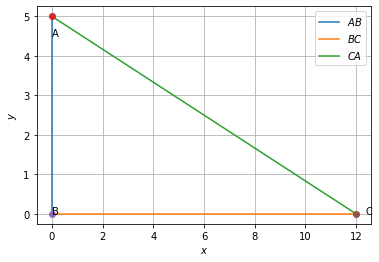
\includegraphics[width= \columnwidth]{solutions/july/2/1/figure1.png}
         \caption{The Constructed triangle}
         \label{constr/july/1Figure}
\end{figure}






%
\item Construct $\triangle ABC$  with $BC = 7.5, AC = 5$ and $\angle C = 60\degree$.
\\
\solution

\begin{align}
\because     \vec{A} = b\myvec{\cos C\\ \sin C}, \vec{B} = \myvec{a\\0}, \vec{C} = \myvec{0\\0},
    \end{align}
    substituting the given values, 
    \begin{align}
        \vec{A} = 5\myvec{\cos60\\ \sin60} = \myvec{2.5\\2.5\sqrt3},  \vec{B} = \myvec{7.5\\0},  \vec{C} = \myvec{0\\0}
        \end{align}
    which are plotted in Fig. \ref{constr/july/2Figure}.       

\begin{figure}[!h]
         \centering
         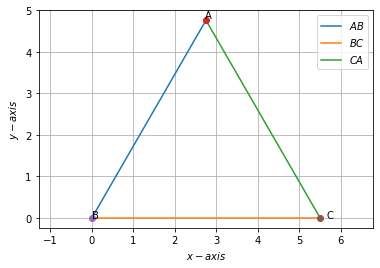
\includegraphics[width= \columnwidth]{solutions/july/2/2/Figures/Figure 1.png}
         \caption{The Constructed triangle}
         \label{constr/july/2Figure}
\end{figure}




\item Construct $\triangle XYZ$ if $XY = 6, \angle X = 30\degree$ and $\angle Y = 100 \degree$.
\item If $AC = 7, \angle A = 60\degree$ and $\angle B = 50 \degree$, can you draw the triangle?
%
\solution
From the given information, 
To find angle C:
\begin{align}
\angle{C} = \ang{70}
\end{align}
and 
\begin{align}
  a&= b\brak{\frac{\sin{A}}{\sin{B}}} 
\\
  &= 7.913611
  \end{align}
%  
Thus, the coordinates are 
\begin{align}
  \vec{C} =\myvec{0 \\ 0},
  \vec{B} =a\myvec{\cos{\ang{70}} \\ \sin{\ang{70}}},
  \vec{A} =\myvec{7 \\ 0}
  \end{align}
  
\begin{figure}[!h]
\centering
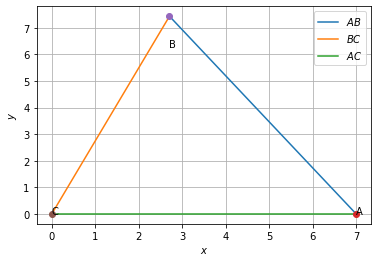
\includegraphics[width=\columnwidth]{solutions/july/2/4/Figure 1.jpeg}
\caption{$\triangle ABC$}
\label{fig:triangle}	
\end{figure}
To find side $a$
The vertices of $\triangle ABC$ are
Lines AB,BC,CA are then generated and plotted using these coordinates to construct $\triangle ABC$
Plot of the $\triangle ABC$:

\end{document}


\item Construct $\triangle PQR$ if $PQ = 5, \angle Q = 105 \degree$ and $\angle R = 40 \degree$.
\item Can you construct $\triangle DEF$ such that $EF = 7.2, \angle E = 110\degree$ and $\angle F = 180\degree$?
\item Construct the  triangles in Table \ref{table:triangle_const_exercises}.
\begin{table}[!ht]
\centering
\input{./chapters/constr/Triangle}
\caption{}
\label{table:triangle_const_exercises}
\end{table}
\solution
\begin{enumerate}
    \item
    \item 
    \solution
    We obtain the vertices of the rhombus as follows
\begin{align}
\vec{A} = \myvec{-3\\0},
\vec{B} = \myvec{0\\-3.5},
\vec{C} = \myvec{3\\0},
\vec{D} = \myvec{0\\3.5}
\end{align}
which are plotted in Fig. \ref{quad/45/fig:Rhombus ABCD}.
%
\begin{figure}[ht!]
\centering
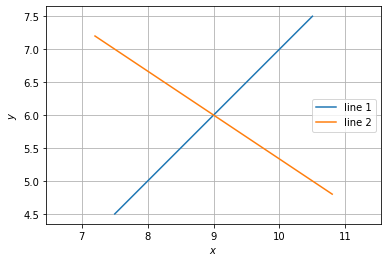
\includegraphics[width=\columnwidth]{solutions/quad/45/figure2.png}
\caption{Rhombus ABCD}
\label{quad/45/fig:Rhombus ABCD}
\end{figure}

    \item 
    \solution
    From the given information,
%
\begin{align}
\angle{C} = \ang{60}
\end{align}
%
Using the sine formula, 
%
\begin{align}
c &= b \brak{\frac{\sin{C}}{\sin{B}}} 
\\
&= 3.3915
\end{align}
%
the vertices of $\triangle ABC$ are
\begin{align}
\vec{A} = \myvec{0 \\ 0},
\vec{B} = c\myvec{\cos{\ang{70}} \\ \sin{\ang{70}}},
\vec{C} = \myvec{3 \\ 0}
\end{align}
and  plotted in Fig. \ref{constr/tri/27/3/fig:triangle ABC}.
%
\begin{figure}[ht]
    \centering
    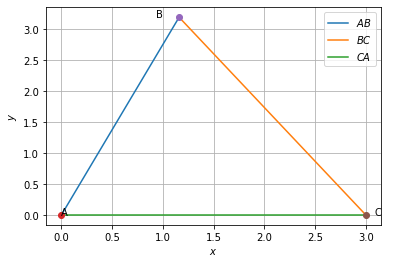
\includegraphics[width=\columnwidth]{solutions/triangle/27/3/Triangle_ABC.PNG}
    \caption{Plot of $\triangle ABC$}
    \label{constr/tri/27/3/fig:triangle ABC}
\end{figure}


        
\end{enumerate}
%

%\subsection{Quadrilateral}
%%\renewcommand{\theequation}{\theenumi}
%\begin{enumerate}[label=\thesubsection.\arabic*.,ref=\thesubsection.\theenumi]
%%\begin{enumerate}[label=\arabic*.,ref=\thesection.\theenumi]
%\numberwithin{equation}{enumi}


\item Construct a quadrilateral $ABCD$ such that $AB=5, \angle A = 50\degree, AC = 4, BD = 5$ and $AD = 6$.
\\
\solution 
\begin{enumerate}
    \item Given point $\vec{P} = \myvec{-4\\3}$ and slope $m = \frac{1}{2}$.
    The direction vector is $\vec{m} = \myvec{2\\1}$.  
    Hence, the normal vector
    \begin{align}
    \label{linform/2/14/eq:line_norm_dir}
    \vec{n} &= \myvec{0&-1\\1&0}\vec{m} 
    \\
    &= \myvec{-1\\2}
    \end{align}
    The equation of the line in terms of the normal vector is then obtained as
    \begin{align}
    \label{linform/2/14/eq:line_norm_vec}
    \vec{n}^T\brak{\vec{x}-\vec{A}} &= 0
    \\
    \implies \myvec{-1 & 2} \vec{x} &= 10
    \end{align}
    See Fig.     \ref{linform/2/14/Plot of Line $AB$ (Part-1)}
    \begin{figure}[ht]
    \centering
    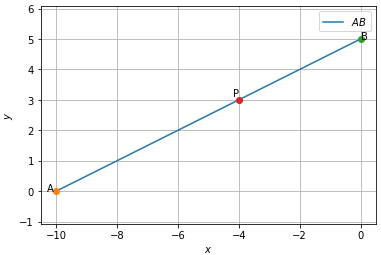
\includegraphics[width=\columnwidth]{solutions/su2021/2/14/Line_Plot_Part1.PNG}
    \caption{Plot of Line $AB$ (Part-1)}
    \label{linform/2/14/Plot of Line $AB$ (Part-1)}
    \end{figure}
    \item Given point $\vec{P} = \myvec{2\\2\sqrt{3}}$.From the given information we have, $\tan75\degree =m = \frac{\sqrt{3}+1}{\sqrt{3}-1}$.
    The direction vector is $\vec{m} = \myvec{1\\\tan75\degree}$.  
    Hence, the normal vector
    \begin{align}
    \label{linform/2/14/eq:line_norm_dir2}
    \vec{n} &= \myvec{0&-1\\1&0}\vec{m} 
    \\
    &= \myvec{-\tan75\degree\\1}
    \end{align}
    The equation of the line in terms of the normal vector is then obtained as
    \begin{align}
    \label{linform/2/14/eq:line_norm_vec2}
    \vec{n}^T\brak{\vec{x}-\vec{A}} &= 0
    \\
    \implies \myvec{-\sqrt{3}+1 &\sqrt{3}-1}  \vec{x} &= -4\brak{\sqrt{3}-1}
    \end{align}
    See Fig. \ref{linform/2/14/Plot of Line $AB$ (Part-2)}

    \begin{figure}[ht]
    \centering
    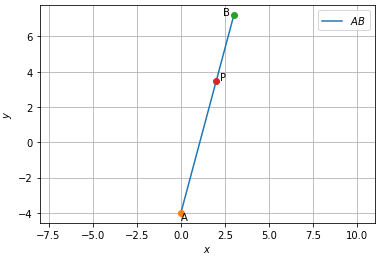
\includegraphics[width=\columnwidth]{solutions/su2021/2/14/Line_Plot_Part2.PNG}
    \caption{Plot of Line $AB$ (Part-2)}
    \label{linform/2/14/Plot of Line $AB$ (Part-2)}
    \end{figure}
\end{enumerate}
\item Construct $PQRS$ where $PQ = 4, QR = 6, RS = 5, PS = 5.5$ and $PR = 7$.
\item Draw $JUMP$ with $JU = 3.5, UM=4, MP = 5, PJ =4.5$ and $PU = 6.5$
\item Construct a quadrilateral $ABCD$ such that $BC=4.5,  AC = 5.5, CD = 5, BD = 7$ and $AD = 5.5$.
\item Can you construct a quadrilateral $PQRS$ with $PQ=3, RS=3, PS=7.5, PR=8$ and $SQ=4$?
\\
\solution 
  
  If we expand the probabilities given further more by substituting the value of x and only considering 0 to 4 hours as the probability of studying in the remaining hours is zero, we get
  
  \begin{table}[ht]
  
 \centering
  
  \begin{tabular}{|c|c|c|c|c|c|}
    \hline
    x &  0 & 1 & 2 & 3 & 4\\
    \hline
    $\Pr\brak{X=x}$ & 0.1& k& 2k & 2k & k\\
    \hline
    
\end{tabular}
\caption{Given probabilities}
\label{Table_1}
\end{table}
we also know that,
\begin{align}
    \sum_{k = 0}^4 \Pr\brak{X = k} = 1 \label{eq 2.0.1}
\end{align}

By substituting the probabilities in \eqref{eq 2.0.1}
\begin{align}
& \implies 0.1 + k + 2k + 2k + k = 1 \\
& \implies 6k = 0.9 \label{eq 2.0.3}
\end{align}

Therefore, from \eqref{eq 2.0.3}
\begin{align}
    k = 0.15
\end{align}
  
 So from \ref{Table_1}
  \begin{table}[ht]
  
  \centering
  \begin{tabular}{|c|c|c|c|c|c|}
    \hline
    x &  0 & 1 & 2 & 3 & 4\\
    \hline
    $\Pr\brak{X=x}$ & 0.1& 0.15& 0.3 & 0.3 & 0.15\\
    \hline
    
\end{tabular} 
\caption{Probabilities after finding k}
\end{table}

\begin{figure}[ht]
    \centering
    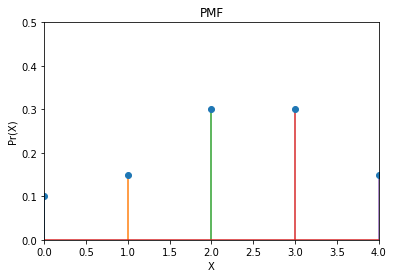
\includegraphics[width=\columnwidth]{solutions/5/28/Figures/PMF.png}
    \caption{Probability Mass Function (PMF)}
    \label{Figure_1}
\end{figure}

We know that, Cumulative Distributive Function (CDF) 
\begin{align}
    F(x) = \Pr\brak{X \le x}
\end{align}

\begin{table}[ht]
  
  \centering
  \begin{tabular}{|c|c|c|c|c|c|}
    \hline
    x &  0 & 1 & 2 & 3 & 4\\
    \hline
    $F(X)$ & 0.1& 0.25& 0.55 & 0.85 & 1\\
    \hline
    
\end{tabular} 
\caption{CDF}
\label{Table_2}
\end{table}

\begin{figure}[ht]
    \centering
    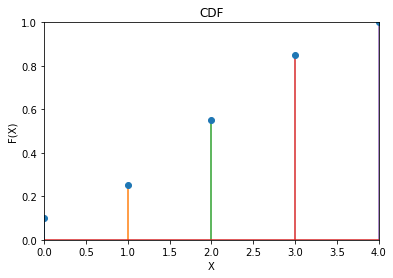
\includegraphics[width=\columnwidth]{solutions/5/28/Figures/CDF.png}
    \caption{Cumulative Distributive Function (CDF)}
    \label{Figure_2}
\end{figure}

And also, 
\begin{align}
     \Pr\brak{x < X \le y} = F\brak{y} - F\brak{x} \label{eq 2.0.6}
\end{align}
         \begin{enumerate}
        \item Probability of studying at least two hours 
           \begin{align}
            & \implies \sum_{k = 2}^4 \Pr\brak{X = k} = \Pr\brak{X \ge 2}\\
            & \implies \Pr\brak{1 < X \le 4} 
        \end{align}
        From \eqref{eq 2.0.6} and \eqref{Table_2}
        \begin{align}
            & = F(4) - F(1)\\
            & = 1 - 0.25\\
            & = 0.75
        \end{align}
        
        \item Probability of studying exactly two hours
        \begin{align}
            & = \Pr\brak{X = 2}\\
            & = 0.3
        \end{align}
        
        \item Probability of studying at most two hours 
        \begin{align}
          & \implies \sum_{k = 0}^2  \Pr\brak{X = k} = \Pr \brak{X \le 2}
         \end{align}
        From \eqref{Table_2}
        \begin{align}
            & = F(2)\\
            & = 0.55
        \end{align}
    \end{enumerate}
  
    \begin{table}[ht]
   
    \centering
  \begin{tabular}{|c|c|c|}
    \hline
    $\Pr\brak{X \geq 2}$ &  $\Pr \brak{X = 2}$ & $\Pr\brak{X \leq 2}$\\
    \hline
     0.75& 0.3& 0.55 \\
    \hline
    Case 1 &Case 2 &Case 3\\
    \hline
\end{tabular} 
 \caption{Final solution}
 \label{Table_3}
\end{table}

\begin{figure}[ht]
    \centering
    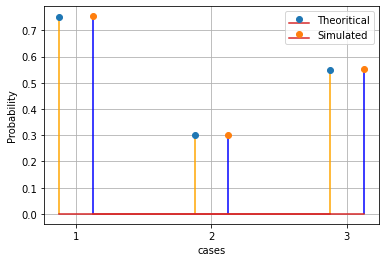
\includegraphics[width=\columnwidth]{solutions/5/28/Figures/stem.png}
    \caption{Simulation and Theoretical Comparison}
    \label{Figure_3}
\end{figure}


\item Construct $LIFT$ such that $LI = 4, IF = 3, TL = 2.5, LF = 4.5, IT=4$.
\item Draw $GOLD$ such that $OL=7.5, GL=6, GD=6, LD = 5, OD = 10$.
\\
\solution 
We obtain the vertices of the rhombus as follows
\begin{align}
\vec{A} = \myvec{-3\\0},
\vec{B} = \myvec{0\\-3.5},
\vec{C} = \myvec{3\\0},
\vec{D} = \myvec{0\\3.5}
\end{align}
which are plotted in Fig. \ref{quad/45/fig:Rhombus ABCD}.
%
\begin{figure}[ht!]
\centering
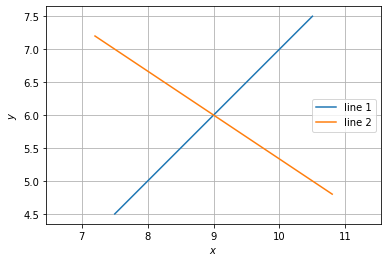
\includegraphics[width=\columnwidth]{solutions/quad/45/figure2.png}
\caption{Rhombus ABCD}
\label{quad/45/fig:Rhombus ABCD}
\end{figure}


\item DRAW rhombus $BEND$ such that $BN = 5.6$, $DE = 6.5$.
\item construct a quadrilateral MIST where $MI = 3.5, IS = 6.5, \angle M = 75 \degree, \angle I = 105 \degree$ and $\angle S = 120 \degree$.
\item Can you construct the above quadrilateral MIST if $\angle M = 100 \degree$ instead of $75 \degree$.
\item Can you constrcut the quadrilateral PLAN if $PL = 6, LA = 9.5, \angle P = 75 \degree, \angle L = 150 \degree$ and $\angle A = 140 \degree$?
\item Construct $MORE$ where $MO = 6, OR = 4.5, \angle M = 60 \degree, \angle O = 105 \degree, \angle R = 105 \degree$.
\item Construct $PLAN$ where $PL = 4, LA = 6.5, \angle P = 90 \degree, \angle A = 110\degree$ and $\angle N = 85\degree$.
\item Draw  rectangle $OKAY$ with $OK = 7$ and $KA = 5$.
\item Construct $ABCD $, where $AB = 4, BC = 5, Cd = 6.5, \angle B = 105 \degree$ and $\angle C = 80\degree$.
\\
\solution 

Let 
    \begin{align}
    &\angle B= 105\degree=\theta \label{quad/42/eq1}
    \\
    &\angle C= 80\degree=\alpha \label{quad/42/eq2}
    \\
    &\norm{\vec{A}-\vec{B}} =4=p \label{quad/42/eq3}
    \\
    &\norm{\vec{C}-\vec{B}} =5=q \label{quad/42/eq4}
    \\
     &\norm{\vec{D}-\vec{C}} =6.5=r \label{quad/42/eq5}
    \end{align}
and 
\begin{align}
    &\vec{B}=\myvec{0\\0}, \vec{C}=\myvec{5\\0}
\end{align}

\begin{lemma}
\label{quad/42/lemma}
\begin{align}
  & \vec{A} = p \vec{b}  \quad \brak{\because \vec{B}=\myvec{0\\0}} \label{quad/42/eq a}
\\
  & \vec{D} =\vec{C} + r \vec{c} \label{quad/42/eq b}
\end{align}
where 
\begin{align}
 \vec{b} = \myvec{\cos B \\ \sin B } ,\vec{c} = \myvec{\cos C\\ \sin C }
\end{align}
\end{lemma}
Thus, 
\begin{align}
 \vec{A} &=4\myvec{\cos 105 \\\sin 105 }
\\
&=\myvec{-1.03\\3.86}
\end{align}
and 
\begin{align}
\vec{D} &=\myvec{5\\0} + 6.5\myvec{\cos 80 \\\sin 80 }
\\
&=\myvec{6.12\\6.39}
\end{align}
which are then used to plot Fig. \ref{quad/42/fig:Quadrilateral ABCD}	
\begin{figure}[!ht]
\centering
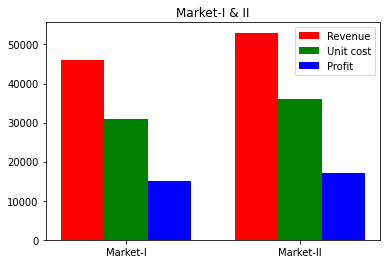
\includegraphics[ width=\columnwidth]{solutions/quad/42/FIGURE.png}
\caption{Quadrilateral ABCD}
\label{quad/42/fig:Quadrilateral ABCD}	
\end{figure}

%
\item Construct $DEAR$ with $DE = 4, EA = 5, AR = 4.5, \angle E = 60 \degree$ and $\angle A = 90 \degree$.
\\
\solution 
We obtain the vertices of the rhombus as follows
\begin{align}
\vec{A} = \myvec{-3\\0},
\vec{B} = \myvec{0\\-3.5},
\vec{C} = \myvec{3\\0},
\vec{D} = \myvec{0\\3.5}
\end{align}
which are plotted in Fig. \ref{quad/45/fig:Rhombus ABCD}.
%
\begin{figure}[ht!]
\centering
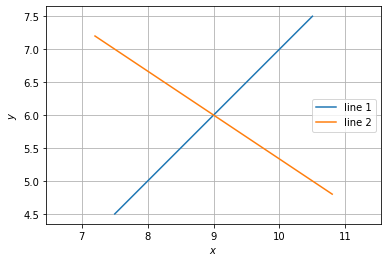
\includegraphics[width=\columnwidth]{solutions/quad/45/figure2.png}
\caption{Rhombus ABCD}
\label{quad/45/fig:Rhombus ABCD}
\end{figure}


\item Construct $TRUE$ with $TR = 3.5, RU = 3, UE = 4 \angle R = 75\degree$ and $\angle U = 120\degree$.
\\
\solution 
We obtain the vertices of the rhombus as follows
\begin{align}
\vec{A} = \myvec{-3\\0},
\vec{B} = \myvec{0\\-3.5},
\vec{C} = \myvec{3\\0},
\vec{D} = \myvec{0\\3.5}
\end{align}
which are plotted in Fig. \ref{quad/45/fig:Rhombus ABCD}.
%
\begin{figure}[ht!]
\centering
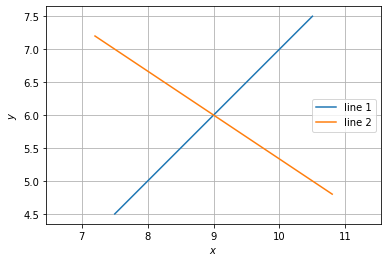
\includegraphics[width=\columnwidth]{solutions/quad/45/figure2.png}
\caption{Rhombus ABCD}
\label{quad/45/fig:Rhombus ABCD}
\end{figure}




\item Can you construct a rhombus $ABCD$ with $AC = 6$ and $BD = 7$?
\\
\solution 
We obtain the vertices of the rhombus as follows
\begin{align}
\vec{A} = \myvec{-3\\0},
\vec{B} = \myvec{0\\-3.5},
\vec{C} = \myvec{3\\0},
\vec{D} = \myvec{0\\3.5}
\end{align}
which are plotted in Fig. \ref{quad/45/fig:Rhombus ABCD}.
%
\begin{figure}[ht!]
\centering
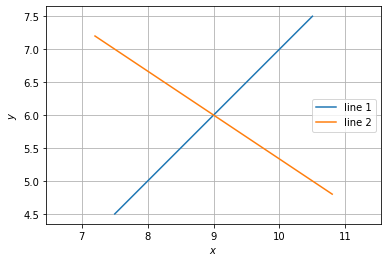
\includegraphics[width=\columnwidth]{solutions/quad/45/figure2.png}
\caption{Rhombus ABCD}
\label{quad/45/fig:Rhombus ABCD}
\end{figure}


\item Draw a square $READ$ with $RE = 5.1$.
\\
\solution 
The centers and radii of the two circles without any loss of generality are given in Table \ref{constr/55/tab:table1}
%
\begin{table}[!ht]
\begin{center}
\begin{tabular}{ | m{2cm} | m{2cm} | m{2cm} |} 
\hline
 & Circle 1 & Circle 2 \\
\hline
Centre  & $\vec{A}$=\myvec{0\\0} & $\vec{B}$=\myvec{3\\0} \\ 
\hline
Radius & $r_{1}=r_{2}=3$  \\ 
\hline
\end{tabular}
\end{center}
\caption{Input values}
\label{constr/55/tab:table1}

\end{table}

% The choice for $\vec{A}$ and $\vec{B}$ is valid as:
% \begin{align}
% \norm{\vec{B}-\vec{A}} = \norm{\vec{A}-\vec{B}}=\norm{\vec{B}}  = 3 \quad \brak{\because \vec{A}=0}
% \end{align}

Let 
\begin{align}
\vec{u}=\myvec{\cos \theta\\  \sin \theta},  \theta \in \sbrak{0,2\pi}.
\end{align}

Then on Circle 1  and Circle 2 are  given by 
\begin{align}
\vec{x}&=\vec{A}+r\vec{u}
\\
\vec{x}&=\vec{B}+r\vec{u}
\end{align}

Fig. \ref{constr/55/fig:circle} is plotted using the above equations.
%
\begin{figure}[!ht]
\centering
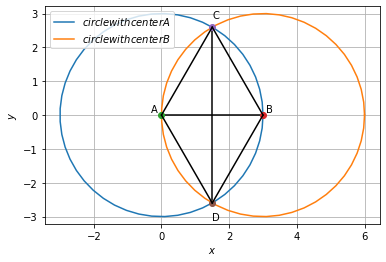
\includegraphics[width=\columnwidth]{solutions/55/Figures/figure3.png}
\caption{Circles with their points of intersection}
\label{constr/55/fig:circle}	
\end{figure}
Fig. \ref{constr/55/fig:circle} 

The general equation of Circle 1 is given by 
\begin{align}
    \norm{\vec{x}-\vec{A}}^2 &= r^2
    \\
\vec{x}^{\top}\vec{x} - 2\vec{A}^{\top}\vec{x} + \norm{\vec{A}}^2 -r_{1}^2 &= 0\label{constr/55/eq:14}
\end{align}
Similarly, for Circle 2,
\begin{align}
\vec{x}^{\top}\vec{x} - 2\vec{B}^{\top}\vec{x} + \norm{\vec{B}}^2 -r_{2}^2 = 0\label{constr/55/eq:15}
\end{align}
Subtracting \eqref{constr/55/eq:15} from \eqref{constr/55/eq:14},
\begin{align}
2\vec{B}^{\top}\vec{x}=\norm{\vec{B}}^2
\\
\myvec{1&0}\vec{x}=\frac{3}{2}
\end{align}
which can be expressed as
\begin{align}
\vec{x} &=\frac{1}{2}\myvec{3\\ 0} + \lambda \myvec{0\\1}\label{constr/55/eq:19}\\
&=\vec{q}+\lambda\vec{m} \text{ where}\label{constr/55/eq:20}\\
\vec{q}&=\myvec{1.5\\ 0},
\vec{m}=\myvec{0\\1}
\end{align}
Substituting \eqref{constr/55/eq:20} in \eqref{constr/55/eq:14}
\begin{align}
\norm{\vec{x}}^2=r^2\quad \brak{\because \vec{A}=0}
\\
\norm{\vec{q}+\lambda\vec{m}}^2=r^2\\
(\vec{q}+\lambda \vec{m})^{\top}(\vec{q}+\lambda \vec{m})=r^2\\
\implies \vec{q}^{\top}(\vec{q}+\lambda \vec{m})+\lambda \vec{m}^{\top}(\vec{q}+\lambda \vec{m})=r^2
\\
\implies \norm{\vec{q}}^2+\lambda\vec{q}^{\top}\vec{m}+\lambda\vec{m}^{\top}\vec{q}+\lambda^2\norm{\vec{m}}^2=r^2
\\
\implies \norm{\vec{q}}^2+2\lambda\vec{q}^{\top}\vec{m}+\lambda^2\norm{\vec{m}}^2=r^2 
% \\
% \implies \lambda(\lambda\norm{\vec{m}}^2+2\vec{q}^{\top}\vec{m})=r^2-\norm{\vec{q}}^2\\
% \implies\lambda^2\norm{\vec{m}}^2=9-\norm{\vec{q}}^2
\\
\implies \lambda=\pm \sqrt{\frac{9-\norm{\vec{q}}^2}{\norm{\vec{m}}^2}} \quad \because \vec{q}^{\top}\vec{m} = 0
% \lambda^2=6.75\\
% \lambda=+\sqrt{6.75},-\sqrt{6.75}
\end{align}
Substituting the value of $\lambda$ in \eqref{constr/55/eq:20},
\begin{align}
%\vec{x}=\vec{q}+\lambda\vec{m}\\
\vec{C}&=\vec{q}+\lambda\vec{m}\\
\vec{D}&=\vec{q}-\lambda\vec{m} \\
\implies (\vec{A}-\vec{B})^{\top}(\vec{C}-\vec{D})
&=2\myvec{-3&0}\myvec{0\\\sqrt{6.75}}
\\
&=0
\\
\implies AB\perp CD
\end{align}


% We have $\vec{C}$ and $\vec{D}$ as points of intersection and $r_{1}=r_{2}$.So,
% \begin{align}
% \norm{\vec{C}-\vec{A}}^2 = \norm{\vec{C}-\vec{B}}^2
% \end{align}
% \begin{align}
% \implies(\vec{C}-\vec{A})^{\top}(\vec{C}-\vec{A})=(\vec{C}-\vec{B})^{\top}(\vec{C}-\vec{B})
% \\
% \implies \vec{A}^{\top}\vec{C}-\vec{B}^{\top}\vec{C}=\vec{C}^{\top}\vec{B}-\vec{C}^{\top}\vec{A}+\norm{\vec{A}}^2-\norm{\vec{B}}^2 
% \end{align}
% \begin{align}
% \implies2\times \vec{A}^{\top}\vec{C}-2\times\vec{B}^{\top}\vec{C}=\norm{\vec{A}}^2-\norm{\vec{B}}^2 \label{constr/55/eq:1}
% \end{align}
% Similarly,using:
% \begin{align}
% \norm{\vec{D}-\vec{A}}^2 = \norm{\vec{D}-\vec{B}}^2
% \end{align}
% We get:
% \begin{align}
% 2\times \vec{A}^{\top}\vec{D}-2\times\vec{B}^{\top}\vec{D}=\norm{\vec{A}}^2-\norm{\vec{B}}^2 \label{constr/55/eq:2}
% \end{align}

% Subtracting equation \ref{constr/55/eq:2} from equation \ref{constr/55/eq:1}:
% \begin{align}
% 2\times(\vec{A}^{\top}-\vec{B}^{\top})(\vec{C}-\vec{D})=0
% \\
% \implies (\vec{A}-\vec{B})^{\top}(\vec{C}-\vec{D})=0
% \\
% \implies AB\perp CD
% \end{align}

\item Draw a rhombus who diagonals are $5.2$ and $6.4$.
\\
\solution 
We obtain the vertices of the rhombus as follows
\begin{align}
\vec{A} = \myvec{-3\\0},
\vec{B} = \myvec{0\\-3.5},
\vec{C} = \myvec{3\\0},
\vec{D} = \myvec{0\\3.5}
\end{align}
which are plotted in Fig. \ref{quad/45/fig:Rhombus ABCD}.
%
\begin{figure}[ht!]
\centering
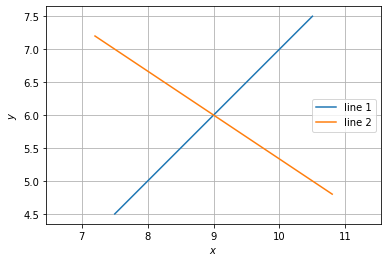
\includegraphics[width=\columnwidth]{solutions/quad/45/figure2.png}
\caption{Rhombus ABCD}
\label{quad/45/fig:Rhombus ABCD}
\end{figure}


\item Draw a rectangle with adjacent sides $5$ and $4$.
\\
\solution 
We obtain the vertices of the rhombus as follows
\begin{align}
\vec{A} = \myvec{-3\\0},
\vec{B} = \myvec{0\\-3.5},
\vec{C} = \myvec{3\\0},
\vec{D} = \myvec{0\\3.5}
\end{align}
which are plotted in Fig. \ref{quad/45/fig:Rhombus ABCD}.
%
\begin{figure}[ht!]
\centering
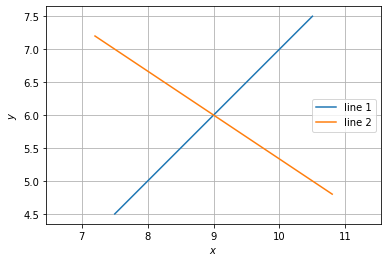
\includegraphics[width=\columnwidth]{solutions/quad/45/figure2.png}
\caption{Rhombus ABCD}
\label{quad/45/fig:Rhombus ABCD}
\end{figure}


\item Draw a parallelogram $OKAY$ with $OK = 5.5$ and $KA = 4.2$.
\\
\solution  There are infinite number of parallelograms that can be draw.  For a unique parallelogram, one angle
needs to be specified.

\item Construct a kite $EASY$ if $AY = 8, EY = 4$ and $SY = 6$.


%\end{enumerate}
%

%\section{Linear Forms}
%\section{Quadratic Forms}
%\subsection{Circle}
%%\renewcommand{\theequation}{\theenumi}
%\begin{enumerate}[label=\thesubsection.\arabic*.,ref=\thesubsection.\theenumi]
%%\begin{enumerate}[label=\arabic*.,ref=\thesection.\theenumi]
%\numberwithin{equation}{enumi}

\item Draw a circle of diameter 6.1

\item With the same centre $\vec{O}$,  draw two circles of radii 4 and 2.5
\\
\solution


All input values required to plot Fig. \ref{constr/52/tab:table1} are given in Table \ref{constr/52/tab:table1} as shown below

\begin{table}[!ht]
\begin{center}
    \resizebox{\columnwidth}{!}{
\begin{tabular}{ | m{2cm} | m{1.5cm}| m{2cm} | m{1.5cm} |} 
\hline
& Symbols & Circle1 & Circle2 \\
\hline
Centre & $\vec{O}$ & \myvec{0\\0} & \myvec{0\\0} \\ 
\hline
Radius & $r_{1}$,$r_{2}$ & 2.5 & 4 \\ 
\hline
Polar coordinate & $\vec{C}_{1}$,$\vec{C}_{2}$ & 2.5\myvec{\cos \theta\\  \sin \theta} & 4\myvec{\cos \theta\\  \sin \theta} \\
\hline
Angle & $\theta$ & 0-2$\pi$ & 0-2$\pi$ \\
\hline
\end{tabular}
    }
\end{center}
\caption{Input values}
\label{constr/52/tab:table1}
\end{table}


\begin{figure}[!ht]
\centering
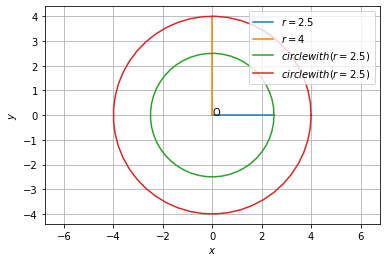
\includegraphics[width=\columnwidth]{solutions/52/Figure3.png}
\caption{Concentric circles with centre as origin and radii 2.5 and 4 respectively}
\label{constr/52/fig:circle}	
\end{figure}


}
\item Draw a circle with centre $\vec{B}$ and radius 6.  If $\vec{C}$ be  a point 10 units  away from its 
centre, construct the pair of tangents $AC$ and $CD$ to the 
circle.
\item Draw a circle of radius 3 and any two of its diameters.  Draw the ends of these diameters. What figure do you get?
\item Let $\vec{A}$ and $\vec{B}$ be the centres of two circles of equal radii 3 such that each one of them passes through the centre of the other.  Let them intersect at $\vec{C}$ and $\vec{D}$.  Is $AB \perp CD$?

\item Construct a tangent to a circle of radius 4 units from a point on the concentric circle of radius 6 
units.
\\
\solution Take the centre of both circles to be at the origin.  
\item Draw a circle of radius 3 units. Take  two points $\vec{P}$ and $\vec{Q}$ on one of its extended 
diameter each at a distance of 7 units from its centre. Draw tangents to the circle from these two points 
$\vec{P}$ and $\vec{Q}$.
\\
\solution Take the diameter to be on the $x$-axis.
\item Draw a pair of tangents to a circle of radius 5 units which are inclined to each other at an angle of 
$60^{\degree}$.
\\
\solution The tangent is perpendicular to the radius.
\item Draw a line segment $AB$ of length 8 units. Taking $\vec{A}$ as centre, draw a circle of radius 4 units 
and taking $\vec{B}$ as centre, draw another circle of radius 3 units. Construct tangents to each circle from 
the centre of the other circle.
\\
\solution Let
\begin{align}
\vec{A} = \myvec{0 \\ 0}, \vec{B} = \myvec{8 \\ 0}.
\end{align}
\item Let ABC be a right triangle in which $a = 8, c = 6$ and $\angle B = 90^{\degree}$.  $BD$ is the 
perpendicular from $\vec{B}$ on $AC$ (altitude). The circle through $\vec{B}, \vec{C}, \vec{D}$ (circumcircle of $\triangle BCD$) is drawn.  Construct the 
tangents from $\vec{A}$ to this circle.
%\\
%\solution Since $\angle BDC = 90\degree$, $BC$ is the diameter of the circumcircle of $\triangle BCD$. Since $AB \perp BC$ and $BC$ is the diameter, $AB$ is a tangent to the circumcircle of $\triangle BCD$.  Let $\vec{O}$ be the centre of the circle.  The point of contact is obtained by rotating $\vec{B}$ by $\theta = 2\angle BAO$. Thus, if 
%\begin{align}
%\vec{B} &= \myvec{0 \\ 0}, \vec{C} = \myvec{a \\ 0},
%\\
%\vec{O} &= \frac{1}{2}\myvec{a \\ 0}
%\end{align}

\item Draw a circle with centre $\vec{C}$ and radius 3.4.  Draw any chord.  Construct the perpendicular bisector of the chord and examine if it passes through $\vec{C}$
%\end{enumerate}
%
%\item Form the differential equation represeting the family of curves given by 
%\begin{align}
%\vec{x}^T \myvec{1 & 0 \\ 0 & 2} \vec{x} -\myvec{2a & 0}\vec{x} = 0,
%\end{align}
%%
%where $a$ is an arbitrary constant.
%%
%\item Form the differntial equation of the family of circles in the first quadrant which touch the coordinate axes.
%\end{enumerate}

%\subsection{Conics}
%\input{./chapters/conics/conics.tex}
%\section{Matrix Decompositions}
%\subsection{QR Decomposition}
%\input{./chapters/decomp/qr.tex}
%\subsection{Singular Value Decomposition}
%\input{./chapters/decomp/svd.tex}
%\section{Inequalities}
%\subsection{Linear Inequalities: Examples}
%%\renewcommand{\theequation}{\theenumi}
%\begin{enumerate}[label=\arabic*.,ref=\thesubsection.\theenumi]
%\numberwithin{equation}{enumi}
    \item Solve $30x < 200$ when
    \begin{enumerate} 
    \item  x is a natural number,
    \item x is an integer.
\end{enumerate}
\solution From the given information, 
\begin{align}
30x < 200 \implies x < \frac{20}{3}
\label{eq:lineq_nat}
\end{align}
If $x$ is a natural number, $x \in \cbrak{1, 2, 3, 4, 5, 6}$. If $x$ is an integer, then the solution set includes 0 as well as all negative integers.
    \item Solve $5x-3 < 3x+1$ when
    \begin{enumerate} 
\item  x is an integer,
    \item x is a real number.
\end{enumerate}
\solution 
\begin{align}
5x-3 < 3x+1 \implies x < 2
\label{eq:lineq_real}
\end{align}
%
If $x$ is real, then $x \in \brak{-\infty, 2}$. 
%Fig.  provides a graphical solution using the following python code
%\begin{lstlisting}
%\end{lstlisting}
    \item Solve the following system of linear inequalities graphically.
\begin{align}
\label{eq:line_two_ineq}
\begin{split}
    x+y &\geq 5
\\
    x-y &\leq 3
\end{split}
\end{align}
\solution  Let $u_1 \ge 0, u_2 \ge 0$.  This may be expressed as
\begin{align}
\vec{u} = \myvec{u_1\\u_2}\succeq \vec{0}
\end{align}
%
\eqref{eq:line_two_ineq} can then be expressed as
\begin{align}
\begin{split}
    x+y &\geq 5
\\
    -x+y &\geq -3
\end{split}
%
\\
\implies 
\myvec{1 & 1 \\ -1 & 1}\vec{x}  &\succeq \myvec{5\\-3}
\\
\myvec{1 & 1 \\ -1 & 1}\vec{x}  -\vec{u}&=\myvec{5\\-3}
\\
\text{or, }
\myvec{1 & 1 \\ -1 & 1}\vec{x} &= \myvec{5\\-3} +\vec{u}
\end{align}
%
resulting in 
\begin{align}
\vec{x} &= \myvec{1 & 1 \\ -1 & 1}^{-1}\myvec{5\\-3} +\myvec{1 & 1 \\ -1 & 1}^{-1}\vec{u}
\\
\text{or, } \vec{x} &= \myvec{4\\1} +\frac{1}{2}\myvec{1 & -1 \\ 1 & 1}\vec{u}
\end{align}
%
after obtaining the  inverse.
%
 Fig. \ref{fig:line_ineq} generated using the following python code shows the region satisfying \eqref{eq:line_two_ineq}

\begin{lstlisting}
codes/line/line_ineq.py
\end{lstlisting}
%
\begin{figure}[!ht]
\includegraphics[width=\columnwidth]{./line/figs/line_ineq.eps}
\caption{}
\label{fig:line_ineq}
\end{figure}
%
\item Solve 
\begin{align}
\begin{split}
2x+y \geq 4
\\ 
x+y \leq 3
\\ 
2x-3y \leq 6
\end{split}
\label{eq:line_mult_ineq}
\end{align}
%
\\
\solution  Fig. \ref{fig:line_ineq_mult} generated using the following python code shows the region satisfying \eqref{eq:line_mult_ineq}

\begin{lstlisting}
codes/line/line_ineq_mult.py
\end{lstlisting}
%
\begin{figure}[!ht]
\includegraphics[width=\columnwidth]{./line/figs/line_ineq_mult.eps}
\caption{}
\label{fig:line_ineq_mult}
\end{figure}
%
\item   Solve    $x+y < 5$ graphically.
\\
\solution 
\input{./solutions/5/chapters/lines/docq6.tex}
%
    \item Solve 
\begin{align}
\myvec{3 & 2 \\ 1 & 4 \\ 1 & 0 \\ 0 & -1 \\ -1 & 0} \vec{x}\preceq \myvec{150\\80\\15\\0\\0}
%3x+2y \leq 150
%\\ 
%x+4y \leq 80
%\\ 
%x \leq 15
%\\ 
%y \geq 0
%\\
%x \geq 0 
\end{align}
%
   
%    \end{enumerate}
\item Solve  x $\geq$ 3, y $\geq$ 2 graphically.
\\
\solution 
%
\begin{align}
    E(X) &= \frac{1}{\sqrt{2\pi}} \int_{-\infty}^{\infty} x e^{-\frac{x^2}{2}}dx\\
    &=0 \quad \brak{ \text{ odd function}}
\end{align}
\begin{align}
    E\brak{X^2}&= \frac{1}{\sqrt{2\pi}}\int_{-\infty}^{\infty} x^2
e^ {-\frac{x^2}{2}} dx \quad \brak{even function}\\
    &= \frac{2}{\sqrt{2\pi}} \int_{0}^{\infty} x^2 e^{-\frac{x^2}{2}} dx\\
    &= \frac{2}{\sqrt{2\pi}}\int_{0}^{\infty}\sqrt{2u}e^{-u} du \quad\brak{Let \frac{x^2}{2}= u}\\
    &= \frac{2}{\sqrt{\pi}} \int_{0}^{\infty} e^{-u} u^{\frac{3}{2}-1} du\\
    &= \frac{2}{\sqrt{\pi}} \Gamma\brak{{\frac{3}{2}}}\\
    &= \frac{1}{\sqrt{\pi}}\Gamma\brak{\frac{1}{2}} \\
    &= 1
\end{align}
where we have used the fact that
\begin{align}
\quad\because \Gamma(n)= (n-1)\Gamma(n-1); \Gamma\brak{\frac{1}{2}}=\sqrt{\pi}
\end{align}
%
Thus, the  variance is
\begin{align}
    \sigma^2 =  E\brak X^2 - E^2\brak X = 1
\end{align}


    \item Solve 7x+3 $<$ 5x+9. Show the graph of the solutions on number line.
\\
\solution 
%
\begin{align}
    E(X) &= \frac{1}{\sqrt{2\pi}} \int_{-\infty}^{\infty} x e^{-\frac{x^2}{2}}dx\\
    &=0 \quad \brak{ \text{ odd function}}
\end{align}
\begin{align}
    E\brak{X^2}&= \frac{1}{\sqrt{2\pi}}\int_{-\infty}^{\infty} x^2
e^ {-\frac{x^2}{2}} dx \quad \brak{even function}\\
    &= \frac{2}{\sqrt{2\pi}} \int_{0}^{\infty} x^2 e^{-\frac{x^2}{2}} dx\\
    &= \frac{2}{\sqrt{2\pi}}\int_{0}^{\infty}\sqrt{2u}e^{-u} du \quad\brak{Let \frac{x^2}{2}= u}\\
    &= \frac{2}{\sqrt{\pi}} \int_{0}^{\infty} e^{-u} u^{\frac{3}{2}-1} du\\
    &= \frac{2}{\sqrt{\pi}} \Gamma\brak{{\frac{3}{2}}}\\
    &= \frac{1}{\sqrt{\pi}}\Gamma\brak{\frac{1}{2}} \\
    &= 1
\end{align}
where we have used the fact that
\begin{align}
\quad\because \Gamma(n)= (n-1)\Gamma(n-1); \Gamma\brak{\frac{1}{2}}=\sqrt{\pi}
\end{align}
%
Thus, the  variance is
\begin{align}
    \sigma^2 =  E\brak X^2 - E^2\brak X = 1
\end{align}

    \item Solve $\frac{3x-4}{2} \geq \frac{x+1}{4}-1$. Show the graph of the solutions on number line.
\\
\solution 
%
\begin{align}
    E(X) &= \frac{1}{\sqrt{2\pi}} \int_{-\infty}^{\infty} x e^{-\frac{x^2}{2}}dx\\
    &=0 \quad \brak{ \text{ odd function}}
\end{align}
\begin{align}
    E\brak{X^2}&= \frac{1}{\sqrt{2\pi}}\int_{-\infty}^{\infty} x^2
e^ {-\frac{x^2}{2}} dx \quad \brak{even function}\\
    &= \frac{2}{\sqrt{2\pi}} \int_{0}^{\infty} x^2 e^{-\frac{x^2}{2}} dx\\
    &= \frac{2}{\sqrt{2\pi}}\int_{0}^{\infty}\sqrt{2u}e^{-u} du \quad\brak{Let \frac{x^2}{2}= u}\\
    &= \frac{2}{\sqrt{\pi}} \int_{0}^{\infty} e^{-u} u^{\frac{3}{2}-1} du\\
    &= \frac{2}{\sqrt{\pi}} \Gamma\brak{{\frac{3}{2}}}\\
    &= \frac{1}{\sqrt{\pi}}\Gamma\brak{\frac{1}{2}} \\
    &= 1
\end{align}
where we have used the fact that
\begin{align}
\quad\because \Gamma(n)= (n-1)\Gamma(n-1); \Gamma\brak{\frac{1}{2}}=\sqrt{\pi}
\end{align}
%
Thus, the  variance is
\begin{align}
    \sigma^2 =  E\brak X^2 - E^2\brak X = 1
\end{align}

    \item The marks obtained by a student of Class XI in first and second terminal examination are 62 and 48, respectively. Find the minimum marks he should get in the annual examination to have an average of at least 60 marks.
\\
\solution 
%
\begin{align}
    E(X) &= \frac{1}{\sqrt{2\pi}} \int_{-\infty}^{\infty} x e^{-\frac{x^2}{2}}dx\\
    &=0 \quad \brak{ \text{ odd function}}
\end{align}
\begin{align}
    E\brak{X^2}&= \frac{1}{\sqrt{2\pi}}\int_{-\infty}^{\infty} x^2
e^ {-\frac{x^2}{2}} dx \quad \brak{even function}\\
    &= \frac{2}{\sqrt{2\pi}} \int_{0}^{\infty} x^2 e^{-\frac{x^2}{2}} dx\\
    &= \frac{2}{\sqrt{2\pi}}\int_{0}^{\infty}\sqrt{2u}e^{-u} du \quad\brak{Let \frac{x^2}{2}= u}\\
    &= \frac{2}{\sqrt{\pi}} \int_{0}^{\infty} e^{-u} u^{\frac{3}{2}-1} du\\
    &= \frac{2}{\sqrt{\pi}} \Gamma\brak{{\frac{3}{2}}}\\
    &= \frac{1}{\sqrt{\pi}}\Gamma\brak{\frac{1}{2}} \\
    &= 1
\end{align}
where we have used the fact that
\begin{align}
\quad\because \Gamma(n)= (n-1)\Gamma(n-1); \Gamma\brak{\frac{1}{2}}=\sqrt{\pi}
\end{align}
%
Thus, the  variance is
\begin{align}
    \sigma^2 =  E\brak X^2 - E^2\brak X = 1
\end{align}

    \item Find all pairs of consecutive odd natural numbers, both of which are larger than 10, such that their sum is less than 40.
\\
\solution 
\input{./solutions/5/chapters/lines/docq15.tex}
    \item Solve 3x+2y $>$ 6 graphically.
\\
\solution 
%
\begin{align}
    E(X) &= \frac{1}{\sqrt{2\pi}} \int_{-\infty}^{\infty} x e^{-\frac{x^2}{2}}dx\\
    &=0 \quad \brak{ \text{ odd function}}
\end{align}
\begin{align}
    E\brak{X^2}&= \frac{1}{\sqrt{2\pi}}\int_{-\infty}^{\infty} x^2
e^ {-\frac{x^2}{2}} dx \quad \brak{even function}\\
    &= \frac{2}{\sqrt{2\pi}} \int_{0}^{\infty} x^2 e^{-\frac{x^2}{2}} dx\\
    &= \frac{2}{\sqrt{2\pi}}\int_{0}^{\infty}\sqrt{2u}e^{-u} du \quad\brak{Let \frac{x^2}{2}= u}\\
    &= \frac{2}{\sqrt{\pi}} \int_{0}^{\infty} e^{-u} u^{\frac{3}{2}-1} du\\
    &= \frac{2}{\sqrt{\pi}} \Gamma\brak{{\frac{3}{2}}}\\
    &= \frac{1}{\sqrt{\pi}}\Gamma\brak{\frac{1}{2}} \\
    &= 1
\end{align}
where we have used the fact that
\begin{align}
\quad\because \Gamma(n)= (n-1)\Gamma(n-1); \Gamma\brak{\frac{1}{2}}=\sqrt{\pi}
\end{align}
%
Thus, the  variance is
\begin{align}
    \sigma^2 =  E\brak X^2 - E^2\brak X = 1
\end{align}

    \item Solve 3x-6 $\geq$ 0 graphically in a two dimensional plane.
\\
\solution 
%
\begin{align}
    E(X) &= \frac{1}{\sqrt{2\pi}} \int_{-\infty}^{\infty} x e^{-\frac{x^2}{2}}dx\\
    &=0 \quad \brak{ \text{ odd function}}
\end{align}
\begin{align}
    E\brak{X^2}&= \frac{1}{\sqrt{2\pi}}\int_{-\infty}^{\infty} x^2
e^ {-\frac{x^2}{2}} dx \quad \brak{even function}\\
    &= \frac{2}{\sqrt{2\pi}} \int_{0}^{\infty} x^2 e^{-\frac{x^2}{2}} dx\\
    &= \frac{2}{\sqrt{2\pi}}\int_{0}^{\infty}\sqrt{2u}e^{-u} du \quad\brak{Let \frac{x^2}{2}= u}\\
    &= \frac{2}{\sqrt{\pi}} \int_{0}^{\infty} e^{-u} u^{\frac{3}{2}-1} du\\
    &= \frac{2}{\sqrt{\pi}} \Gamma\brak{{\frac{3}{2}}}\\
    &= \frac{1}{\sqrt{\pi}}\Gamma\brak{\frac{1}{2}} \\
    &= 1
\end{align}
where we have used the fact that
\begin{align}
\quad\because \Gamma(n)= (n-1)\Gamma(n-1); \Gamma\brak{\frac{1}{2}}=\sqrt{\pi}
\end{align}
%
Thus, the  variance is
\begin{align}
    \sigma^2 =  E\brak X^2 - E^2\brak X = 1
\end{align}
    
\item 2x+y $\geq$ 6, 3x+4y $\leq$ 12.
    \\
    \solution
    
The given system of inequality can be written in matrix form as
\begin{align}
    \myvec{-1 & -2  \\ -1 & 1 \\ 1 & 1\\ 1 & 0 \\ 0 & 1}\vec{x} \succeq \myvec{-10\\0\\1\\0\\0}
\end{align}
which can be further simplified into 
\begin{align}
    \myvec{-1 & -2 \\ 1 & 0 \\ 0&1}\vec{x} \succeq \myvec{-10\\\frac{-1}{2}\\\frac{-1}{2}}
\end{align}
Let the surplus vector be
\begin{align}
    \vec{u} &= \myvec{u_1\\u_2} \succeq 0
\end{align}
\begin{enumerate}
    \item 
    \begin{align}
        \myvec{-1 & -2 \\ 1 & 0}\vec{x} &\succeq \myvec{-10 \\ \frac{-1}{2}}
        \\
        \implies  \myvec{-1 & -2 \\ 1 & 0}\vec{x} &= \myvec{-10 \\ \frac{-1}{2}} + \vec{u}
    \end{align}
    resulting in 
    \begin{align}
        \vec{x} &= \myvec{-1 & -2 \\ 1 & 0}^{-1}\myvec{-10 \\\frac{-1}{2}} + \myvec{-1 & -2 \\ 1 & 0}^{-1}\vec{u}
        \\
        \implies \vec{x} &= \myvec{\frac{1}{2} \\ \frac{19}{4}} + \myvec{0&1\\ \frac{-1}{2}&\frac{-1}{2}}\vec{u}   \label{ineq/58/eq1}
    \end{align}
    \item 
    \begin{align}
        \myvec{-1& -2 \\ 0 & 1}\vec{x} &\succeq \myvec{-10 \\ \frac{-1}{2}}
        \\
        \implies  \myvec{-1& -2 \\ 0 & 1}\vec{x} &= \myvec{-10 \\ \frac{-1}{2}} + \vec{u}
    \end{align}
    resulting in 
    \begin{align}
        \vec{x} &= \myvec{-1& -2 \\ 0 & 1}^{-1}\myvec{-10 \\ \frac{-1}{2}} + \myvec{-1& -2 \\ 0 & 1}^{-1}\vec{u}
        \\
        \implies \vec{x} &= \myvec{9\\\frac{1}{2}} + \myvec{-1& -2 \\ 0 & 1}\vec{u} \label{ineq/58/eq2}
    \end{align}
\end{enumerate}
Now,solution region which is common to regions of eq. \eqref{ineq/58/eq1} and eq. \eqref{ineq/58/eq2},is given by
\begin{align}
    \boxed{\vec{x} = \myvec{\frac{1}{2}\\\frac{1}{2}}+\myvec{0&1\\\frac{-1}{2}&1}\vec{u}}
\end{align}
%
\begin{figure}[!ht]
\centering
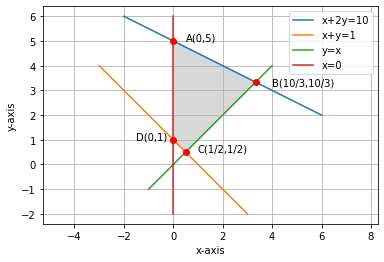
\includegraphics[width=\columnwidth]{solutions/su2021/2/58/Figures/Figure_2.58.png}
\caption{Graphical Solution}
\label{ineq/58/fig:fig1}	
\end{figure}

\begin{figure}[!ht]
\centering
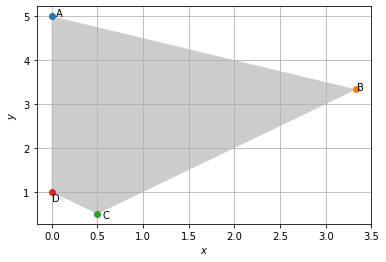
\includegraphics[width=\columnwidth]{solutions/su2021/2/58/Figures/2.58(2).png}
\caption{Magnified Solution region}
\label{ineq/58/fig:fig2}	
\end{figure}


    \item 2x-y $>$ 1, x-2y $<$ -1.
    \\
    \solution
    
%
Let
\begin{align}
\label{eq:1}
\begin{split}
2x-y &> 1,
\\-x+2y &> 1.
\end{split}
\end{align}
\\
Let $u_1 > 0, u_2 > 0$. This may be expressed as
\begin{align}
\vec{u} = \myvec{u_1\\u_2} &> \vec{0}
\end{align}
Now we have,
\begin{align}
\myvec{2&-1 \\ -1&2 }\vec{x} &> \myvec{1 \\ 1}   
\\
\myvec{2&-1 \\ -1&2 }\vec{x}-\vec{u} &= \myvec{1 \\ 1} 
\\
\text{or, } \myvec{2&-1 \\ -1&2 }\vec{x} &= \myvec{1 \\ 1}  + \vec{u}
\end{align}
Resulting in
\begin{align}
\vec{x} &= \myvec{2 & -1 \\ -1 & 2}^{-1}\myvec{1 \\ 1} +\myvec{2 & -1 \\ -1 & 2}^{-1} \vec{u}
\\
\vec{x }&=\myvec{1 \\ 1} +\frac{1}{3}\myvec{2 & 1 \\ 1 & 2}\vec{u}
\end{align} 
Thus , the solution of the system of inequalities can be determined graphically and the desired region is the shaded triangle which is represented in Fig. \ref{fig: Graphical Solution}
\begin{figure}[!ht]
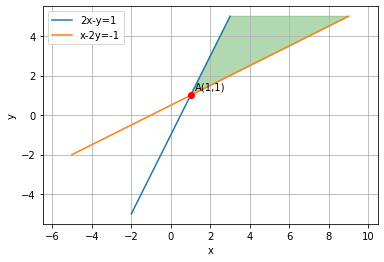
\includegraphics[width=\columnwidth]{solutions/su2021/2/50/Graphical Solution.png}
\caption{Graphical Solution}
\label{fig: Graphical Solution}
\end{figure}



    We obtain the vertices of the rhombus as follows
\begin{align}
\vec{A} = \myvec{-3\\0},
\vec{B} = \myvec{0\\-3.5},
\vec{C} = \myvec{3\\0},
\vec{D} = \myvec{0\\3.5}
\end{align}
which are plotted in Fig. \ref{quad/45/fig:Rhombus ABCD}.
%
\begin{figure}[ht!]
\centering
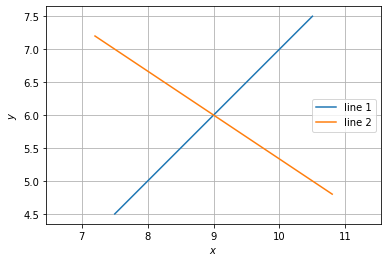
\includegraphics[width=\columnwidth]{solutions/quad/45/figure2.png}
\caption{Rhombus ABCD}
\label{quad/45/fig:Rhombus ABCD}
\end{figure}

    \item 2x+y $\geq$ 8, x+2y $\geq$ 10.
    \\
    \solution
    We obtain the vertices of the rhombus as follows
\begin{align}
\vec{A} = \myvec{-3\\0},
\vec{B} = \myvec{0\\-3.5},
\vec{C} = \myvec{3\\0},
\vec{D} = \myvec{0\\3.5}
\end{align}
which are plotted in Fig. \ref{quad/45/fig:Rhombus ABCD}.
%
\begin{figure}[ht!]
\centering
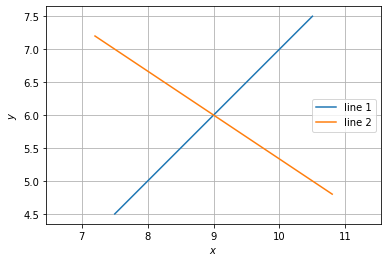
\includegraphics[width=\columnwidth]{solutions/quad/45/figure2.png}
\caption{Rhombus ABCD}
\label{quad/45/fig:Rhombus ABCD}
\end{figure}

    \item 3x+4y $\leq$ 60, x+3y $\leq$ 30, x $\geq$ 0, y $\geq$ 0.
    \\
    \solution
    
From the given inequalities we have,
\begin{align}
    \myvec{-3&-4 \\ -1&-3 \\ 1&0 \\ 0&1}\vec{x} \succeq \myvec{-60 \\ -30 \\ 0 \\ 0}
\end{align}
Which can be further written as
\begin{align}
   \myvec{-3&-4 \\ -1&-3 }\vec{x} \succeq \myvec{-60 \\ -30} 
\end{align}
Let $u_1 \ge 0, u_2 \ge 0$.  This may be expressed as
\begin{align}
\vec{u} = \myvec{u_1\\u_2}\succeq \vec{0}
\end{align}
Now we have,
\begin{align}
  \myvec{-3&-4 \\ -1&-3 }\vec{x} \succeq \myvec{-60 \\ -30}  + \vec{u} 
\end{align}
\begin{align}
        \vec{x} = \myvec{-3 & -4 \\ -1 & -3}^{-1}\myvec{-60 \\ -30} + \myvec{-3 & -4 \\ -1 & -3}^{-1}\vec{u}
        \\
        \implies \vec{x} = \frac{1}{5}\myvec{60 \\ 30}+\frac{1}{5}\myvec{-3&4 \\ 1&-3}\vec{u}
        \\
        \vec{x}=\myvec{12 \\ 6}+\frac{1}{5}\myvec{-3&4 \\ 1&-3}\vec{u}
    \end{align}
Thus the solution of the system of inequalities can be determined graphically, which is represented in Fig.     \ref{ineq/2/55/Graphical solution}.
%
\begin{figure}[ht]
    \centering
    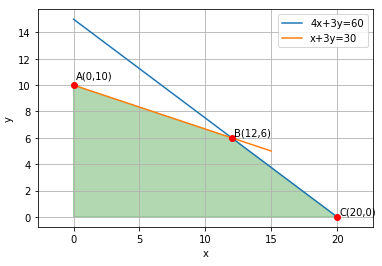
\includegraphics[width=\columnwidth]{solutions/su2021/2/55/Graphical solution region.PNG}
    \caption{Graphical solution}
    \label{ineq/2/55/Graphical solution}
\end{figure}






    \item x-2y $\leq$ 3, 3x+4y $\geq$ 12, x $\geq$ 0, y $\geq$ 1.
    \\
    \solution
    


\begin{figure}[!ht]
    \centering
    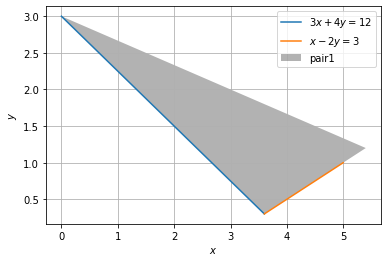
\includegraphics[width=\columnwidth]{solutions/su2021/2/56/Figure9_1.png}
    \caption{Inequality pair 1}
    \label{ineq/56/fig:inequalities1}	
    \end{figure}
    
    \begin{figure}[!ht]
    \centering
    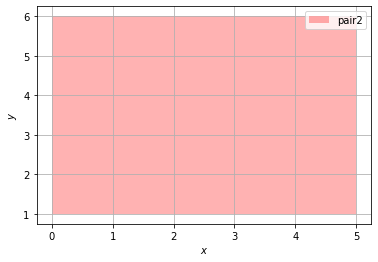
\includegraphics[width=\columnwidth]{solutions/su2021/2/56/Figure9_2.png}
    \caption{Inequality pair 2}
    \label{ineq/56/fig:inequalities2}	
    \end{figure}
    
    \begin{figure}[!ht]
    \centering
    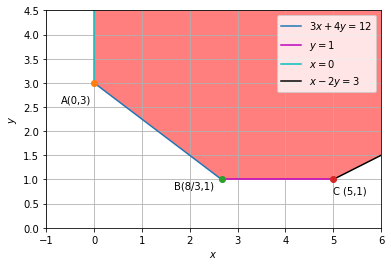
\includegraphics[width=\columnwidth]{solutions/su2021/2/56/Figure 9_3.png}
    \caption{Intersection of \ref{ineq/56/fig:inequalities1} and \ref{ineq/56/fig:inequalities2}}
    \label{ineq/56/fig:inequality3}	
    \end{figure}
    The common region shown by \ref{ineq/56/fig:inequality3} is the solution of set of inequalities.
    
    \item 4x+3y $\leq$ 60, y $\geq$ 2x, x $\geq$ 3, x,y $\geq$ 0.
    \\
    \solution
    

The given system of inequality can be written in matrix form as
\begin{align}
    \myvec{-4 & -3 \\ -2 & 1 \\ 1 & 0 \\ 1 & 0 \\ 0 & 1}\vec{x} \succeq \myvec{-60\\0\\3\\0\\0}
\end{align}
which can be further simplified into 
\begin{align}
    \myvec{-4 & -3 \\ 1 & 0 \\ 0 & 1}\vec{x} \succeq \myvec{-60\\3\\6}
\end{align}

Let the surplus vector be
\begin{align}
    \vec{u} &= \myvec{u_1\\u_2} \succeq 0
\end{align}

\begin{enumerate}
    \item 
    \begin{align}
        \myvec{-4 & -3 \\ 1 & 0}\vec{x} &\succeq \myvec{-60 \\ 3}
        \\
        \implies  \myvec{-4 & -3 \\ 1 & 0}\vec{x} &= \myvec{-60 \\ 3} + \vec{u}
    \end{align}
    resulting in 
    \begin{align}
        \vec{x} &= \myvec{-4 & -3 \\1 & 0}^{-1}\myvec{-60 \\ 3} + \myvec{-4 & -3 \\1 & 0}^{-1}\vec{u}
        \\
        \implies \vec{x} &= \myvec{3 \\16} + \myvec{0 & 1\\ \frac{-1}{3} & \frac{-4}{3}}\vec{u}   \label{ineq/2/57eq1}
    \end{align}

    \item 
    \begin{align}
        \myvec{-4 & -3 \\ 0 & 1}\vec{x} &\succeq \myvec{-60 \\ 6}
        \\
        \implies  \myvec{-4 & -3 \\ 0 & 1}\vec{x} &= \myvec{-60 \\ 6} + \vec{u}
    \end{align}
    resulting in 
    \begin{align}
        \vec{x} &= \myvec{-4 & -3 \\0 & 1}^{-1}\myvec{-60 \\ 6} + \myvec{-4 & -3 \\0 & 1}^{-1}\vec{u}
        \\
        \implies \vec{x} &= \myvec{\frac{21}{2} \\6} + \myvec{\frac{-1}{4} & \frac{-3}{4}\\ 0 & 1}\vec{u} \label{ineq/2/57eq2}
    \end{align}
\end{enumerate}

Now,solution region which is common to regions of eq. \eqref{ineq/2/57eq1} and eq. \eqref{ineq/2/57eq2},is given by

\begin{align}
    \boxed{\vec{x} = \myvec{3 \\ 6}+\myvec{0 & 1\\\frac{1}{12} & \frac{-13}{12}}\vec{u}}
\end{align}


\begin{figure}[!ht]
\centering
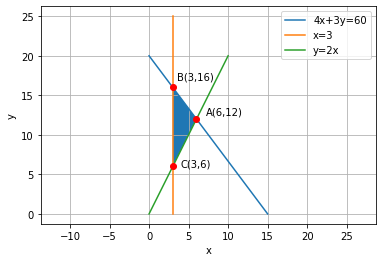
\includegraphics[width=\columnwidth]{solutions/su2021/2/57/Figures/Figure11_1.png}
\caption{Solution Region}
\label{ineq/2/57fig:fig1}	
\end{figure}

% \numberwithin{figure}{section}
% \begin{figure}[!ht]
% \centering
% 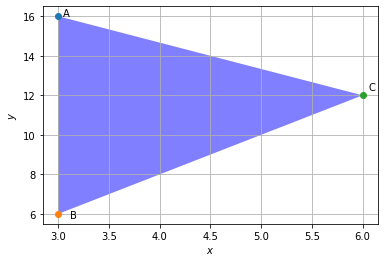
\includegraphics[width=\columnwidth]{Figure11_2}
% \caption{Magnified Solution Region}
% \label{ineq/2/57fig:fig2}	
% \end{figure}




%\end{document}


%
%\subsection{Linear Inequalities: Exercises}
%%\renewcommand{\theequation}{\theenumi}
%\begin{enumerate}[label=\arabic*.,ref=\thesubsection.\theenumi]
%\numberwithin{equation}{enumi}

\item Solve  x $\geq$ 3, y $\geq$ 2 graphically.
\\
\solution 
%
\begin{align}
    E(X) &= \frac{1}{\sqrt{2\pi}} \int_{-\infty}^{\infty} x e^{-\frac{x^2}{2}}dx\\
    &=0 \quad \brak{ \text{ odd function}}
\end{align}
\begin{align}
    E\brak{X^2}&= \frac{1}{\sqrt{2\pi}}\int_{-\infty}^{\infty} x^2
e^ {-\frac{x^2}{2}} dx \quad \brak{even function}\\
    &= \frac{2}{\sqrt{2\pi}} \int_{0}^{\infty} x^2 e^{-\frac{x^2}{2}} dx\\
    &= \frac{2}{\sqrt{2\pi}}\int_{0}^{\infty}\sqrt{2u}e^{-u} du \quad\brak{Let \frac{x^2}{2}= u}\\
    &= \frac{2}{\sqrt{\pi}} \int_{0}^{\infty} e^{-u} u^{\frac{3}{2}-1} du\\
    &= \frac{2}{\sqrt{\pi}} \Gamma\brak{{\frac{3}{2}}}\\
    &= \frac{1}{\sqrt{\pi}}\Gamma\brak{\frac{1}{2}} \\
    &= 1
\end{align}
where we have used the fact that
\begin{align}
\quad\because \Gamma(n)= (n-1)\Gamma(n-1); \Gamma\brak{\frac{1}{2}}=\sqrt{\pi}
\end{align}
%
Thus, the  variance is
\begin{align}
    \sigma^2 =  E\brak X^2 - E^2\brak X = 1
\end{align}


    \item Solve 7x+3 $<$ 5x+9. Show the graph of the solutions on number line.
\\
\solution 
%
\begin{align}
    E(X) &= \frac{1}{\sqrt{2\pi}} \int_{-\infty}^{\infty} x e^{-\frac{x^2}{2}}dx\\
    &=0 \quad \brak{ \text{ odd function}}
\end{align}
\begin{align}
    E\brak{X^2}&= \frac{1}{\sqrt{2\pi}}\int_{-\infty}^{\infty} x^2
e^ {-\frac{x^2}{2}} dx \quad \brak{even function}\\
    &= \frac{2}{\sqrt{2\pi}} \int_{0}^{\infty} x^2 e^{-\frac{x^2}{2}} dx\\
    &= \frac{2}{\sqrt{2\pi}}\int_{0}^{\infty}\sqrt{2u}e^{-u} du \quad\brak{Let \frac{x^2}{2}= u}\\
    &= \frac{2}{\sqrt{\pi}} \int_{0}^{\infty} e^{-u} u^{\frac{3}{2}-1} du\\
    &= \frac{2}{\sqrt{\pi}} \Gamma\brak{{\frac{3}{2}}}\\
    &= \frac{1}{\sqrt{\pi}}\Gamma\brak{\frac{1}{2}} \\
    &= 1
\end{align}
where we have used the fact that
\begin{align}
\quad\because \Gamma(n)= (n-1)\Gamma(n-1); \Gamma\brak{\frac{1}{2}}=\sqrt{\pi}
\end{align}
%
Thus, the  variance is
\begin{align}
    \sigma^2 =  E\brak X^2 - E^2\brak X = 1
\end{align}

    \item Solve $\frac{3x-4}{2} \geq \frac{x+1}{4}-1$. Show the graph of the solutions on number line.
\\
\solution 
%
\begin{align}
    E(X) &= \frac{1}{\sqrt{2\pi}} \int_{-\infty}^{\infty} x e^{-\frac{x^2}{2}}dx\\
    &=0 \quad \brak{ \text{ odd function}}
\end{align}
\begin{align}
    E\brak{X^2}&= \frac{1}{\sqrt{2\pi}}\int_{-\infty}^{\infty} x^2
e^ {-\frac{x^2}{2}} dx \quad \brak{even function}\\
    &= \frac{2}{\sqrt{2\pi}} \int_{0}^{\infty} x^2 e^{-\frac{x^2}{2}} dx\\
    &= \frac{2}{\sqrt{2\pi}}\int_{0}^{\infty}\sqrt{2u}e^{-u} du \quad\brak{Let \frac{x^2}{2}= u}\\
    &= \frac{2}{\sqrt{\pi}} \int_{0}^{\infty} e^{-u} u^{\frac{3}{2}-1} du\\
    &= \frac{2}{\sqrt{\pi}} \Gamma\brak{{\frac{3}{2}}}\\
    &= \frac{1}{\sqrt{\pi}}\Gamma\brak{\frac{1}{2}} \\
    &= 1
\end{align}
where we have used the fact that
\begin{align}
\quad\because \Gamma(n)= (n-1)\Gamma(n-1); \Gamma\brak{\frac{1}{2}}=\sqrt{\pi}
\end{align}
%
Thus, the  variance is
\begin{align}
    \sigma^2 =  E\brak X^2 - E^2\brak X = 1
\end{align}

    \item The marks obtained by a student of Class XI in first and second terminal examination are 62 and 48, respectively. Find the minimum marks he should get in the annual examination to have an average of at least 60 marks.
\\
\solution 
%
\begin{align}
    E(X) &= \frac{1}{\sqrt{2\pi}} \int_{-\infty}^{\infty} x e^{-\frac{x^2}{2}}dx\\
    &=0 \quad \brak{ \text{ odd function}}
\end{align}
\begin{align}
    E\brak{X^2}&= \frac{1}{\sqrt{2\pi}}\int_{-\infty}^{\infty} x^2
e^ {-\frac{x^2}{2}} dx \quad \brak{even function}\\
    &= \frac{2}{\sqrt{2\pi}} \int_{0}^{\infty} x^2 e^{-\frac{x^2}{2}} dx\\
    &= \frac{2}{\sqrt{2\pi}}\int_{0}^{\infty}\sqrt{2u}e^{-u} du \quad\brak{Let \frac{x^2}{2}= u}\\
    &= \frac{2}{\sqrt{\pi}} \int_{0}^{\infty} e^{-u} u^{\frac{3}{2}-1} du\\
    &= \frac{2}{\sqrt{\pi}} \Gamma\brak{{\frac{3}{2}}}\\
    &= \frac{1}{\sqrt{\pi}}\Gamma\brak{\frac{1}{2}} \\
    &= 1
\end{align}
where we have used the fact that
\begin{align}
\quad\because \Gamma(n)= (n-1)\Gamma(n-1); \Gamma\brak{\frac{1}{2}}=\sqrt{\pi}
\end{align}
%
Thus, the  variance is
\begin{align}
    \sigma^2 =  E\brak X^2 - E^2\brak X = 1
\end{align}

    \item Find all pairs of consecutive odd natural numbers, both of which are larger than 10, such that their sum is less than 40.
\\
\solution 
\input{./solutions/5/chapters/lines/docq15.tex}
    \item Solve 3x+2y $>$ 6 graphically.
\\
\solution 
%
\begin{align}
    E(X) &= \frac{1}{\sqrt{2\pi}} \int_{-\infty}^{\infty} x e^{-\frac{x^2}{2}}dx\\
    &=0 \quad \brak{ \text{ odd function}}
\end{align}
\begin{align}
    E\brak{X^2}&= \frac{1}{\sqrt{2\pi}}\int_{-\infty}^{\infty} x^2
e^ {-\frac{x^2}{2}} dx \quad \brak{even function}\\
    &= \frac{2}{\sqrt{2\pi}} \int_{0}^{\infty} x^2 e^{-\frac{x^2}{2}} dx\\
    &= \frac{2}{\sqrt{2\pi}}\int_{0}^{\infty}\sqrt{2u}e^{-u} du \quad\brak{Let \frac{x^2}{2}= u}\\
    &= \frac{2}{\sqrt{\pi}} \int_{0}^{\infty} e^{-u} u^{\frac{3}{2}-1} du\\
    &= \frac{2}{\sqrt{\pi}} \Gamma\brak{{\frac{3}{2}}}\\
    &= \frac{1}{\sqrt{\pi}}\Gamma\brak{\frac{1}{2}} \\
    &= 1
\end{align}
where we have used the fact that
\begin{align}
\quad\because \Gamma(n)= (n-1)\Gamma(n-1); \Gamma\brak{\frac{1}{2}}=\sqrt{\pi}
\end{align}
%
Thus, the  variance is
\begin{align}
    \sigma^2 =  E\brak X^2 - E^2\brak X = 1
\end{align}

    \item Solve 3x-6 $\geq$ 0 graphically in a two dimensional plane.
\\
\solution 
%
\begin{align}
    E(X) &= \frac{1}{\sqrt{2\pi}} \int_{-\infty}^{\infty} x e^{-\frac{x^2}{2}}dx\\
    &=0 \quad \brak{ \text{ odd function}}
\end{align}
\begin{align}
    E\brak{X^2}&= \frac{1}{\sqrt{2\pi}}\int_{-\infty}^{\infty} x^2
e^ {-\frac{x^2}{2}} dx \quad \brak{even function}\\
    &= \frac{2}{\sqrt{2\pi}} \int_{0}^{\infty} x^2 e^{-\frac{x^2}{2}} dx\\
    &= \frac{2}{\sqrt{2\pi}}\int_{0}^{\infty}\sqrt{2u}e^{-u} du \quad\brak{Let \frac{x^2}{2}= u}\\
    &= \frac{2}{\sqrt{\pi}} \int_{0}^{\infty} e^{-u} u^{\frac{3}{2}-1} du\\
    &= \frac{2}{\sqrt{\pi}} \Gamma\brak{{\frac{3}{2}}}\\
    &= \frac{1}{\sqrt{\pi}}\Gamma\brak{\frac{1}{2}} \\
    &= 1
\end{align}
where we have used the fact that
\begin{align}
\quad\because \Gamma(n)= (n-1)\Gamma(n-1); \Gamma\brak{\frac{1}{2}}=\sqrt{\pi}
\end{align}
%
Thus, the  variance is
\begin{align}
    \sigma^2 =  E\brak X^2 - E^2\brak X = 1
\end{align}
    
\item Solve y $<$ 2 graphically.
    \item Solve the following system of inequalities graphically.
     5x+4y $\leq$ 40
     x $\geq$ 2
     y $\geq$ 3
     \item Solve the following system of inequalities graphically.
     8x+3y $\leq$ 100
     x $\geq$ 0
     y $\geq$ 0
     \item Solve the following system of inequalities graphically.
     x+2y $\leq$ 8
     2x+y $\leq$ 8
     x $\geq$ 0
     y $\geq$ 0
     \item Solve -8 $\leq$ 5x-3 $<$ 7.
     \item Solve -5 $\leq \frac{5-3x}{2} \leq 8$.
     \item Solve the system inequalities:
     3x-7 $<$ 5+x
     11-5x $\leq$ 1
     and represent the solutions on the number line.
    
    \item Solve 4x+3 $<$ 6x+7.
    \item Solve $\frac{5-2x}{3} \leq \frac{x}{6}-5$.

	\item Solve 24x $<$ 100, when
	(i) x is a natural number.
	(ii) x is an integer.
	\item Solve -12x $>$ 30, when
	(i) x is a natural number.
	(ii) x is an integer.
	\item Solve 5x-3 $<$ 7, when
	(i) x is an integer.
	(ii) x is a real number.
	\item Solve 3x+8 $>$ 2, when
	(i) x is an integer.
	(ii) x is a real number
	
	\item 4x+3 $<$ 5x+7.
	\item 3x-7 $>$ 5x-1.
	\item 3(x-1) $\geq$ 2(x-3).
	\item 3(2-x) $\leq$ 2(1-x).
	\item x+$\frac{x}{2}+\frac{x}{3}$ $<$ 11.
	\item $\frac{x}{3}\>\frac{x}{2}$+1.
	\item $\frac{3(x-2)}{5}\leq\frac{5(2-x)}{3}$.
	\item $ \frac{1}{2}$($\frac{3x}{5}$+4)$\geq\frac{1}{3}(x-6)$.
	\item 2(2x+3)-10 $<$ 6(x-2).
	\item 37-(3x+5) $\geq$ 9x-8(x-3).
	\item $\frac{x}{4}<\frac{(5x-2)}{3}-\frac{(7x-3)}{5}$.
	\item $\frac{(2x-1)}{3}\geq\frac{(3x-2)}{4}-\frac{(2-x)}{5}$.
	
    \item 3x-2 $<$ 2x+1.
    \item 5x-3 $\geq$ 3x-5.
    \item 3(1-x) $<$ 2(x+4).
    \item $\frac{x}{2}\geq\frac{(5x-2)}{3}-\frac{(7x-3)}{5}$.

    \item x+y $<$ 5.
    \item 2x+y $\geq$ 6.    
    \item 3x+4y $\leq$ 12.
    \item y+8 $\geq$ 2x.
    \item x-y $\leq$ 2.
    \item 2x-3y $>$ 6.
    \item -3x+2y $\geq$ -6.
    \item 3y-5x $<$ 30.
    \item y $<$ -2.
    \item x $>$ -3.
    
    \item 3x+2y $\leq$ 12, x $\geq$ 1, y $\geq$ 2.
    \item 2x+y $\geq$ 6, 3x+4y $\leq$ 12.
    \item x+y $\geq$ 4, 2x-y $<$ 0.
    \item 2x-y $>$ 1, x-2y $<$ -1.
    \item x+y $\leq$ 6, x+y $\geq$ 4.
    \item 2x+y $\geq$ 8, x+2y $\geq$ 10.
    \item x+y $\leq$ 9, y $>$ x, x $\geq$ 0.
    \item 5x+4y $\leq$ 20, x $\geq$ 1, y $\geq$ 2.
    \item 3x+4y $\leq$ 60, x+3y $\leq$ 30, x $\geq$ 0, y $\geq$ 0.
    \\
    \solution
    
From the given inequalities we have,
\begin{align}
    \myvec{-3&-4 \\ -1&-3 \\ 1&0 \\ 0&1}\vec{x} \succeq \myvec{-60 \\ -30 \\ 0 \\ 0}
\end{align}
Which can be further written as
\begin{align}
   \myvec{-3&-4 \\ -1&-3 }\vec{x} \succeq \myvec{-60 \\ -30} 
\end{align}
Let $u_1 \ge 0, u_2 \ge 0$.  This may be expressed as
\begin{align}
\vec{u} = \myvec{u_1\\u_2}\succeq \vec{0}
\end{align}
Now we have,
\begin{align}
  \myvec{-3&-4 \\ -1&-3 }\vec{x} \succeq \myvec{-60 \\ -30}  + \vec{u} 
\end{align}
\begin{align}
        \vec{x} = \myvec{-3 & -4 \\ -1 & -3}^{-1}\myvec{-60 \\ -30} + \myvec{-3 & -4 \\ -1 & -3}^{-1}\vec{u}
        \\
        \implies \vec{x} = \frac{1}{5}\myvec{60 \\ 30}+\frac{1}{5}\myvec{-3&4 \\ 1&-3}\vec{u}
        \\
        \vec{x}=\myvec{12 \\ 6}+\frac{1}{5}\myvec{-3&4 \\ 1&-3}\vec{u}
    \end{align}
Thus the solution of the system of inequalities can be determined graphically, which is represented in Fig.     \ref{ineq/2/55/Graphical solution}.
%
\begin{figure}[ht]
    \centering
    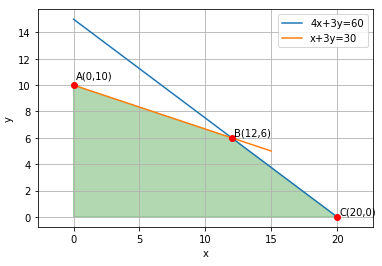
\includegraphics[width=\columnwidth]{solutions/su2021/2/55/Graphical solution region.PNG}
    \caption{Graphical solution}
    \label{ineq/2/55/Graphical solution}
\end{figure}






    
    \item x-2y $\leq$ 3, 3x+4y $\geq$ 12, x $\geq$ 0, y $\geq$ 1.
    \item 4x+3y $\leq$ 60, y $\geq$ 2x, x $\geq$ 3, x,y $\geq$ 0.
    \\
    \solution
    

The given system of inequality can be written in matrix form as
\begin{align}
    \myvec{-4 & -3 \\ -2 & 1 \\ 1 & 0 \\ 1 & 0 \\ 0 & 1}\vec{x} \succeq \myvec{-60\\0\\3\\0\\0}
\end{align}
which can be further simplified into 
\begin{align}
    \myvec{-4 & -3 \\ 1 & 0 \\ 0 & 1}\vec{x} \succeq \myvec{-60\\3\\6}
\end{align}

Let the surplus vector be
\begin{align}
    \vec{u} &= \myvec{u_1\\u_2} \succeq 0
\end{align}

\begin{enumerate}
    \item 
    \begin{align}
        \myvec{-4 & -3 \\ 1 & 0}\vec{x} &\succeq \myvec{-60 \\ 3}
        \\
        \implies  \myvec{-4 & -3 \\ 1 & 0}\vec{x} &= \myvec{-60 \\ 3} + \vec{u}
    \end{align}
    resulting in 
    \begin{align}
        \vec{x} &= \myvec{-4 & -3 \\1 & 0}^{-1}\myvec{-60 \\ 3} + \myvec{-4 & -3 \\1 & 0}^{-1}\vec{u}
        \\
        \implies \vec{x} &= \myvec{3 \\16} + \myvec{0 & 1\\ \frac{-1}{3} & \frac{-4}{3}}\vec{u}   \label{ineq/2/57eq1}
    \end{align}

    \item 
    \begin{align}
        \myvec{-4 & -3 \\ 0 & 1}\vec{x} &\succeq \myvec{-60 \\ 6}
        \\
        \implies  \myvec{-4 & -3 \\ 0 & 1}\vec{x} &= \myvec{-60 \\ 6} + \vec{u}
    \end{align}
    resulting in 
    \begin{align}
        \vec{x} &= \myvec{-4 & -3 \\0 & 1}^{-1}\myvec{-60 \\ 6} + \myvec{-4 & -3 \\0 & 1}^{-1}\vec{u}
        \\
        \implies \vec{x} &= \myvec{\frac{21}{2} \\6} + \myvec{\frac{-1}{4} & \frac{-3}{4}\\ 0 & 1}\vec{u} \label{ineq/2/57eq2}
    \end{align}
\end{enumerate}

Now,solution region which is common to regions of eq. \eqref{ineq/2/57eq1} and eq. \eqref{ineq/2/57eq2},is given by

\begin{align}
    \boxed{\vec{x} = \myvec{3 \\ 6}+\myvec{0 & 1\\\frac{1}{12} & \frac{-13}{12}}\vec{u}}
\end{align}


\begin{figure}[!ht]
\centering
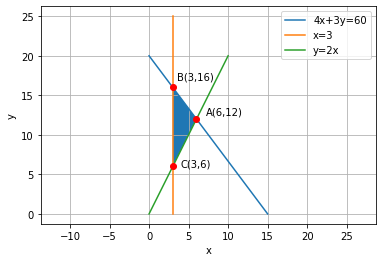
\includegraphics[width=\columnwidth]{solutions/su2021/2/57/Figures/Figure11_1.png}
\caption{Solution Region}
\label{ineq/2/57fig:fig1}	
\end{figure}

% \numberwithin{figure}{section}
% \begin{figure}[!ht]
% \centering
% 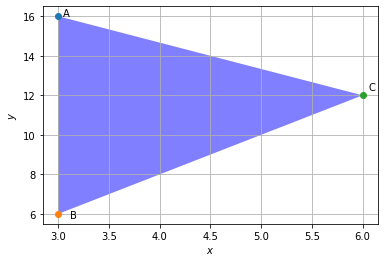
\includegraphics[width=\columnwidth]{Figure11_2}
% \caption{Magnified Solution Region}
% \label{ineq/2/57fig:fig2}	
% \end{figure}




%\end{document}

    \item x+2y $\leq$ 10, x+y $\geq$ 1,x-y $\leq$ 0, x $\geq$ 0, 
    y $\geq$ 0.
    
 
    \item 2 $\leq$ 3x-4 $\leq$ 5.
    \item 6 $\leq$ -3(2x-40)  $<$ 12.
    \item -3 $\leq$ 4-$\frac{7x}{2} \leq 18$. 
    \item -15 $<$ $\frac{3(x-2)}{5} \leq 0$.
    \item -12 $<$ 4-$\frac{3x}{-5} \leq$ 2.
    \item 7 $\leq$ $\frac{(3x+11)}{2} \leq 11$.
    
    \item 5x+1 $>$ -24, 5x-1 $<$ 24.
    \item 2(x-1) $<$ x+5, 3(x+2) $>$ 2-x.
    \item 3x-7 $>$ 2(x-6), 6-x $>$ 11-2x.
    \item 5(2x-7)-3(2x+3) $\leq$ 0, 2x+19 $\leq$ 6x+47.
% \end{enumerate}
    

%\section{Optimization}
\section{Linear Programming}
\renewcommand{\theequation}{\theenumi}
\begin{enumerate}[label=\thesection.\arabic*.,ref=\thesection.\theenumi]
%\begin{enumerate}[label=\arabic*.,ref=\thesubsection.\theenumi]
\numberwithin{equation}{enumi}
%\renewcommand{\theequation}{\theenumi}
%\begin{enumerate}[label=\thesubsection.\arabic*.,ref=\thesubsection.\theenumi]
%%\begin{enumerate}[label=\arabic*.,ref=\thesection.\theenumi]
%\numberwithin{equation}{enumi}

\item Find the maximum and minimum values, if any, of the following functions given by 
%
\begin{enumerate}
\item $f(x) = \brak{2x-1}^2+3$
\\
\solution
%
\begin{align}
    E(X) &= \frac{1}{\sqrt{2\pi}} \int_{-\infty}^{\infty} x e^{-\frac{x^2}{2}}dx\\
    &=0 \quad \brak{ \text{ odd function}}
\end{align}
\begin{align}
    E\brak{X^2}&= \frac{1}{\sqrt{2\pi}}\int_{-\infty}^{\infty} x^2
e^ {-\frac{x^2}{2}} dx \quad \brak{even function}\\
    &= \frac{2}{\sqrt{2\pi}} \int_{0}^{\infty} x^2 e^{-\frac{x^2}{2}} dx\\
    &= \frac{2}{\sqrt{2\pi}}\int_{0}^{\infty}\sqrt{2u}e^{-u} du \quad\brak{Let \frac{x^2}{2}= u}\\
    &= \frac{2}{\sqrt{\pi}} \int_{0}^{\infty} e^{-u} u^{\frac{3}{2}-1} du\\
    &= \frac{2}{\sqrt{\pi}} \Gamma\brak{{\frac{3}{2}}}\\
    &= \frac{1}{\sqrt{\pi}}\Gamma\brak{\frac{1}{2}} \\
    &= 1
\end{align}
where we have used the fact that
\begin{align}
\quad\because \Gamma(n)= (n-1)\Gamma(n-1); \Gamma\brak{\frac{1}{2}}=\sqrt{\pi}
\end{align}
%
Thus, the  variance is
\begin{align}
    \sigma^2 =  E\brak X^2 - E^2\brak X = 1
\end{align}

\item 
\begin{align}
    f(x)=9x^2+12x+2 
\end{align}
%
\solution
%
\begin{align}
    E(X) &= \frac{1}{\sqrt{2\pi}} \int_{-\infty}^{\infty} x e^{-\frac{x^2}{2}}dx\\
    &=0 \quad \brak{ \text{ odd function}}
\end{align}
\begin{align}
    E\brak{X^2}&= \frac{1}{\sqrt{2\pi}}\int_{-\infty}^{\infty} x^2
e^ {-\frac{x^2}{2}} dx \quad \brak{even function}\\
    &= \frac{2}{\sqrt{2\pi}} \int_{0}^{\infty} x^2 e^{-\frac{x^2}{2}} dx\\
    &= \frac{2}{\sqrt{2\pi}}\int_{0}^{\infty}\sqrt{2u}e^{-u} du \quad\brak{Let \frac{x^2}{2}= u}\\
    &= \frac{2}{\sqrt{\pi}} \int_{0}^{\infty} e^{-u} u^{\frac{3}{2}-1} du\\
    &= \frac{2}{\sqrt{\pi}} \Gamma\brak{{\frac{3}{2}}}\\
    &= \frac{1}{\sqrt{\pi}}\Gamma\brak{\frac{1}{2}} \\
    &= 1
\end{align}
where we have used the fact that
\begin{align}
\quad\because \Gamma(n)= (n-1)\Gamma(n-1); \Gamma\brak{\frac{1}{2}}=\sqrt{\pi}
\end{align}
%
Thus, the  variance is
\begin{align}
    \sigma^2 =  E\brak X^2 - E^2\brak X = 1
\end{align}

\item $f(x) = -\brak{x-1}^2+10$
\item $f(x) = x^2$.
\end{enumerate}
\item Solve
\begin{align}
\min_{\vec{x}} Z &= \myvec{3 & 2}\vec{x}
\\
s.t. \quad 
\myvec{
-1 & -1
\\
3 & 5
}
\vec{x} &\preceq \myvec{-8\\15}
\\
\vec{x} &\succeq \vec{0}
\end{align}
\item Solve
\begin{align}
\min_{\vec{x}} Z &= \myvec{200 & 500}\vec{x}
\\
s.t. \quad 
\myvec{
-1 & -2
\\
3 & 4
}
\vec{x} &\preceq \myvec{-10\\24}
\\
\vec{x} &\succeq \vec{0}
\end{align}
\item Maximise Z=3x+4y\\
subject to the constraints : x+y$\leq$4, x$\geq$0, y$\geq$ 0.\\
\item Minimise Z=-3x+4y\\
subject to x+2y$\leq$8, 3x+2y$\leq$12, x$\geq$0, y$\geq$0.\\
\item Maximise Z=5x+3y
subject to 3x+5y$\leq$15, 5x+2y$\leq$10, x$\geq$0, y$\geq$0.\\
\solution
%
\begin{align}
    E(X) &= \frac{1}{\sqrt{2\pi}} \int_{-\infty}^{\infty} x e^{-\frac{x^2}{2}}dx\\
    &=0 \quad \brak{ \text{ odd function}}
\end{align}
\begin{align}
    E\brak{X^2}&= \frac{1}{\sqrt{2\pi}}\int_{-\infty}^{\infty} x^2
e^ {-\frac{x^2}{2}} dx \quad \brak{even function}\\
    &= \frac{2}{\sqrt{2\pi}} \int_{0}^{\infty} x^2 e^{-\frac{x^2}{2}} dx\\
    &= \frac{2}{\sqrt{2\pi}}\int_{0}^{\infty}\sqrt{2u}e^{-u} du \quad\brak{Let \frac{x^2}{2}= u}\\
    &= \frac{2}{\sqrt{\pi}} \int_{0}^{\infty} e^{-u} u^{\frac{3}{2}-1} du\\
    &= \frac{2}{\sqrt{\pi}} \Gamma\brak{{\frac{3}{2}}}\\
    &= \frac{1}{\sqrt{\pi}}\Gamma\brak{\frac{1}{2}} \\
    &= 1
\end{align}
where we have used the fact that
\begin{align}
\quad\because \Gamma(n)= (n-1)\Gamma(n-1); \Gamma\brak{\frac{1}{2}}=\sqrt{\pi}
\end{align}
%
Thus, the  variance is
\begin{align}
    \sigma^2 =  E\brak X^2 - E^2\brak X = 1
\end{align}

\item Minimise Z=3x+5y
such that x+3y$\geq$3, x+y$\geq$2, x,y$\geq$0.\\
\item Maximise Z=3x+2y
subject to x+2y$\leq$10, 3x+y$\leq$15, x,y$\geq$0.\\
\solution
%
\begin{align}
    E(X) &= \frac{1}{\sqrt{2\pi}} \int_{-\infty}^{\infty} x e^{-\frac{x^2}{2}}dx\\
    &=0 \quad \brak{ \text{ odd function}}
\end{align}
\begin{align}
    E\brak{X^2}&= \frac{1}{\sqrt{2\pi}}\int_{-\infty}^{\infty} x^2
e^ {-\frac{x^2}{2}} dx \quad \brak{even function}\\
    &= \frac{2}{\sqrt{2\pi}} \int_{0}^{\infty} x^2 e^{-\frac{x^2}{2}} dx\\
    &= \frac{2}{\sqrt{2\pi}}\int_{0}^{\infty}\sqrt{2u}e^{-u} du \quad\brak{Let \frac{x^2}{2}= u}\\
    &= \frac{2}{\sqrt{\pi}} \int_{0}^{\infty} e^{-u} u^{\frac{3}{2}-1} du\\
    &= \frac{2}{\sqrt{\pi}} \Gamma\brak{{\frac{3}{2}}}\\
    &= \frac{1}{\sqrt{\pi}}\Gamma\brak{\frac{1}{2}} \\
    &= 1
\end{align}
where we have used the fact that
\begin{align}
\quad\because \Gamma(n)= (n-1)\Gamma(n-1); \Gamma\brak{\frac{1}{2}}=\sqrt{\pi}
\end{align}
%
Thus, the  variance is
\begin{align}
    \sigma^2 =  E\brak X^2 - E^2\brak X = 1
\end{align}

\item Minimise Z=x+2y
subject to 2x+y$\geq$3, x+2y$\geq$6, x,y$\geq$0.\\
Show that the minimum of Z occurs at more than two points.\\
\solution
%
\begin{align}
    E(X) &= \frac{1}{\sqrt{2\pi}} \int_{-\infty}^{\infty} x e^{-\frac{x^2}{2}}dx\\
    &=0 \quad \brak{ \text{ odd function}}
\end{align}
\begin{align}
    E\brak{X^2}&= \frac{1}{\sqrt{2\pi}}\int_{-\infty}^{\infty} x^2
e^ {-\frac{x^2}{2}} dx \quad \brak{even function}\\
    &= \frac{2}{\sqrt{2\pi}} \int_{0}^{\infty} x^2 e^{-\frac{x^2}{2}} dx\\
    &= \frac{2}{\sqrt{2\pi}}\int_{0}^{\infty}\sqrt{2u}e^{-u} du \quad\brak{Let \frac{x^2}{2}= u}\\
    &= \frac{2}{\sqrt{\pi}} \int_{0}^{\infty} e^{-u} u^{\frac{3}{2}-1} du\\
    &= \frac{2}{\sqrt{\pi}} \Gamma\brak{{\frac{3}{2}}}\\
    &= \frac{1}{\sqrt{\pi}}\Gamma\brak{\frac{1}{2}} \\
    &= 1
\end{align}
where we have used the fact that
\begin{align}
\quad\because \Gamma(n)= (n-1)\Gamma(n-1); \Gamma\brak{\frac{1}{2}}=\sqrt{\pi}
\end{align}
%
Thus, the  variance is
\begin{align}
    \sigma^2 =  E\brak X^2 - E^2\brak X = 1
\end{align}

\item Solve:
\begin{align}
    \max_{\{x\}} Z=\myvec{4 & 1}\vec{x}\label{eq:solutions/4/38/eq:1}\\
    s.t\quad \myvec{1 & 1\\3 & 1} \leq \myvec{50\\90}\label{eq:solutions/4/38/eq:2}\\
    \Vec{x}\geq 0 \label{eq:solutions/4/38/eq:3}
\end{align}
\solution
%
\begin{align}
    E(X) &= \frac{1}{\sqrt{2\pi}} \int_{-\infty}^{\infty} x e^{-\frac{x^2}{2}}dx\\
    &=0 \quad \brak{ \text{ odd function}}
\end{align}
\begin{align}
    E\brak{X^2}&= \frac{1}{\sqrt{2\pi}}\int_{-\infty}^{\infty} x^2
e^ {-\frac{x^2}{2}} dx \quad \brak{even function}\\
    &= \frac{2}{\sqrt{2\pi}} \int_{0}^{\infty} x^2 e^{-\frac{x^2}{2}} dx\\
    &= \frac{2}{\sqrt{2\pi}}\int_{0}^{\infty}\sqrt{2u}e^{-u} du \quad\brak{Let \frac{x^2}{2}= u}\\
    &= \frac{2}{\sqrt{\pi}} \int_{0}^{\infty} e^{-u} u^{\frac{3}{2}-1} du\\
    &= \frac{2}{\sqrt{\pi}} \Gamma\brak{{\frac{3}{2}}}\\
    &= \frac{1}{\sqrt{\pi}}\Gamma\brak{\frac{1}{2}} \\
    &= 1
\end{align}
where we have used the fact that
\begin{align}
\quad\because \Gamma(n)= (n-1)\Gamma(n-1); \Gamma\brak{\frac{1}{2}}=\sqrt{\pi}
\end{align}
%
Thus, the  variance is
\begin{align}
    \sigma^2 =  E\brak X^2 - E^2\brak X = 1
\end{align}

\item Minimise and Maximise Z=5x+10y
subject to x+2y$\leq$120, x+y$\geq$60, x-2y$\geq$0, x,y$\geq$0.\\
\solution
%
\begin{align}
    E(X) &= \frac{1}{\sqrt{2\pi}} \int_{-\infty}^{\infty} x e^{-\frac{x^2}{2}}dx\\
    &=0 \quad \brak{ \text{ odd function}}
\end{align}
\begin{align}
    E\brak{X^2}&= \frac{1}{\sqrt{2\pi}}\int_{-\infty}^{\infty} x^2
e^ {-\frac{x^2}{2}} dx \quad \brak{even function}\\
    &= \frac{2}{\sqrt{2\pi}} \int_{0}^{\infty} x^2 e^{-\frac{x^2}{2}} dx\\
    &= \frac{2}{\sqrt{2\pi}}\int_{0}^{\infty}\sqrt{2u}e^{-u} du \quad\brak{Let \frac{x^2}{2}= u}\\
    &= \frac{2}{\sqrt{\pi}} \int_{0}^{\infty} e^{-u} u^{\frac{3}{2}-1} du\\
    &= \frac{2}{\sqrt{\pi}} \Gamma\brak{{\frac{3}{2}}}\\
    &= \frac{1}{\sqrt{\pi}}\Gamma\brak{\frac{1}{2}} \\
    &= 1
\end{align}
where we have used the fact that
\begin{align}
\quad\because \Gamma(n)= (n-1)\Gamma(n-1); \Gamma\brak{\frac{1}{2}}=\sqrt{\pi}
\end{align}
%
Thus, the  variance is
\begin{align}
    \sigma^2 =  E\brak X^2 - E^2\brak X = 1
\end{align}

\item Minimise and Maximise Z=x+2y
subject to x+2y$\geq$100, 2x-y$\leq$0, 2x+y$\leq$200; x,y$\geq$0.\\
\solution
%
\begin{align}
    E(X) &= \frac{1}{\sqrt{2\pi}} \int_{-\infty}^{\infty} x e^{-\frac{x^2}{2}}dx\\
    &=0 \quad \brak{ \text{ odd function}}
\end{align}
\begin{align}
    E\brak{X^2}&= \frac{1}{\sqrt{2\pi}}\int_{-\infty}^{\infty} x^2
e^ {-\frac{x^2}{2}} dx \quad \brak{even function}\\
    &= \frac{2}{\sqrt{2\pi}} \int_{0}^{\infty} x^2 e^{-\frac{x^2}{2}} dx\\
    &= \frac{2}{\sqrt{2\pi}}\int_{0}^{\infty}\sqrt{2u}e^{-u} du \quad\brak{Let \frac{x^2}{2}= u}\\
    &= \frac{2}{\sqrt{\pi}} \int_{0}^{\infty} e^{-u} u^{\frac{3}{2}-1} du\\
    &= \frac{2}{\sqrt{\pi}} \Gamma\brak{{\frac{3}{2}}}\\
    &= \frac{1}{\sqrt{\pi}}\Gamma\brak{\frac{1}{2}} \\
    &= 1
\end{align}
where we have used the fact that
\begin{align}
\quad\because \Gamma(n)= (n-1)\Gamma(n-1); \Gamma\brak{\frac{1}{2}}=\sqrt{\pi}
\end{align}
%
Thus, the  variance is
\begin{align}
    \sigma^2 =  E\brak X^2 - E^2\brak X = 1
\end{align}

\item Reshma wishes to mix two types of food P and Q in such a way that the vitamin
contents of the mixture contain at least 8 units of vitamin A and 11 units of
vitamin B. Food P costs Rs 60/kg and Food Q costs Rs 80/kg. Food P contains
3 units/kg of Vitamin A and 5 units/kg of Vitamin B while food Q contains
4 units/kg of Vitamin A and 2 units/kg of vitamin B. Determine the minimum cost
of the mixture.\\
\solution

\begin{table}[!ht]
\centering
\resizebox{\columnwidth}{!}{\begin{tabular}{|c|c|c|c|} 
\hline
Food & Vitamin A & Vitamin B & Cost \\
\hline
P & 3 units/kg & 5 units/kg & 60 Rs/kg \\ 
\hline
Q & 4 units/kg & 2 units/kg & 80 Rs/kg \\ 
\hline
Requirement & 8 units/kg & 11 units/kg & \\ 
\hline
\end{tabular}}
\caption{Food Requirements}
\label{opt/12/tab:table1}
\end{table}
Let the mixture contain $x$ kg of food P and $y$ kg of food Q be $y$  such that 
\begin{align}
    x \geq 0 \\
    y \geq 0 
\end{align}
According to the question,
\begin{align}
    3x+4y &\geq 8 \\
    5x+2y &\geq 11
\end{align}
$\therefore$ Our problem is
\begin{align}
        \min_{\vec{x}} Z &= \myvec{60 & 80}\vec{x}\\
        s.t. \quad 
        \myvec{3 & 4 \\ 5 & 2 }\vec{x} &\preceq \myvec{8\\11} \\
        \vec{x} &\preceq \vec{0}
\end{align}
Lagrangian function is given by
\begin{equation}
\begin{aligned}
    &L(\vec{x},\boldsymbol{\lambda}) \\ &= \myvec{60 & 80}\vec{x}+\lcbrak{\sbrak{\myvec{3 & 4}\vec{x}-8}} \\ &+ \sbrak{\myvec{5 & 2}\vec{x}-11} \\ &+ \sbrak{\myvec{-1 & 0}\vec{x}} +\rcbrak{\sbrak{\myvec{0 & -1}\vec{x}}}\boldsymbol{\lambda}
\end{aligned}
\end{equation}
where,
\begin{align}
    \boldsymbol{\lambda} &= \myvec{\lambda_1 \\ \lambda_2 \\ \lambda_3 \\ \lambda_4}
\end{align}
Now,
\begin{align}
    \nabla L(\vec{x},\boldsymbol{\lambda}) &= \myvec{60+ \myvec{3 & 5 & -1 & 0 }\boldsymbol{\lambda}\\ 80+\myvec{4 & 2 & 0 & -1}\boldsymbol{\lambda} \\ \myvec{3 & 4}\vec{x}-8 \\ \myvec{5 & 2}\vec{x}-11 \\ \myvec{-1 & 0}\vec{x} \\ \myvec{0 & -1}\vec{x}}
\end{align}
$\therefore$ Lagrangian matrix is given by
\begin{align}
    \myvec{0 & 0 & 3 & 5 & -1 & 0 \\ 0 & 0 & 4 & 2 & 0 & -1 \\ 3 & 4 & 0 & 0 & 0 & 0 \\ 5 & 2 & 0 & 0 & 0 & 0 \\ -1 & 0 & 0 & 0 & 0 & 0 \\ 0 & -1 & 0 & 0 & 0 & 0}\myvec{\vec{x} \\ \boldsymbol{\lambda} } &= \myvec{-60 \\ -80 \\ 8 \\ 11 \\ 0 \\0 }
\end{align}
Considering $\lambda_1,\lambda_2$ as only active multiplier,
\begin{align}
    \myvec{0 & 0 & 3 & 5 \\ 0 & 0 & 4 & 2 \\ 3 & 4 & 0 & 0 \\ 5 & 2 & 0 & 0}\myvec{\vec{x}\\ \boldsymbol{\lambda}} &= \myvec{-60 \\ -80 \\ 8 \\ 11}
\end{align}
resulting in,
\begin{align}
    \myvec{\vec{x} \\ \boldsymbol{\lambda}} &= \myvec{0 & 0 & 3 & 5 \\ 0 & 0 & 4 & 2 \\ 3 & 4 & 0 & 0 \\ 5 & 2 & 0 & 0}^{-1}\myvec{-60 \\-80 \\ 8 \\ 11}
    \\
    \implies   \myvec{\vec{x} \\ \boldsymbol{\lambda}} &= \myvec{0 & 0 & \frac{-28}{196} & \frac{56}{196} \\ 0 & 0 & \frac{70}{196} & \frac{-42}{196} \\ \frac{-28}{196} & \frac{70}{196} & 0 & 0 \\ \frac{56}{196} & \frac{-42}{196} & 0 & 0}\myvec{-60 \\-80 \\ 8 \\ 11}
    \\
    \implies \myvec{\vec{x} \\ \boldsymbol{\lambda}} &= \myvec{2 \\ \frac{1}{2} \\ -20 \\ 0 }
\end{align}
$\because \boldsymbol{\lambda}=\myvec{-20 \\ 0} \preceq \vec{0} $
\\
$\therefore$ Optimal solution is given by
\begin{align}
    \vec{x} &= \myvec{2\\ \frac{1}{2}} \\
    Z &= \myvec{60 & 80}\vec{x} \\
    &= \myvec{60 & 80}\myvec{2 \\ \frac{1}{2}} \\
    &= 160
\end{align}
By using cvxpy in python,
\begin{align}
    \vec{x}=\myvec{2.11436237\\0.41422822}\\
    Z = 159.99999999
\end{align}
Fig. \ref{opt/12/fig:Graphical Solution}	verifies this result.
%
\begin{figure}[!ht]
\centering
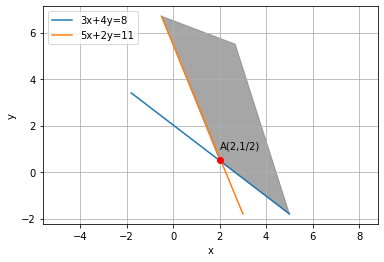
\includegraphics[width=\columnwidth]{solutions/su2021/2/12/Graphical Solution_10.png}
\caption{Graphical Solution}
\label{opt/12/fig:Graphical Solution}	
\end{figure}




\item One kind of cake requires 200g of flour and 25g of fat, and another kind of cake
requires 100g of flour and 50g of fat. Find the maximum number of cakes which
can be made from 5kg of flour and 1 kg of fat assuming that there is no shortage
of the other ingredients used in making the cakes.\\
\solution
We obtain the vertices of the rhombus as follows
\begin{align}
\vec{A} = \myvec{-3\\0},
\vec{B} = \myvec{0\\-3.5},
\vec{C} = \myvec{3\\0},
\vec{D} = \myvec{0\\3.5}
\end{align}
which are plotted in Fig. \ref{quad/45/fig:Rhombus ABCD}.
%
\begin{figure}[ht!]
\centering
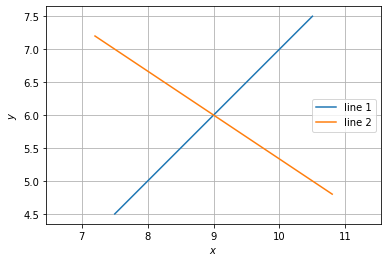
\includegraphics[width=\columnwidth]{solutions/quad/45/figure2.png}
\caption{Rhombus ABCD}
\label{quad/45/fig:Rhombus ABCD}
\end{figure}


\item A factory makes tennis rackets and cricket bats. A tennis racket takes 1.5 hours
of machine time and 3 hours of craftman’s time in its making while a cricket bat
takes 3 hour of machine time and 1 hour of craftman’s time. In a day, the factory
has the availability of not more than 42 hours of machine time and 24 hours of
craftsman’s time.\\
(i) What number of rackets and bats must be made if the factory is to work
at full capacity?\\
(ii)If the profit on a racket and on a bat is Rs 20 and Rs 10 respectively, find
the maximum profit of the factory when it works at full capacity.\\
\solution

\begin{table}[!ht]
\centering
\resizebox{\columnwidth}{!}{\begin{tabular}{|c|c|c|c|} 
\hline
item & Machine hours & Craftman's hours & profit \\
\hline
Tennis Racket & 1.5 & 3  &  20  \\ 
\hline
Cricket Bats & 3 & 1 &  10  \\ 
\hline
Maximum time Available & 42 & 24 & \\ 
\hline
\end{tabular}}
\caption{factory Requirements}
\label{opt/14/tab:table1}
\end{table}
Let the number of Tennis Rackets  be $x$ and the number of cricket bats be $y$  such that 
\begin{align}
x \geq 0 \\
y \geq 0 
\end{align}
According to the question,
\begin{align}
1.5x+3y &\leq 42 \\
\implies 3x+6y &\leq 84 \\
\implies x+2y &\leq 28 
\end{align}
and,
\begin{align}
3x+y &\leq 24 
\end{align}
$\therefore$ Our problem is
\begin{align}
\max_{\vec{x}} Z &= \myvec{20 & 10}\vec{x}\\
s.t. \quad \myvec{1 & 2 \\ 3 & 1}\vec{x} &\preceq \myvec{28\\24} 
\end{align}
Lagrangian function is given by
\begin{equation}
\begin{aligned}
&L(\vec{x},\boldsymbol{\lambda}) \\ &= \myvec{20 & 10}\vec{x}+\lcbrak{\sbrak{\myvec{1 & 2}\vec{x}-28}} \\ &+ \sbrak{\myvec{3 & 1}\vec{x}-24}\\ &+ \sbrak{\myvec{-1 & 0}\vec{x}} +\rcbrak{\sbrak{\myvec{0 & -1}\vec{x}}}\boldsymbol{\lambda}
\end{aligned}
\end{equation}
where,
\begin{align}
\boldsymbol{\lambda} &= \myvec{\lambda_1 \\ \lambda_2 \\ \lambda_3 \\ \lambda_4 \\ \lambda_5 \\ \lambda_6}
\end{align}
Now,
\begin{align}
\nabla L(\vec{x},\boldsymbol{\lambda}) &= \myvec{20+ \myvec{1 & 3  & -1 & 0 }\boldsymbol{\lambda}\\ 10+\myvec{2 & 1 & 0 & -1}\boldsymbol{\lambda} \\ \myvec{1 & 2}\vec{x}-28 \\ \myvec{3 & 1}\vec{x}-24 \\  \myvec{-1 & 0}\vec{x} \\ \myvec{0 & -1}\vec{x}}
\end{align}
$\therefore$ Lagrangian matrix is given by
\begin{align}
\myvec{0 & 0 & 1 & 3 & -1 & 0 \\ 0 & 0 & 2 & 1  & 0 & -1 \\ 1 & 2 & 0 & 0 & 0 & 0 \\ 3 & 1 & 0 & 0 & 0 & 0  \\ -1 & 0 & 0 & 0 & 0 & 0  \\ 0 & -1 & 0 & 0 & 0 & 0 }\myvec{\vec{x} \\ \boldsymbol{\lambda} } &= \myvec{-20 \\ -10 \\ 28 \\ 24 \\ 0 \\0 }
\end{align}
Considering $\lambda_1,\lambda_2$ as only active multiplier,
\begin{align}
\myvec{0 & 0 & 1 & 3 \\ 0 & 0 & 2 & 1 \\ 1 & 2 & 0 & 0 \\ 3 & 1 & 0 & 0}\myvec{\vec{x}\\ \boldsymbol{\lambda}} &= \myvec{-20 \\ -10 \\ 28 \\ 24}
\end{align}
resulting in,
\begin{align}
\myvec{\vec{x} \\ \boldsymbol{\lambda}} &= \myvec{0 & 0 & 1 & 3 \\ 0 & 0 & 2 & 1 \\ 1 & 2 & 0 & 0 \\ 3 & 1 & 0 & 0}^{-1}\myvec{-20 \\ -10 \\ 28 \\ 24}
\\
\implies   \myvec{\vec{x} \\ \boldsymbol{\lambda}} &= \myvec{0 & 0 & \frac{-1}{5} & \frac{2}{5} \\ 0 & 0 & \frac{3}{5} & \frac{-1}{5} \\ \frac{-1}{5} & \frac{3}{5} & 0 & 0 \\ \frac{2}{5} & \frac{-1}{5} & 0 & 0}\myvec{-20 \\ -10 \\ 28 \\ 24}
\\
\implies \myvec{\vec{x} \\ \boldsymbol{\lambda}} &= \myvec{4 \\ 12 \\ -2 \\ -6 }
\end{align}
$\because \boldsymbol{\lambda}=\myvec{-2 \\ -6} \succ \vec{0} $
\\
$\therefore$ Optimal solution is given by
\begin{align}
\vec{x} &= \myvec{4\\12} \\
Z &= \myvec{20 & 10}\vec{x} \\
&= \myvec{20 & 10}\myvec{4 \\ 12} \\
&= 200
\end{align}
By using cvxpy in python ,
\begin{align}
\vec{x}=\myvec{3.99999998\\12.0000000}\\
Z = 199.99999964
\end{align}
Hence ,\boxed{x=4} Tennis Rackets and \boxed{y=12} Cricket Bats should be used to maximum time Available profit \boxed{Z=200} as can be
verified from Fig. \ref{opt/14/fig: Graphical Solution}.	
\begin{enumerate}
\item 4 Tennis Rackets and 12 Cricket Bats must be made so that factory runs at full capacity.
\item Maximum profit is Rs 200, When 4 Tennis Bats and 12 Cricket Bats are produced.
\end{enumerate}
%
\begin{figure}[!ht]
\centering
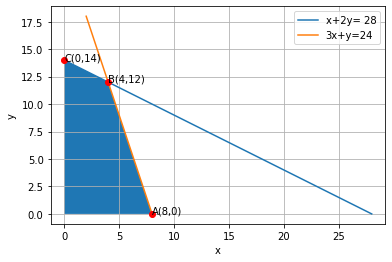
\includegraphics[width=\columnwidth]{solutions/su2021/2/14/download.png}
\caption{Graphical Solution}
\label{opt/14/fig: Graphical Solution}	
\end{figure}



\item A manufacturer produces nuts and bolts. It takes 1 hour of work on machine A
and 3 hours on machine B to produce a package of nuts. It takes 3 hours on
machine A and 1 hour on machine B to produce a package of bolts. He earns a
profit of Rs17.50 per package on nuts and Rs 7.00 per package on bolts. How
many packages of each should be produced each day so as to maximise his
profit, if he operates his machines for at the most 12 hours a day?\\
\solution
We obtain the vertices of the rhombus as follows
\begin{align}
\vec{A} = \myvec{-3\\0},
\vec{B} = \myvec{0\\-3.5},
\vec{C} = \myvec{3\\0},
\vec{D} = \myvec{0\\3.5}
\end{align}
which are plotted in Fig. \ref{quad/45/fig:Rhombus ABCD}.
%
\begin{figure}[ht!]
\centering
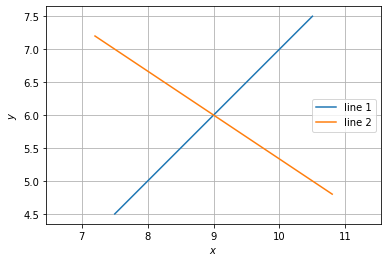
\includegraphics[width=\columnwidth]{solutions/quad/45/figure2.png}
\caption{Rhombus ABCD}
\label{quad/45/fig:Rhombus ABCD}
\end{figure}


\item A factory manufactures two types of screws, A and B. Each type of screw
requires the use of two machines, an automatic and a hand operated. It takes
4 minutes on the automatic and 6 minutes on hand operated machines to
manufacture a package of screws A, while it takes 6 minutes on automatic and
3 minutes on the hand operated machines to manufacture a package of screws
B. Each machine is available for at the most 4 hours on any day. The manufacturer
can sell a package of screws A at a profit of Rs 7 and screws B at a profit of
Rs 10. Assuming that he can sell all the screws he manufactures, how many
packages of each type should the factory owner produce in a day in order to
maximise his profit? Determine the maximum profit.\\
\solution

\begin{table}[!ht]
\centering
\resizebox{\columnwidth}{!}{\begin{tabular}{|c|c|c|c|c|} 
\hline
Item & Number & Machine A & Machine B & Profit \\
\hline
Screw A & x & 4 minutes & 6 minutes & Rs 7 \\
\hline
Screw B & y & 6 minutes & 3 minutes & Rs 10 
\\
\hline
Max Available Time &  & 4hours  =240minutes & 4hours =240minutes &
\\
\hline
\end{tabular}}
\caption{Screw Requirements}
\label{opt/16/tab:table1}
\end{table}
Let the number of packages of screw  A be $x$ and the number of packages of screw B be $y$  such that 
\begin{align}
    x \geq 0 \\
    y \geq 0 
\end{align}
According to the question,
\begin{align}
    4x+6y &\leq 240 \\
 \implies 2x+3y &\leq 120
\end{align}
     and,
\begin{align}
    6x+3y &\leq 240 \\
 \implies 2x+y &\leq 80
\end{align}
$\therefore$ Our problem is
\begin{align}
        \max_{\vec{x}} Z &= \myvec{7 & 10}\vec{x}\\
        s.t. \quad 
        \myvec{2 & 3 \\ 2 & 1 }\vec{x} &\preceq \myvec{120\\80} 
\end{align}
Lagrangian function is given by
\begin{equation}
\begin{aligned}
    &L(\vec{x},\boldsymbol{\lambda}) \\ &= \myvec{7 & 10}\vec{x}+\lcbrak{\sbrak{\myvec{2 & 3}\vec{x}+120}} \\ &+ \sbrak{\myvec{2 & 1}\vec{x}+80} \\ &+ \sbrak{\myvec{-1 & 0}\vec{x}} +\rcbrak{\sbrak{\myvec{0 & -1}\vec{x}}}\boldsymbol{\lambda}
\end{aligned}
\end{equation}
where,
\begin{align}
    \boldsymbol{\lambda} &= \myvec{\lambda_1 \\ \lambda_2 \\ \lambda_3 \\ \lambda_4 \\ \lambda_5 \\ \lambda_6}
\end{align}
Now,
\begin{align}
    \nabla L(\vec{x},\boldsymbol{\lambda}) &= \myvec{7+ \myvec{2 & 3 & -1 & 0 }\boldsymbol{\lambda}\\ 10+\myvec{2 & 1 & 0 & -1}\boldsymbol{\lambda} \\ \myvec{2 & 3}\vec{x}+120 \\ \myvec{2 & 1}\vec{x}+80 \\ \myvec{-1 & 0}\vec{x} \\ \myvec{0 & -1}\vec{x}}
\end{align}
$\therefore$ Lagrangian matrix is given by
\begin{align}
    \myvec{0 & 0 & 2 & 3 & -1 & 0 \\ 0 & 0 & 2 & 1 & 0 & -1 \\ 2 & 3 & 0 & 0 & 0 & 0  \\ 2 & 1 & 0 & 0 & 0 & 0  \\ -1 & 0 & 0 & 0 & 0 & 0  \\ 0 & -1 & 0 & 0 & 0 & 0 }\myvec{\vec{x} \\ \boldsymbol{\lambda} } &= \myvec{-5 \\ -6 \\ 200 \\ 240 \\ 0 \\0 }
\end{align}
Considering $\lambda_1,\lambda_2$ as only active multiplier,
\begin{align}
    \myvec{0 & 0 & 2 & 3 \\ 0 & 0 & 2 & 1 \\ 2 & 3 & 0 & 0 \\ 2 & 1 & 0 & 0}\myvec{\vec{x}\\ \boldsymbol{\lambda}} &=\myvec{-7 \\ -10 \\ 120 \\ 80}
\end{align}
resulting in,
\begin{align}
    \myvec{\vec{x} \\ \boldsymbol{\lambda}} &= \myvec{0 & 0 & 2 & 3 \\ 0 & 0 & 2 & 1 \\ 2 & 3 & 0 & 0 \\ 2 & 1 & 0 & 0}^{-1}\myvec{-7 \\ -10 \\ 120 \\ 80}
    \\
    \implies   \myvec{\vec{x} \\ \boldsymbol{\lambda}} &= \myvec{0 & 0 & \frac{-1}{4} & \frac{3}{4} \\ 0 & 0 & \frac{1}{2} & \frac{-1}{2} \\ \frac{-1}{4} & \frac{1}{2} & 0 & 0 \\ \frac{1}{2} & \frac{-1}{2} & 0 & 0}\myvec{-7 \\ -10 \\ 120 \\ 80}
    \\
    \implies \myvec{\vec{x} \\ \boldsymbol{\lambda}} &= \myvec{30 \\ 20 \\ \frac{-13}{4} \\ \frac{3}{2} }
\end{align}
$\because \boldsymbol{\lambda}=\myvec{\frac{-13}{4} \\ \frac{3}{2}} \succ \vec{0} $ 
\\
$\therefore$ Optimal solution is given by
\begin{align}
    \vec{x} &= \myvec{30\\20} \\
    Z &= \myvec{7 & 10}\vec{x} \\
    &= \myvec{7 & 10}\myvec{30 \\ 20} \\
    &= 410
\end{align}
By using cvxpy in python ,
\begin{align}
    \vec{x}=\myvec{30.00000000\\20.00000000}\\
    Z = 410.00000000
\end{align}
Hence ,\boxed{x=30} packages of screw A and \boxed{y=20} packages of screw B should be the factory owner produce in a day in order to maximise his  profit is \boxed{Z=410}.  This
is verified in Fig. \ref{opt/16/fig: graphical solution}.	
%
\begin{figure}[!ht]
\centering
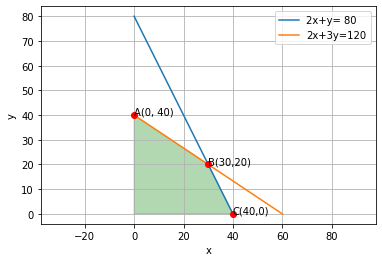
\includegraphics[width=\columnwidth]{solutions/su2021/2/16/Figure 11.png}
\caption{graphical solution}
\label{opt/16/fig: graphical solution}	
\end{figure}


\item A cottage industry manufactures pedestal lamps and wooden shades, each
requiring the use of a grinding/cutting machine and a sprayer. It takes 2 hours on
grinding/cutting machine and 3 hours on the sprayer to manufacture a pedestal
lamp. It takes 1 hour on the grinding/cutting machine and 2 hours on the sprayer
to manufacture a shade. On any day, the sprayer is available for at the most 20
hours and the grinding/cutting machine for at the most 12 hours. The profit from
the sale of a lamp is Rs 5 and that from a shade is Rs 3. Assuming that the
manufacturer can sell all the lamps and shades that he produces, how should he
schedule his daily production in order to maximise his profit?\\
\solution
We obtain the vertices of the rhombus as follows
\begin{align}
\vec{A} = \myvec{-3\\0},
\vec{B} = \myvec{0\\-3.5},
\vec{C} = \myvec{3\\0},
\vec{D} = \myvec{0\\3.5}
\end{align}
which are plotted in Fig. \ref{quad/45/fig:Rhombus ABCD}.
%
\begin{figure}[ht!]
\centering
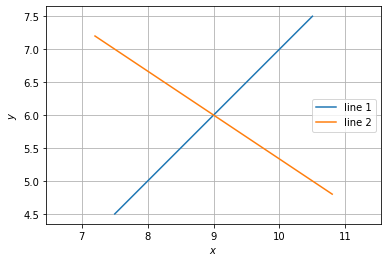
\includegraphics[width=\columnwidth]{solutions/quad/45/figure2.png}
\caption{Rhombus ABCD}
\label{quad/45/fig:Rhombus ABCD}
\end{figure}


\item A company manufactures two types of novelty souvenirs made of plywood.
Souvenirs of type A require 5 minutes each for cutting and 10 minutes each for
assembling. Souvenirs of type B require 8 minutes each for cutting and 8 minutes
each for assembling. There are 3 hours 20 minutes available for cutting and 4
hours for assembling. The profit is Rs 5 each for type A and Rs 6 each for type
B souvenirs. How many souvenirs of each type should the company manufacture
in order to maximise the profit?\\
\solution
We obtain the vertices of the rhombus as follows
\begin{align}
\vec{A} = \myvec{-3\\0},
\vec{B} = \myvec{0\\-3.5},
\vec{C} = \myvec{3\\0},
\vec{D} = \myvec{0\\3.5}
\end{align}
which are plotted in Fig. \ref{quad/45/fig:Rhombus ABCD}.
%
\begin{figure}[ht!]
\centering
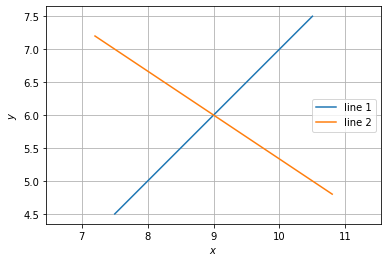
\includegraphics[width=\columnwidth]{solutions/quad/45/figure2.png}
\caption{Rhombus ABCD}
\label{quad/45/fig:Rhombus ABCD}
\end{figure}

\item A manufacturer makes two types of toys A and B. Three machines are needed
for this purpose and the time (in minutes) required for each toy on the machines
is given below:\\
\begin{table}[!ht]
    \begin{center}
    \begin{tabular}{|l|l|l|l|} \hline
    \multicolumn{4}{|c|} {Machines} \\ \hline
    Types of toys & I & II & III \\ \hline
    A & 12 & 18 & 6\\ \hline
    B & 6 & 0 & 9\\ \hline
    \end{tabular}
    \end{center}
    \caption{Toys table}
    \label{opt/26/opt/26/tab:table1}
    \end{table}


Each machine is available for a maximum of 6 hours per day. If the profit on
each toy of type A is Rs 7.50 and that on each toy of type B is Rs 5, show that 15
toys of type A and 30 of type B should be manufactured in a day to get maximum
profit.\\
\\
\solution 
We obtain the vertices of the rhombus as follows
\begin{align}
\vec{A} = \myvec{-3\\0},
\vec{B} = \myvec{0\\-3.5},
\vec{C} = \myvec{3\\0},
\vec{D} = \myvec{0\\3.5}
\end{align}
which are plotted in Fig. \ref{quad/45/fig:Rhombus ABCD}.
%
\begin{figure}[ht!]
\centering
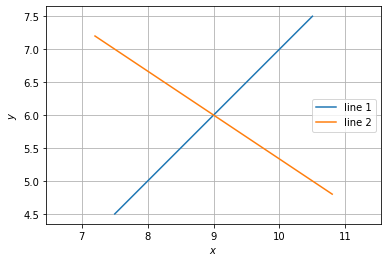
\includegraphics[width=\columnwidth]{solutions/quad/45/figure2.png}
\caption{Rhombus ABCD}
\label{quad/45/fig:Rhombus ABCD}
\end{figure}


\item Two godowns A and B have grain capacity of 100 quintals and 50 quintals respectively.They supply to 3 ration shops, D, E and F whose requirements are 60, 50 and 40 quintals respectively. The cost of transportation per quintal from the godowns to the shops are given in the following table:
\numberwithin{table}{section}
\begin{table}[!ht]
\begin{center}
\begin{tabular}{ |l|l|l|}
\hline
\multicolumn{3}{ |c| }{Transportation cost per quintal (in rupees)} \\
\hline
From/To & A & B \\ \hline
D & 6 & 4  \\ \hline
E & 3 & 2 \\ \hline
F & 2.50 & 3 \\ \hline
\end{tabular}
\end{center}
\caption{Transportation table}
\label{opt/28/tab:table1}
\end{table}
How should the supplies be transported in order that the transportation cost is minimum? What is the minimum cost?
\\
\solution 
\input{solutions/su2021/2/28/Assignment-12.tex}
\item A fruit grower can use two types of fertilizer in his garden, brand P and brand Q.The amounts(in kg) of nitrogen, phosphoric acid,potash and chlorine in a bag of each brand are given in the table.Tests indicate that garden needs atleast 240 kg of phosphoric acid,atleast 270 kg of potash and atmost 310 kg of chlorine. If the grower wants to minimise the amount of nitrogen added to garden, how many bags of each brand should be used?What is the minimum amount of nitrogen added in the ground?

\begin{table}[!ht]
\centering
\resizebox{\columnwidth}{!}{\begin{tabular}{|c|c|c|} 
\hline
 & \textbf{Brand P }& \textbf{Brand Q }\\
\hline
Nitrogen & 3  & 3.5  \\ 
\hline
Phosphoric Acid & 1 & 2 \\ 
\hline
Potash & 3 & 1.5\\ 
\hline
Chlorine & 1.5 & 2 \\ 
\hline
\end{tabular}}
\caption{kg per bag}
\label{opt/30/tab:table1}
\end{table}
%
\solution
\begin{itemize}
\item All the data can be tabularised as:
\numberwithin{table}{section}
\begin{table}[!ht]
\centering
\resizebox{\columnwidth}{!}{\begin{tabular}{|c|c|c|c|} 
\hline
 & \textbf{Brand P }& \textbf{Brand Q } &Amounts Required\\
\hline
Nitrogen & 3  & 3.5 & $?$ \\ 
\hline
Phosphoric Acid & 1 & 2 &$\geq 240$ kg \\ 
\hline
Potash & 3 & 1.5 &$\geq 270$ kg\\ 
\hline
Chlorine & 1.5 & 2 &$\leq 310$ kg\\ 
\hline
\end{tabular}}
\caption{Requirements of fertilizers}
\label{opt/30/tab:table2}
\end{table}
\item Let the number of bags of Brand P be $x$ $\And$
\item The number of bags of Brand Q be $y$ such that : 
\begin{align}
    x \geq 0 
    \\
    y \geq 0 
\end{align}
\item From the data given we have:
\begin{align}
    x+2y &\geq 240 \\
   \implies   -x-2y &\leq -240
\end{align}
and,
\begin{align}
    3x+1.5y &\geq 270 \\
    \implies -x-0.5y &\leq -90
\end{align}
and,
\begin{align}
     1.5x+2y &\leq 310 \\
\end{align}
$\therefore$ The minimizing function is:
\begin{align}
        \min_{\vec{x}} Z &= \myvec{3& 3.5}\vec{x}\\
        s.t. \quad 
        \myvec{-1 & -2\\ -1 & -0.5 \\ 1.5 & 2 }\vec{x} &\preceq \myvec{-240\\-90\\310} \\
        \vec{-x} &\preceq \vec{0}
\end{align}
\item The Lagrangian function can be given as:
\begin{equation}
\begin{aligned}
    &L(\vec{x},\boldsymbol{\lambda}) \\ &= \myvec{3 & 3.5}\vec{x}+\lcbrak{\sbrak{\myvec{-1 & -2}\vec{x}+240}} \\ &+ \sbrak{\myvec{-1 & -0.5}\vec{x}+90} +\sbrak{\myvec{1.5 & 2}\vec{x}-310} \\ &+ \sbrak{\myvec{-1 & 0}\vec{x}} +\rcbrak{\sbrak{\myvec{0 & -1}\vec{x}}}\boldsymbol{\lambda}
\end{aligned}
\end{equation}
where,
\begin{align}
    \boldsymbol{\lambda} &= \myvec{\lambda_1 \\ \lambda_2 \\ \lambda_3 \\ \lambda_4 \\ \lambda_5 \\ \lambda_6}
\end{align}
\item Now, we have
\begin{align}
    \nabla L(\vec{x},\boldsymbol{\lambda}) &= \myvec{3+ \myvec{-1 & -1 & 1.5 & -1 & 0 }\boldsymbol{\lambda}\\ 3.5+\myvec{-2 & -0.5 & 2 & 0 & -1}\boldsymbol{\lambda} \\ \myvec{-1 & -2}\vec{x}+240 \\ \myvec{-1 & -0.5}\vec{x}+90 \\ \myvec{1.5 & 2}\vec{x}-310 \\ \myvec{-1 & 0}\vec{x} \\ \myvec{0 & -1}\vec{x}}
\end{align}
$\therefore$ The Lagrangian matrix is given by:-
\begin{align}
  \small{\myvec{0 & 0 & -1 & -1 & 1.5 & -1 & 0 \\ 0 & 0 & -2 & -0.5 & 2 & 0 & -1 \\ -1 & -2 & 0 & 0 & 0 & 0 & 0 \\ -1 & -0.5 & 0 & 0 & 0 & 0 & 0 \\ 1.5 & 2 & 0 & 0 & 0 & 0 & 0 \\ -1 & 0 & 0 & 0 & 0 & 0 & 0 \\ 0 & -1 & 0 & 0 & 0 & 0 & 0 }\myvec{\vec{x} \\ \boldsymbol{\lambda} }}= \small{\myvec{-3 \\ -3.5 \\ -240 \\ -90 \\ 310 \\ 0 \\0 }}
\end{align}
\item Considering $\lambda_1,\lambda_2$ as only active multiplier,
\begin{align}
    \myvec{0 & 0 & -1 & -1  \\ 0 & 0 & -2 & -0.5 \\ -1 & -2 & 0 & 0 \\-1 & -0.5 & 0 & 0}\myvec{\vec{x}\\ \boldsymbol{\lambda}} &= \myvec{-3 \\ -3.5 \\ -240 \\ -90}
\end{align}
\begin{align}
 \implies   \myvec{\vec{x} \\ \boldsymbol{\lambda}} &=  \myvec{0 & 0 & -1 & -1  \\ 0 & 0 & -2 & -0.5 \\ -1 & -2 & 0 & 0 \\-1 & -0.5 & 0 & 0}^{-1}\myvec{-3 \\ -3.5 \\ -240 \\ -90}
    \\
    \implies   \myvec{\vec{x} \\ \boldsymbol{\lambda}} &= \myvec{0 & 0 & \frac{1}{3} & \frac{4}{3} \\ 0 & 0 & \frac{-2}{3} & \frac{2}{3} \\ \frac{1}{3} & \frac{-2}{3} & 0 & 0 \\ \frac{-4}{3} & \frac{2}{3} & 0 & 0}\myvec{-3 \\ -3.5 \\ -240 \\ -90}
    \\
    \implies \myvec{\vec{x} \\ \boldsymbol{\lambda}} &= \myvec{40 \\100 \\ \frac{4}{3} \\ \frac{5}{3} }
\end{align}
$\because \boldsymbol{\lambda}=\myvec{\frac{4}{3} \\ \frac{5}{3}} \succ \vec{0}$
\\
\item The Optimal solution is given by:
\begin{align}
    \vec{x} &= \myvec{40\\100} \\
    Z &= \myvec{3&3.5}\vec{x} \\
   Z &= \myvec{3&3.5}\myvec{40 \\ 100} \\
    Z&= 470 \text{ units}
\end{align}
\item So, we get
\\
 Bags of brand \textbf{P} as \boxed{x=40} $\And$
 \\
 Bags of brand \textbf{Q} as  \boxed{y=100} so as to minimise the amount of nitrogen added.
\item The minimum amount of nitrogen required is \boxed{Z=470 \text{ units}} .  Fig. \ref{opt/30/fig}
verifies this result.
%
\begin{figure}[!ht]
\centering
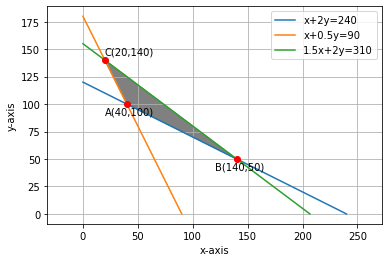
\includegraphics[width=\columnwidth]{solutions/su2021/2/30/Graphical_Solution_2.30.png}
\caption{Graphical Solution}
\label{opt/30/fig}
\end{figure}

\end{itemize}


\item A toy company manufactures two types of dolls, A and B. Market research and
available resources have indicated that the combined production level should not
exceed 1200 dolls per week and the demand for dolls of type B is at most half of that
for dolls of type A. Further, the production level of dolls of type A can exceed three
times the production of dolls of other type by at most 600 units. If the company
makes profit of Rs 12 and Rs 16 per doll respectively on dolls A and B, how many of
each should be produced weekly in order to maximise the profit?
%
\solution
We obtain the vertices of the rhombus as follows
\begin{align}
\vec{A} = \myvec{-3\\0},
\vec{B} = \myvec{0\\-3.5},
\vec{C} = \myvec{3\\0},
\vec{D} = \myvec{0\\3.5}
\end{align}
which are plotted in Fig. \ref{quad/45/fig:Rhombus ABCD}.
%
\begin{figure}[ht!]
\centering
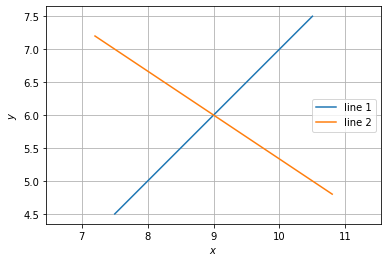
\includegraphics[width=\columnwidth]{solutions/quad/45/figure2.png}
\caption{Rhombus ABCD}
\label{quad/45/fig:Rhombus ABCD}
\end{figure}


\item  \textbf{(Manufacturing problem)} A manufacturing company makes two models
A and B of a product. Each piece of Model A requires 9 labour hours for fabricating
and 1 labour hour for finishing. Each piece of Model B requires 12 labour hours for
fabricating and 3 labour hours for finishing. For fabricating and finishing, the maximum
labour hours available are 180 and 30 respectively. The company makes a profit of
Rs 8000 on each piece of model A and Rs 12000 on each piece of Model B. How many
pieces of Model A and Model B should be manufactured per week to realise a maximum
profit? What is the maximum profit per week?\\
\solution
\begin{itemize}
\item All the data can be tabularised as:
%
\begin{table}[!ht]
\centering
\resizebox{\columnwidth}{!}{\begin{tabular}{|c|c|c|c|} 
\hline
 & Fabricating&Finishing &Profit\\
\hline
\textbf{Model A} & 9  & 1 & 8000 \\ 
\hline
\textbf{Model B} & 12  & 3 & 12000 \\ 
\hline
\text{Max Hours} & $\leq180$&$\leq30$&\\
\hline
\end{tabular}}
\caption{Labour Hours and Profit for each piece}
\label{opt/2/35/tab:table1}
\end{table}
\item Let the number of pieces of model A manufactured be $x$ and
the number of pieces of model B manufactured be $y$ such that : 
\begin{align}
    x \geq 0 
    \\
    y \geq 0 
\end{align}
\item From the data given we have:
\begin{align}
    9x+12y &\leq 180 \\
    \implies 3x+4y&\leq60
\end{align}
and,
\begin{align}
    x+3y &\leq 30 
\end{align}

$\therefore$ The maximizing function is:
\begin{align}
        \max Z &= \myvec{8000& 12000}\vec{x}\\
        s.t. \quad 
        \myvec{3 & 4\\ 1 & 3 }\vec{x} &\preceq \myvec{60\\30} \\
        \vec{-x} &\preceq \vec{0}
\end{align}
\item The Lagrangian function can be given as:
\begin{equation}
\begin{aligned}
    &L(\vec{x},\boldsymbol{\lambda}) \\ &= \myvec{8000 & 12000}\vec{x}+\lcbrak{\sbrak{\myvec{3 & 4}\vec{x}-60}} \\ &+ \sbrak{\myvec{1 & 3}\vec{x}-30} \\ &+ \sbrak{\myvec{-1 & 0}\vec{x}} +\rcbrak{\sbrak{\myvec{0 & -1}\vec{x}}}\boldsymbol{\lambda}
\end{aligned}
\end{equation}
where,
\begin{align}
    \boldsymbol{\lambda} &= \myvec{\lambda_1 \\ \lambda_2 \\ \lambda_3 \\ \lambda_4}
\end{align}
\item Now, we have
\begin{align}
    \nabla L(\vec{x},\boldsymbol{\lambda}) &= \myvec{8000+ \myvec{3 & 1 & -1 & 0 }\boldsymbol{\lambda}\\ 12000+\myvec{4 & 3 &0 & -1}\boldsymbol{\lambda} \\ \myvec{3 & 4}\vec{x}-60 \\ \myvec{1 & 3}\vec{x}-30 \\ \myvec{-1 & 0}\vec{x} \\ \myvec{0 & -1}\vec{x}}
\end{align}
$\therefore$ The Lagrangian matrix is given by:-
\begin{align}
  \small{\myvec{0 & 0 & 3 & 1 & -1 & 0 \\ 0 & 0 & 4 & 3 &0 & -1 \\ 3 & 4 & 0 & 0 & 0 & 0 \\ 1 & 3 & 0 & 0 & 0 & 0 \\ -1 & 0 & 0 & 0 & 0 & 0 \\ 0 & -1 & 0 & 0 & 0 & 0 }\myvec{\vec{x} \\ \boldsymbol{\lambda} }}= \small{\myvec{-8000 \\ -12000 \\ 60 \\ 30 \\ 0 \\0 }}
\end{align}
\item Considering $\lambda_1,\lambda_2$ as only active multiplier,
\begin{align}
    \myvec{0 & 0 & 3 & 1  \\ 0 & 0 & 4 & 3 \\ 3 & 4 & 0 & 0 \\1 & 3 & 0 & 0}\myvec{\vec{x}\\ \boldsymbol{\lambda}} &= \myvec{-8000 \\ -12000 \\ 60 \\ 30}
\end{align}
\begin{align}
 \implies   \myvec{\vec{x} \\ \boldsymbol{\lambda}} &=  \myvec{0 & 0 & 3 & 1  \\ 0 & 0 & 4 & 3 \\ 3 & 4 & 0 & 0 \\1 & 3 & 0 & 0} ^{-1}\myvec{-8000 \\ -12000 \\ 60 \\ 30}
    \\
    \implies   \myvec{\vec{x} \\ \boldsymbol{\lambda}} &= \myvec{0 & 0 & \frac{3}{5} & \frac{-4}{5} \\ 0 & 0 & \frac{-1}{5} & \frac{3}{5} \\ \frac{3}{5} & \frac{-1}{5} & 0 & 0 \\ \frac{-4}{5} & \frac{3}{5} & 0 & 0}\myvec{-8000 \\ -12000 \\ 60 \\ 30}
    \\
    \implies \myvec{\vec{x} \\ \boldsymbol{\lambda}} &= \myvec{12 \\6 \\ -2400 \\ -800 }
\end{align}
$\because \boldsymbol{\lambda}=\myvec{-2400 \\ -800} \prec \vec{0}$
\\
\item The Optimal solution is given by:
\begin{align}
    \vec{x} &= \myvec{12\\6} \\
    Z &= \myvec{8000&12000}\vec{x} \\
   Z &= \myvec{8000&12000}\myvec{12 \\ 6} \\
    Z&= \text{Rs} 168000
\end{align}
\item So, to maximise profit
\\
 Pieces of model \textbf{A} manufactured is \boxed{x=12} and
 \\
  Pieces of model \textbf{B} manufactured is \boxed{y=6}.
\item The maximum profit per week is \boxed{Z=\text{Rs} 168000} .

\begin{figure}[!ht]
\centering
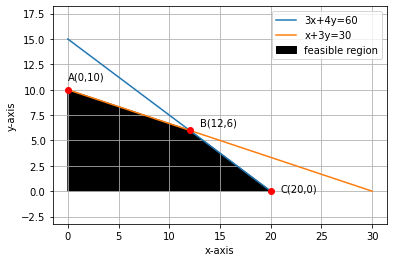
\includegraphics[width=\columnwidth]{solutions/su2021/2/35/Figure 10_1.png}
\caption{Graphical Representataion}
\end{figure}
\end{itemize}


\item \textbf {(Diet problem)} A dietician has to develop a special diet using two foods
P and Q. Each packet (containing 30 g) of food P contains 12 units of calcium, 4 units
of iron, 6 units of cholesterol and 6 units of vitamin A. Each packet of the same quantity
of food Q contains 3 units of calcium, 20 units of iron, 4 units of cholesterol and 3 units
of vitamin A. The diet requires atleast 240 units of calcium, atleast 460 units of iron and
at most 300 units of cholesterol. How many packets of each food should be used to
minimise the amount of vitamin A in the diet? What is the minimum amount of vitamin A?\\
\\
\solution
\begin{table}[!ht]
    \centering
    \resizebox{\columnwidth}{!}{\begin{tabular}{|c|c|c|c|} 
    \hline
    Component & P & Q & Requirement \\
    \hline
    Calcium & 12 units & 3 units & $\geq 240$ units \\ 
    \hline
    Iron & 4 units & 20 units & $\geq 460$ units \\ 
    \hline
    Cholesterol & 6 units & 4 units & $\leq 300$ units\\ 
    \hline
    Vitamin A & 6 units & 3 units & \\ 
    \hline
    \end{tabular}}
    \caption{Diet Requirements}
    \label{opt/36/tab:table1}
    \end{table}
    Let the number of packets of food P be $x$ and the number of packets of food Q be $y$  such that 
    \begin{align}
        x \geq 0 \\
        y \geq 0 
    \end{align}
    According to the question,
    \begin{align}
        12x+3y &\geq 240 \\
        \implies -4x-y &\leq -80 \\
    \end{align}
    and,
    \begin{align}
        4x+20y &\geq 460 \\
        \implies -x-5y &\leq -115 
    \end{align}
    and,
    \begin{align}
         6x+4y &\leq 300 \\
        \implies 3x+2y &\leq 150 
    \end{align}
    $\therefore$ Our problem is
    \begin{align}
            \min_{\vec{x}} Z &= \myvec{6 & 3}\vec{x}\\
            s.t. \quad 
            \myvec{-4 & -1 \\ -1 & -5 \\ 3 & 2 }\vec{x} &\preceq \myvec{-80\\-115\\150} \\
            \vec{-x} &\preceq \vec{0}
    \end{align}
    Lagrangian function is given by
    \begin{equation}
    \begin{aligned}
        &L(\vec{x},\boldsymbol{\lambda}) \\ &= \myvec{6 & 3}\vec{x}+\lcbrak{\sbrak{\myvec{-4 & -1}\vec{x}+80}} \\ &+ \sbrak{\myvec{-1 & -5}\vec{x}+115} +\sbrak{\myvec{3 & 2}\vec{x}-150} \\ &+ \sbrak{\myvec{-1 & 0}\vec{x}} +\rcbrak{\sbrak{\myvec{0 & -1}\vec{x}}}\boldsymbol{\lambda}
    \end{aligned}
    \end{equation}
    where,
    \begin{align}
        \boldsymbol{\lambda} &= \myvec{\lambda_1 \\ \lambda_2 \\ \lambda_3 \\ \lambda_4 \\ \lambda_5 \\ \lambda_6}
    \end{align}
    Now,
    \begin{align}
        \nabla L(\vec{x},\boldsymbol{\lambda}) &= \myvec{6+ \myvec{-4 & -1 & 3 & -1 & 0 }\boldsymbol{\lambda}\\ 3+\myvec{-1 & -5 & 2 & 0 & -1}\boldsymbol{\lambda} \\ \myvec{-4 & -1}\vec{x}+80 \\ \myvec{-1 & -5}\vec{x}+115 \\ \myvec{3 & 2}\vec{x}-150 \\ \myvec{-1 & 0}\vec{x} \\ \myvec{0 & -1}\vec{x}}
    \end{align}
    $\therefore$ Lagrangian matrix is given by
    \begin{align}
        \myvec{0 & 0 & -4 & -1 & 3 & -1 & 0 \\ 0 & 0 & -1 & -5 & 2 & 0 & -1 \\ -4 & -1 & 0 & 0 & 0 & 0 & 0 \\ -1 & -5 & 0 & 0 & 0 & 0 & 0 \\ 3 & 2 & 0 & 0 & 0 & 0 & 0 \\ -1 & 0 & 0 & 0 & 0 & 0 & 0 \\ 0 & -1 & 0 & 0 & 0 & 0 & 0 }\myvec{\vec{x} \\ \boldsymbol{\lambda} } &= \myvec{-6 \\ -3 \\ -80 \\ -115 \\ 150 \\ 0 \\0 }
    \end{align}
    Considering $\lambda_1,\lambda_2$ as only active multiplier,
    \begin{align}
        \myvec{0 & 0 & -4 & -1 \\ 0 & 0 & -1 & -5 \\ -4 & -1 & 0 & 0 \\ -1 & -5 & 0 & 0}\myvec{\vec{x}\\ \boldsymbol{\lambda}} &= \myvec{-6 \\ -3 \\ -80 \\ -115}
    \end{align}
    resulting in,
    \begin{align}
        \myvec{\vec{x} \\ \boldsymbol{\lambda}} &= \myvec{0 & 0 & -4 & -1 \\ 0 & 0 & -1 & -5 \\ -4 & -1 & 0 & 0 \\ -1 & -5 & 0 & 0}^{-1}\myvec{-6 \\ -3 \\ -80 \\ -115}
        \\
        \implies   \myvec{\vec{x} \\ \boldsymbol{\lambda}} &= \myvec{0 & 0 & \frac{-5}{19} & \frac{1}{19} \\ 0 & 0 & \frac{1}{19} & \frac{-4}{19} \\ \frac{-5}{19} & \frac{1}{19} & 0 & 0 \\ \frac{1}{19} & \frac{-4}{19} & 0 & 0}\myvec{-6 \\ -3 \\ -80 \\ -115}
        \\
        \implies \myvec{\vec{x} \\ \boldsymbol{\lambda}} &= \myvec{15 \\ 20 \\ \frac{27}{19} \\ \frac{6}{19} }
    \end{align}
    $\because \boldsymbol{\lambda}=\myvec{\frac{27}{19} \\ \frac{6}{19}} \succ \vec{0} $
    \\
    $\therefore$ Optimal solution is given by
    \begin{align}
        \vec{x} &= \myvec{15\\20} \\
        Z &= \myvec{6 & 3}\vec{x} \\
        &= \myvec{6 & 3}\myvec{15 \\ 20} \\
        &= 150
    \end{align}
    By using cvxpy in python ,
    \begin{align}
        \vec{x}=\myvec{14.99999999\\20.00000001}\\
        Z = 150.00000001
    \end{align}
    Hence ,\boxed{x=15} packets of food P and \boxed{y=20} packets of food Q should be used to minimise the amount of vitamin A in the diet and the minimum amount of vitamin A is \boxed{Z=150} units.  This is verified in Fig. \ref{opt/36/fig:diet problem}	
    %
    \begin{figure}[!ht]
    \centering
    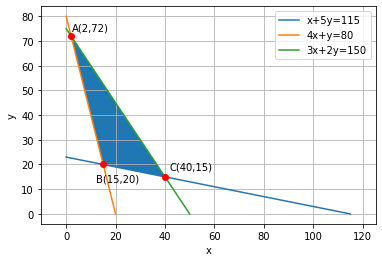
\includegraphics[width=\columnwidth]{solutions/su2021/2/36/Figure12.png}
    \caption{Diet Problem}
    \label{opt/36/fig:diet problem}	
    \end{figure}

%\end{enumerate}
%\end{document}

\end{enumerate}

\section{Gradient Descent}
\renewcommand{\theequation}{\theenumi}
\begin{enumerate}[label=\thesection.\arabic*.,ref=\thesection.\theenumi]
%\renewcommand{\theequation}{\theenumi}
%\begin{enumerate}[label=\thesubsection.\arabic*.,ref=\thesubsection.\theenumi]
%%\begin{enumerate}[label=\arabic*.,ref=\thesubsection.\theenumi]
%\numberwithin{equation}{enumi}
%

\item Find the absolute maximum and absoute minimum value of the following functions in the given intervals
%
\begin{enumerate}
\item $f(x) = 4x - \frac{1}{2}x^2, x \in \brak{-2,\frac{9}{2}}$
\item $f(x) = \brak{x-1}^2 + 3,  x \in \brak{-3,1}$
\end{enumerate}
%
\item Find the maximum profit that a company can make, if the profit function is given by
\begin{align}
p(x) = 41-72x - 18x^2
\end{align}
%
\item Find two positive numbers whose sum is 15 and the sum of whose squares is minimum.
\item Find two numbers whose sum is 24 and whose product is as large as possible.
\item Find two positive numbers whose sum is 16 and the sum of whose cubes is minimum.
\item The sum of the perimeter of a circle and square is $k$, where $k$ is some constant. Prove that the sum of their areas is least when the side of square is double the radius of the circle.
\item A window is in the form of a rectangle surmounted by a semicircular opening. The total perimeter of the window is 10 m. Find the dimensions of the window to admit maximum light through the whole opening.

\item Find the shortest distance of the point $\myvec{0\\c}$ from the parabola $y = x^2$, where $\frac{1}{2} \le c \le 5$.
\item Find the maximum area of an isosceles triangle inscribed in the ellipse 
%
\begin{align}
\vec{x}^T\myvec{a^2 & 0 \\ 0 & b^2}\vec{x} = a^2b^2
\end{align}
%
with its vertex at one end of the major axis.
\item Maximise Z=-x+2y, subject to the constraints:
x$\geq$3, x+y$\geq$5, x+2y$\geq$6, y$\geq$0.\\
\item Maximise Z=x+y, subject to x-y$\leq$-1,-x+y$\leq$0, x,y$\geq$0.\\
\item Reshma wishes to mix two types of food P and Q in such a way that the vitamin
contents of the mixture contain at least 8 units of vitamin A and 11 units of
vitamin B. Food P costs Rs 60/kg and Food Q costs Rs 80/kg. Food P contains
3 units/kg of Vitamin A and 5 units/kg of Vitamin B while food Q contains
4 units/kg of Vitamin A and 2 units/kg of vitamin B. Determine the minimum cost
of the mixture.\\
\solution

\begin{table}[!ht]
\centering
\resizebox{\columnwidth}{!}{\begin{tabular}{|c|c|c|c|} 
\hline
Food & Vitamin A & Vitamin B & Cost \\
\hline
P & 3 units/kg & 5 units/kg & 60 Rs/kg \\ 
\hline
Q & 4 units/kg & 2 units/kg & 80 Rs/kg \\ 
\hline
Requirement & 8 units/kg & 11 units/kg & \\ 
\hline
\end{tabular}}
\caption{Food Requirements}
\label{opt/12/tab:table1}
\end{table}
Let the mixture contain $x$ kg of food P and $y$ kg of food Q be $y$  such that 
\begin{align}
    x \geq 0 \\
    y \geq 0 
\end{align}
According to the question,
\begin{align}
    3x+4y &\geq 8 \\
    5x+2y &\geq 11
\end{align}
$\therefore$ Our problem is
\begin{align}
        \min_{\vec{x}} Z &= \myvec{60 & 80}\vec{x}\\
        s.t. \quad 
        \myvec{3 & 4 \\ 5 & 2 }\vec{x} &\preceq \myvec{8\\11} \\
        \vec{x} &\preceq \vec{0}
\end{align}
Lagrangian function is given by
\begin{equation}
\begin{aligned}
    &L(\vec{x},\boldsymbol{\lambda}) \\ &= \myvec{60 & 80}\vec{x}+\lcbrak{\sbrak{\myvec{3 & 4}\vec{x}-8}} \\ &+ \sbrak{\myvec{5 & 2}\vec{x}-11} \\ &+ \sbrak{\myvec{-1 & 0}\vec{x}} +\rcbrak{\sbrak{\myvec{0 & -1}\vec{x}}}\boldsymbol{\lambda}
\end{aligned}
\end{equation}
where,
\begin{align}
    \boldsymbol{\lambda} &= \myvec{\lambda_1 \\ \lambda_2 \\ \lambda_3 \\ \lambda_4}
\end{align}
Now,
\begin{align}
    \nabla L(\vec{x},\boldsymbol{\lambda}) &= \myvec{60+ \myvec{3 & 5 & -1 & 0 }\boldsymbol{\lambda}\\ 80+\myvec{4 & 2 & 0 & -1}\boldsymbol{\lambda} \\ \myvec{3 & 4}\vec{x}-8 \\ \myvec{5 & 2}\vec{x}-11 \\ \myvec{-1 & 0}\vec{x} \\ \myvec{0 & -1}\vec{x}}
\end{align}
$\therefore$ Lagrangian matrix is given by
\begin{align}
    \myvec{0 & 0 & 3 & 5 & -1 & 0 \\ 0 & 0 & 4 & 2 & 0 & -1 \\ 3 & 4 & 0 & 0 & 0 & 0 \\ 5 & 2 & 0 & 0 & 0 & 0 \\ -1 & 0 & 0 & 0 & 0 & 0 \\ 0 & -1 & 0 & 0 & 0 & 0}\myvec{\vec{x} \\ \boldsymbol{\lambda} } &= \myvec{-60 \\ -80 \\ 8 \\ 11 \\ 0 \\0 }
\end{align}
Considering $\lambda_1,\lambda_2$ as only active multiplier,
\begin{align}
    \myvec{0 & 0 & 3 & 5 \\ 0 & 0 & 4 & 2 \\ 3 & 4 & 0 & 0 \\ 5 & 2 & 0 & 0}\myvec{\vec{x}\\ \boldsymbol{\lambda}} &= \myvec{-60 \\ -80 \\ 8 \\ 11}
\end{align}
resulting in,
\begin{align}
    \myvec{\vec{x} \\ \boldsymbol{\lambda}} &= \myvec{0 & 0 & 3 & 5 \\ 0 & 0 & 4 & 2 \\ 3 & 4 & 0 & 0 \\ 5 & 2 & 0 & 0}^{-1}\myvec{-60 \\-80 \\ 8 \\ 11}
    \\
    \implies   \myvec{\vec{x} \\ \boldsymbol{\lambda}} &= \myvec{0 & 0 & \frac{-28}{196} & \frac{56}{196} \\ 0 & 0 & \frac{70}{196} & \frac{-42}{196} \\ \frac{-28}{196} & \frac{70}{196} & 0 & 0 \\ \frac{56}{196} & \frac{-42}{196} & 0 & 0}\myvec{-60 \\-80 \\ 8 \\ 11}
    \\
    \implies \myvec{\vec{x} \\ \boldsymbol{\lambda}} &= \myvec{2 \\ \frac{1}{2} \\ -20 \\ 0 }
\end{align}
$\because \boldsymbol{\lambda}=\myvec{-20 \\ 0} \preceq \vec{0} $
\\
$\therefore$ Optimal solution is given by
\begin{align}
    \vec{x} &= \myvec{2\\ \frac{1}{2}} \\
    Z &= \myvec{60 & 80}\vec{x} \\
    &= \myvec{60 & 80}\myvec{2 \\ \frac{1}{2}} \\
    &= 160
\end{align}
By using cvxpy in python,
\begin{align}
    \vec{x}=\myvec{2.11436237\\0.41422822}\\
    Z = 159.99999999
\end{align}
Fig. \ref{opt/12/fig:Graphical Solution}	verifies this result.
%
\begin{figure}[!ht]
\centering
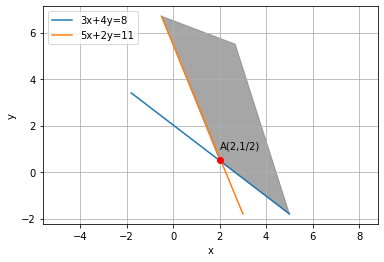
\includegraphics[width=\columnwidth]{solutions/su2021/2/12/Graphical Solution_10.png}
\caption{Graphical Solution}
\label{opt/12/fig:Graphical Solution}	
\end{figure}




\item One kind of cake requires 200g of flour and 25g of fat, and another kind of cake
requires 100g of flour and 50g of fat. Find the maximum number of cakes which
can be made from 5kg of flour and 1 kg of fat assuming that there is no shortage
of the other ingredients used in making the cakes.\\
\solution
We obtain the vertices of the rhombus as follows
\begin{align}
\vec{A} = \myvec{-3\\0},
\vec{B} = \myvec{0\\-3.5},
\vec{C} = \myvec{3\\0},
\vec{D} = \myvec{0\\3.5}
\end{align}
which are plotted in Fig. \ref{quad/45/fig:Rhombus ABCD}.
%
\begin{figure}[ht!]
\centering
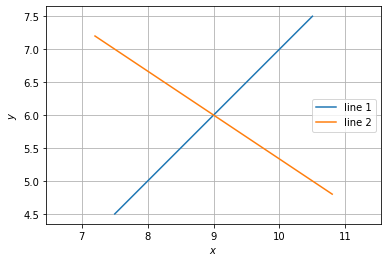
\includegraphics[width=\columnwidth]{solutions/quad/45/figure2.png}
\caption{Rhombus ABCD}
\label{quad/45/fig:Rhombus ABCD}
\end{figure}


\item A factory makes tennis rackets and cricket bats. A tennis racket takes 1.5 hours
of machine time and 3 hours of craftman’s time in its making while a cricket bat
takes 3 hour of machine time and 1 hour of craftman’s time. In a day, the factory
has the availability of not more than 42 hours of machine time and 24 hours of
craftsman’s time.\\
(i) What number of rackets and bats must be made if the factory is to work
at full capacity?\\
(ii)If the profit on a racket and on a bat is Rs 20 and Rs 10 respectively, find
the maximum profit of the factory when it works at full capacity.\\
\solution

\begin{table}[!ht]
\centering
\resizebox{\columnwidth}{!}{\begin{tabular}{|c|c|c|c|} 
\hline
item & Machine hours & Craftman's hours & profit \\
\hline
Tennis Racket & 1.5 & 3  &  20  \\ 
\hline
Cricket Bats & 3 & 1 &  10  \\ 
\hline
Maximum time Available & 42 & 24 & \\ 
\hline
\end{tabular}}
\caption{factory Requirements}
\label{opt/14/tab:table1}
\end{table}
Let the number of Tennis Rackets  be $x$ and the number of cricket bats be $y$  such that 
\begin{align}
x \geq 0 \\
y \geq 0 
\end{align}
According to the question,
\begin{align}
1.5x+3y &\leq 42 \\
\implies 3x+6y &\leq 84 \\
\implies x+2y &\leq 28 
\end{align}
and,
\begin{align}
3x+y &\leq 24 
\end{align}
$\therefore$ Our problem is
\begin{align}
\max_{\vec{x}} Z &= \myvec{20 & 10}\vec{x}\\
s.t. \quad \myvec{1 & 2 \\ 3 & 1}\vec{x} &\preceq \myvec{28\\24} 
\end{align}
Lagrangian function is given by
\begin{equation}
\begin{aligned}
&L(\vec{x},\boldsymbol{\lambda}) \\ &= \myvec{20 & 10}\vec{x}+\lcbrak{\sbrak{\myvec{1 & 2}\vec{x}-28}} \\ &+ \sbrak{\myvec{3 & 1}\vec{x}-24}\\ &+ \sbrak{\myvec{-1 & 0}\vec{x}} +\rcbrak{\sbrak{\myvec{0 & -1}\vec{x}}}\boldsymbol{\lambda}
\end{aligned}
\end{equation}
where,
\begin{align}
\boldsymbol{\lambda} &= \myvec{\lambda_1 \\ \lambda_2 \\ \lambda_3 \\ \lambda_4 \\ \lambda_5 \\ \lambda_6}
\end{align}
Now,
\begin{align}
\nabla L(\vec{x},\boldsymbol{\lambda}) &= \myvec{20+ \myvec{1 & 3  & -1 & 0 }\boldsymbol{\lambda}\\ 10+\myvec{2 & 1 & 0 & -1}\boldsymbol{\lambda} \\ \myvec{1 & 2}\vec{x}-28 \\ \myvec{3 & 1}\vec{x}-24 \\  \myvec{-1 & 0}\vec{x} \\ \myvec{0 & -1}\vec{x}}
\end{align}
$\therefore$ Lagrangian matrix is given by
\begin{align}
\myvec{0 & 0 & 1 & 3 & -1 & 0 \\ 0 & 0 & 2 & 1  & 0 & -1 \\ 1 & 2 & 0 & 0 & 0 & 0 \\ 3 & 1 & 0 & 0 & 0 & 0  \\ -1 & 0 & 0 & 0 & 0 & 0  \\ 0 & -1 & 0 & 0 & 0 & 0 }\myvec{\vec{x} \\ \boldsymbol{\lambda} } &= \myvec{-20 \\ -10 \\ 28 \\ 24 \\ 0 \\0 }
\end{align}
Considering $\lambda_1,\lambda_2$ as only active multiplier,
\begin{align}
\myvec{0 & 0 & 1 & 3 \\ 0 & 0 & 2 & 1 \\ 1 & 2 & 0 & 0 \\ 3 & 1 & 0 & 0}\myvec{\vec{x}\\ \boldsymbol{\lambda}} &= \myvec{-20 \\ -10 \\ 28 \\ 24}
\end{align}
resulting in,
\begin{align}
\myvec{\vec{x} \\ \boldsymbol{\lambda}} &= \myvec{0 & 0 & 1 & 3 \\ 0 & 0 & 2 & 1 \\ 1 & 2 & 0 & 0 \\ 3 & 1 & 0 & 0}^{-1}\myvec{-20 \\ -10 \\ 28 \\ 24}
\\
\implies   \myvec{\vec{x} \\ \boldsymbol{\lambda}} &= \myvec{0 & 0 & \frac{-1}{5} & \frac{2}{5} \\ 0 & 0 & \frac{3}{5} & \frac{-1}{5} \\ \frac{-1}{5} & \frac{3}{5} & 0 & 0 \\ \frac{2}{5} & \frac{-1}{5} & 0 & 0}\myvec{-20 \\ -10 \\ 28 \\ 24}
\\
\implies \myvec{\vec{x} \\ \boldsymbol{\lambda}} &= \myvec{4 \\ 12 \\ -2 \\ -6 }
\end{align}
$\because \boldsymbol{\lambda}=\myvec{-2 \\ -6} \succ \vec{0} $
\\
$\therefore$ Optimal solution is given by
\begin{align}
\vec{x} &= \myvec{4\\12} \\
Z &= \myvec{20 & 10}\vec{x} \\
&= \myvec{20 & 10}\myvec{4 \\ 12} \\
&= 200
\end{align}
By using cvxpy in python ,
\begin{align}
\vec{x}=\myvec{3.99999998\\12.0000000}\\
Z = 199.99999964
\end{align}
Hence ,\boxed{x=4} Tennis Rackets and \boxed{y=12} Cricket Bats should be used to maximum time Available profit \boxed{Z=200} as can be
verified from Fig. \ref{opt/14/fig: Graphical Solution}.	
\begin{enumerate}
\item 4 Tennis Rackets and 12 Cricket Bats must be made so that factory runs at full capacity.
\item Maximum profit is Rs 200, When 4 Tennis Bats and 12 Cricket Bats are produced.
\end{enumerate}
%
\begin{figure}[!ht]
\centering
\includegraphics[width=\columnwidth]{solutions/su2021/2/14/download.png}
\caption{Graphical Solution}
\label{opt/14/fig: Graphical Solution}	
\end{figure}



\item A manufacturer produces nuts and bolts. It takes 1 hour of work on machine A
and 3 hours on machine B to produce a package of nuts. It takes 3 hours on
machine A and 1 hour on machine B to produce a package of bolts. He earns a
profit of Rs17.50 per package on nuts and Rs 7.00 per package on bolts. How
many packages of each should be produced each day so as to maximise his
profit, if he operates his machines for at the most 12 hours a day?\\
\solution
We obtain the vertices of the rhombus as follows
\begin{align}
\vec{A} = \myvec{-3\\0},
\vec{B} = \myvec{0\\-3.5},
\vec{C} = \myvec{3\\0},
\vec{D} = \myvec{0\\3.5}
\end{align}
which are plotted in Fig. \ref{quad/45/fig:Rhombus ABCD}.
%
\begin{figure}[ht!]
\centering
\includegraphics[width=\columnwidth]{solutions/quad/45/figure2.png}
\caption{Rhombus ABCD}
\label{quad/45/fig:Rhombus ABCD}
\end{figure}


\item A factory manufactures two types of screws, A and B. Each type of screw
requires the use of two machines, an automatic and a hand operated. It takes
4 minutes on the automatic and 6 minutes on hand operated machines to
manufacture a package of screws A, while it takes 6 minutes on automatic and
3 minutes on the hand operated machines to manufacture a package of screws
B. Each machine is available for at the most 4 hours on any day. The manufacturer
can sell a package of screws A at a profit of Rs 7 and screws B at a profit of
Rs 10. Assuming that he can sell all the screws he manufactures, how many
packages of each type should the factory owner produce in a day in order to
maximise his profit? Determine the maximum profit.\\
\solution

\begin{table}[!ht]
\centering
\resizebox{\columnwidth}{!}{\begin{tabular}{|c|c|c|c|c|} 
\hline
Item & Number & Machine A & Machine B & Profit \\
\hline
Screw A & x & 4 minutes & 6 minutes & Rs 7 \\
\hline
Screw B & y & 6 minutes & 3 minutes & Rs 10 
\\
\hline
Max Available Time &  & 4hours  =240minutes & 4hours =240minutes &
\\
\hline
\end{tabular}}
\caption{Screw Requirements}
\label{opt/16/tab:table1}
\end{table}
Let the number of packages of screw  A be $x$ and the number of packages of screw B be $y$  such that 
\begin{align}
    x \geq 0 \\
    y \geq 0 
\end{align}
According to the question,
\begin{align}
    4x+6y &\leq 240 \\
 \implies 2x+3y &\leq 120
\end{align}
     and,
\begin{align}
    6x+3y &\leq 240 \\
 \implies 2x+y &\leq 80
\end{align}
$\therefore$ Our problem is
\begin{align}
        \max_{\vec{x}} Z &= \myvec{7 & 10}\vec{x}\\
        s.t. \quad 
        \myvec{2 & 3 \\ 2 & 1 }\vec{x} &\preceq \myvec{120\\80} 
\end{align}
Lagrangian function is given by
\begin{equation}
\begin{aligned}
    &L(\vec{x},\boldsymbol{\lambda}) \\ &= \myvec{7 & 10}\vec{x}+\lcbrak{\sbrak{\myvec{2 & 3}\vec{x}+120}} \\ &+ \sbrak{\myvec{2 & 1}\vec{x}+80} \\ &+ \sbrak{\myvec{-1 & 0}\vec{x}} +\rcbrak{\sbrak{\myvec{0 & -1}\vec{x}}}\boldsymbol{\lambda}
\end{aligned}
\end{equation}
where,
\begin{align}
    \boldsymbol{\lambda} &= \myvec{\lambda_1 \\ \lambda_2 \\ \lambda_3 \\ \lambda_4 \\ \lambda_5 \\ \lambda_6}
\end{align}
Now,
\begin{align}
    \nabla L(\vec{x},\boldsymbol{\lambda}) &= \myvec{7+ \myvec{2 & 3 & -1 & 0 }\boldsymbol{\lambda}\\ 10+\myvec{2 & 1 & 0 & -1}\boldsymbol{\lambda} \\ \myvec{2 & 3}\vec{x}+120 \\ \myvec{2 & 1}\vec{x}+80 \\ \myvec{-1 & 0}\vec{x} \\ \myvec{0 & -1}\vec{x}}
\end{align}
$\therefore$ Lagrangian matrix is given by
\begin{align}
    \myvec{0 & 0 & 2 & 3 & -1 & 0 \\ 0 & 0 & 2 & 1 & 0 & -1 \\ 2 & 3 & 0 & 0 & 0 & 0  \\ 2 & 1 & 0 & 0 & 0 & 0  \\ -1 & 0 & 0 & 0 & 0 & 0  \\ 0 & -1 & 0 & 0 & 0 & 0 }\myvec{\vec{x} \\ \boldsymbol{\lambda} } &= \myvec{-5 \\ -6 \\ 200 \\ 240 \\ 0 \\0 }
\end{align}
Considering $\lambda_1,\lambda_2$ as only active multiplier,
\begin{align}
    \myvec{0 & 0 & 2 & 3 \\ 0 & 0 & 2 & 1 \\ 2 & 3 & 0 & 0 \\ 2 & 1 & 0 & 0}\myvec{\vec{x}\\ \boldsymbol{\lambda}} &=\myvec{-7 \\ -10 \\ 120 \\ 80}
\end{align}
resulting in,
\begin{align}
    \myvec{\vec{x} \\ \boldsymbol{\lambda}} &= \myvec{0 & 0 & 2 & 3 \\ 0 & 0 & 2 & 1 \\ 2 & 3 & 0 & 0 \\ 2 & 1 & 0 & 0}^{-1}\myvec{-7 \\ -10 \\ 120 \\ 80}
    \\
    \implies   \myvec{\vec{x} \\ \boldsymbol{\lambda}} &= \myvec{0 & 0 & \frac{-1}{4} & \frac{3}{4} \\ 0 & 0 & \frac{1}{2} & \frac{-1}{2} \\ \frac{-1}{4} & \frac{1}{2} & 0 & 0 \\ \frac{1}{2} & \frac{-1}{2} & 0 & 0}\myvec{-7 \\ -10 \\ 120 \\ 80}
    \\
    \implies \myvec{\vec{x} \\ \boldsymbol{\lambda}} &= \myvec{30 \\ 20 \\ \frac{-13}{4} \\ \frac{3}{2} }
\end{align}
$\because \boldsymbol{\lambda}=\myvec{\frac{-13}{4} \\ \frac{3}{2}} \succ \vec{0} $ 
\\
$\therefore$ Optimal solution is given by
\begin{align}
    \vec{x} &= \myvec{30\\20} \\
    Z &= \myvec{7 & 10}\vec{x} \\
    &= \myvec{7 & 10}\myvec{30 \\ 20} \\
    &= 410
\end{align}
By using cvxpy in python ,
\begin{align}
    \vec{x}=\myvec{30.00000000\\20.00000000}\\
    Z = 410.00000000
\end{align}
Hence ,\boxed{x=30} packages of screw A and \boxed{y=20} packages of screw B should be the factory owner produce in a day in order to maximise his  profit is \boxed{Z=410}.  This
is verified in Fig. \ref{opt/16/fig: graphical solution}.	
%
\begin{figure}[!ht]
\centering
\includegraphics[width=\columnwidth]{solutions/su2021/2/16/Figure 11.png}
\caption{graphical solution}
\label{opt/16/fig: graphical solution}	
\end{figure}


\item A cottage industry manufactures pedestal lamps and wooden shades, each
requiring the use of a grinding/cutting machine and a sprayer. It takes 2 hours on
grinding/cutting machine and 3 hours on the sprayer to manufacture a pedestal
lamp. It takes 1 hour on the grinding/cutting machine and 2 hours on the sprayer
to manufacture a shade. On any day, the sprayer is available for at the most 20
hours and the grinding/cutting machine for at the most 12 hours. The profit from
the sale of a lamp is Rs 5 and that from a shade is Rs 3. Assuming that the
manufacturer can sell all the lamps and shades that he produces, how should he
schedule his daily production in order to maximise his profit?\\
\solution
We obtain the vertices of the rhombus as follows
\begin{align}
\vec{A} = \myvec{-3\\0},
\vec{B} = \myvec{0\\-3.5},
\vec{C} = \myvec{3\\0},
\vec{D} = \myvec{0\\3.5}
\end{align}
which are plotted in Fig. \ref{quad/45/fig:Rhombus ABCD}.
%
\begin{figure}[ht!]
\centering
\includegraphics[width=\columnwidth]{solutions/quad/45/figure2.png}
\caption{Rhombus ABCD}
\label{quad/45/fig:Rhombus ABCD}
\end{figure}


\item A company manufactures two types of novelty souvenirs made of plywood.
Souvenirs of type A require 5 minutes each for cutting and 10 minutes each for
assembling. Souvenirs of type B require 8 minutes each for cutting and 8 minutes
each for assembling. There are 3 hours 20 minutes available for cutting and 4
hours for assembling. The profit is Rs 5 each for type A and Rs 6 each for type
B souvenirs. How many souvenirs of each type should the company manufacture
in order to maximise the profit?\\
\solution
We obtain the vertices of the rhombus as follows
\begin{align}
\vec{A} = \myvec{-3\\0},
\vec{B} = \myvec{0\\-3.5},
\vec{C} = \myvec{3\\0},
\vec{D} = \myvec{0\\3.5}
\end{align}
which are plotted in Fig. \ref{quad/45/fig:Rhombus ABCD}.
%
\begin{figure}[ht!]
\centering
\includegraphics[width=\columnwidth]{solutions/quad/45/figure2.png}
\caption{Rhombus ABCD}
\label{quad/45/fig:Rhombus ABCD}
\end{figure}

\item A merchant plans to sell two types of personal computers – a desktop model and
a portable model that will cost Rs 25000 and Rs 40000 respectively. He estimates
that the total monthly demand of computers will not exceed 250 units. Determine
the number of units of each type of computers which the merchant should stock
to get maximum profit if he does not want to invest more than Rs 70 lakhs and if
his profit on the desktop model is Rs 4500 and on portable model is Rs 5000.\\
\item A diet is to contain at least 80 units of vitamin A and 100 units of minerals. Two
foods$ F_{1}$ and $F_{2}$ are available. Food $F_{1}$ costs Rs 4 per unit food and $F_{2}$ costs
Rs 6 per unit. One unit of food $F_{1}$ contains 3 units of vitamin A and 4 units of
minerals. One unit of food $F_{2}$ contains 6 units of vitamin A and 3 units of minerals.
Formulate this as a linear programming problem. Find the minimum cost for diet
that consists of mixture of these two foods and also meets the minimal nutritional
requirements.\\
\item There are two types of fertilisers $F_{1}$ and $F_{2}$.$F_{1}$ consists of $10\%$ nitrogen and $6\%$
phosphoric acid and $F_{2}$ consists of $5\%$ nitrogen and $10\%$ phosphoric acid. After
testing the soil conditions, a farmer finds that she needs atleast 14 kg of nitrogen
and 14 kg of phosphoric acid for her crop. If $F_{1}$ costs Rs 6/kg and $F_{2}$ costs
Rs 5/kg, determine how much of each type of fertiliser should be used so that
nutrient requirements are met at a minimum cost. What is the minimum cost?\\
\item The corner points of the feasible region determined by the following system of
linear inequalities:
2x+y$\leq$10, x+3y$\leq$15, x,y$\geq$0 are (0,0), (5,0),(3,4) and (0,5).Let
Z=px+qy, where p,q$>$0.Condition on p and q so that the maximum of Z
occurs at both (3,4) and (0,5) is\\
(A) p = q\\
(B) p = 2q\\
(C) p = 3q\\
(D) q = 3p\\
\item Refer to Example 9. How many packets of each food should be used to maximise
the amount of vitamin A in the diet? What is the maximum amount of vitamin A
in the diet?\\
\item A farmer mixes two brands P and Q of cattle feed. Brand P, costing Rs 250 per
bag, contains 3 units of nutritional element A, 2.5 units of element B and 2 units
of element C. Brand Q costing Rs 200 per bag contains 1.5 units of nutritional
element A, 11.25 units of element B, and 3 units of element C. The minimum
requirements of nutrients A, B and C are 18 units, 45 units and 24 units respectively.
Determine the number of bags of each brand which should be mixed in order to
produce a mixture having a minimum cost per bag? What is the minimum cost of
the mixture per bag?\\
\item A dietician wishes to mix together two kinds of food X and Y in such a way that
the mixture contains at least 10 units of vitamin A, 12 units of vitamin B and
8 units of vitamin C. The vitamin contents of one kg food is given below:\\
\begin{tabular}{|c|c|c|c|}
\hline
\textbf{Food} &\textbf{Vitamin A} &\textbf{Vitamin B} & \textbf{VitaminC}\\
\hline
X & 1 & 2 & 3\\
\hline
Y &2 &2 &1\\
\hline


\end{tabular}\\
One kg of food X costs Rs 16 and one kg of food Y costs Rs 20. Find the least
cost of the mixture which will produce the required diet?\\
\item A manufacturer makes two types of toys A and B. Three machines are needed
for this purpose and the time (in minutes) required for each toy on the machines
is given below:\\
\begin{tabular}{|c|c|c|c|}
\hline
 \multicolumn{3}{|r}{\textbf{ Machines}}& \\ \cline{2-4}
\hline
\textbf {Types of toys}&\textbf{I}&\textbf{II}&\textbf{III}\\
\hline
A&12&18&6\\
\hline
 B&6&0&9\\
 \hline 

\end{tabular}



Each machine is available for a maximum of 6 hours per day. If the profit on
each toy of type A is Rs 7.50 and that on each toy of type B is Rs 5, show that 15
toys of type A and 30 of type B should be manufactured in a day to get maximum
profit.\\
\item An aeroplane can carry a maximum of 200 passengers. A profit of Rs 1000 is
made on each executive class ticket and a profit of Rs 600 is made on each
economy class ticket. The airline reserves at least 20 seats for executive class.
However, at least 4 times as many passengers prefer to travel by economy class
than by the executive class. Determine how many tickets of each type must be
sold in order to maximise the profit for the airline. What is the maximum profit?\\
\item Two godowns A and B have grain capacity of 100 quintals and 50 quintals respectively.They supply to 3 ration shops, D, E and F whose requirements are 60, 50 and 40 quintals respectively. The cost of transportation per quintal from the godowns to the shops are given in the following table:
\numberwithin{table}{section}
\begin{table}[!ht]
\begin{center}
\begin{tabular}{ |l|l|l|}
\hline
\multicolumn{3}{ |c| }{Transportation cost per quintal (in rupees)} \\
\hline
From/To & A & B \\ \hline
D & 6 & 4  \\ \hline
E & 3 & 2 \\ \hline
F & 2.50 & 3 \\ \hline
\end{tabular}
\end{center}
\caption{Transportation table}
\label{opt/28/tab:table1}
\end{table}
How should the supplies be transported in order that the transportation cost is minimum? What is the minimum cost?
\\
\solution 
\input{solutions/su2021/2/28/Assignment-12.tex}
How should the supplies be transported in order that the transportation cost is
minimum? What is the minimum cost?\\
\item An oil company has two depots A and B with capacities of 7000 L and 4000 L
respectively. The company is to supply oil to three petrol pumps, D, E and F
whose requirements are 4500L, 3000L and 3500L respectively. The distances
(in km) between the depots and the petrol pumps is given in the following table:\\
\begin{tabular}{|c|c|c|}
\hline
 \multicolumn{2}{|l}{\textbf{Distance in (km.)}}& \\ \cline{2-3}
\hline
\textbf {From/To}&\textbf{A}&\textbf{B}\\
\hline
D&7&3\\
\hline
 E&6&4\\
 \hline 
 F&3&2\\
 \hline

\end{tabular}\\

Assuming that the transportation cost of 10 litres of oil is Re 1 per km, how
should the delivery be scheduled in order that the transportation cost is minimum?
What is the minimum cost?\\
\item A fruit grower can use two types of fertilizer in his garden, brand P and brand Q.The amounts(in kg) of nitrogen, phosphoric acid,potash and chlorine in a bag of each brand are given in the table.Tests indicate that garden needs atleast 240 kg of phosphoric acid,atleast 270 kg of potash and atmost 310 kg of chlorine. If the grower wants to minimise the amount of nitrogen added to garden, how many bags of each brand should be used?What is the minimum amount of nitrogen added in the ground?

\begin{table}[!ht]
\centering
\resizebox{\columnwidth}{!}{\begin{tabular}{|c|c|c|} 
\hline
 & \textbf{Brand P }& \textbf{Brand Q }\\
\hline
Nitrogen & 3  & 3.5  \\ 
\hline
Phosphoric Acid & 1 & 2 \\ 
\hline
Potash & 3 & 1.5\\ 
\hline
Chlorine & 1.5 & 2 \\ 
\hline
\end{tabular}}
\caption{kg per bag}
\label{opt/30/tab:table1}
\end{table}
%
\solution
\begin{itemize}
\item All the data can be tabularised as:
\numberwithin{table}{section}
\begin{table}[!ht]
\centering
\resizebox{\columnwidth}{!}{\begin{tabular}{|c|c|c|c|} 
\hline
 & \textbf{Brand P }& \textbf{Brand Q } &Amounts Required\\
\hline
Nitrogen & 3  & 3.5 & $?$ \\ 
\hline
Phosphoric Acid & 1 & 2 &$\geq 240$ kg \\ 
\hline
Potash & 3 & 1.5 &$\geq 270$ kg\\ 
\hline
Chlorine & 1.5 & 2 &$\leq 310$ kg\\ 
\hline
\end{tabular}}
\caption{Requirements of fertilizers}
\label{opt/30/tab:table2}
\end{table}
\item Let the number of bags of Brand P be $x$ $\And$
\item The number of bags of Brand Q be $y$ such that : 
\begin{align}
    x \geq 0 
    \\
    y \geq 0 
\end{align}
\item From the data given we have:
\begin{align}
    x+2y &\geq 240 \\
   \implies   -x-2y &\leq -240
\end{align}
and,
\begin{align}
    3x+1.5y &\geq 270 \\
    \implies -x-0.5y &\leq -90
\end{align}
and,
\begin{align}
     1.5x+2y &\leq 310 \\
\end{align}
$\therefore$ The minimizing function is:
\begin{align}
        \min_{\vec{x}} Z &= \myvec{3& 3.5}\vec{x}\\
        s.t. \quad 
        \myvec{-1 & -2\\ -1 & -0.5 \\ 1.5 & 2 }\vec{x} &\preceq \myvec{-240\\-90\\310} \\
        \vec{-x} &\preceq \vec{0}
\end{align}
\item The Lagrangian function can be given as:
\begin{equation}
\begin{aligned}
    &L(\vec{x},\boldsymbol{\lambda}) \\ &= \myvec{3 & 3.5}\vec{x}+\lcbrak{\sbrak{\myvec{-1 & -2}\vec{x}+240}} \\ &+ \sbrak{\myvec{-1 & -0.5}\vec{x}+90} +\sbrak{\myvec{1.5 & 2}\vec{x}-310} \\ &+ \sbrak{\myvec{-1 & 0}\vec{x}} +\rcbrak{\sbrak{\myvec{0 & -1}\vec{x}}}\boldsymbol{\lambda}
\end{aligned}
\end{equation}
where,
\begin{align}
    \boldsymbol{\lambda} &= \myvec{\lambda_1 \\ \lambda_2 \\ \lambda_3 \\ \lambda_4 \\ \lambda_5 \\ \lambda_6}
\end{align}
\item Now, we have
\begin{align}
    \nabla L(\vec{x},\boldsymbol{\lambda}) &= \myvec{3+ \myvec{-1 & -1 & 1.5 & -1 & 0 }\boldsymbol{\lambda}\\ 3.5+\myvec{-2 & -0.5 & 2 & 0 & -1}\boldsymbol{\lambda} \\ \myvec{-1 & -2}\vec{x}+240 \\ \myvec{-1 & -0.5}\vec{x}+90 \\ \myvec{1.5 & 2}\vec{x}-310 \\ \myvec{-1 & 0}\vec{x} \\ \myvec{0 & -1}\vec{x}}
\end{align}
$\therefore$ The Lagrangian matrix is given by:-
\begin{align}
  \small{\myvec{0 & 0 & -1 & -1 & 1.5 & -1 & 0 \\ 0 & 0 & -2 & -0.5 & 2 & 0 & -1 \\ -1 & -2 & 0 & 0 & 0 & 0 & 0 \\ -1 & -0.5 & 0 & 0 & 0 & 0 & 0 \\ 1.5 & 2 & 0 & 0 & 0 & 0 & 0 \\ -1 & 0 & 0 & 0 & 0 & 0 & 0 \\ 0 & -1 & 0 & 0 & 0 & 0 & 0 }\myvec{\vec{x} \\ \boldsymbol{\lambda} }}= \small{\myvec{-3 \\ -3.5 \\ -240 \\ -90 \\ 310 \\ 0 \\0 }}
\end{align}
\item Considering $\lambda_1,\lambda_2$ as only active multiplier,
\begin{align}
    \myvec{0 & 0 & -1 & -1  \\ 0 & 0 & -2 & -0.5 \\ -1 & -2 & 0 & 0 \\-1 & -0.5 & 0 & 0}\myvec{\vec{x}\\ \boldsymbol{\lambda}} &= \myvec{-3 \\ -3.5 \\ -240 \\ -90}
\end{align}
\begin{align}
 \implies   \myvec{\vec{x} \\ \boldsymbol{\lambda}} &=  \myvec{0 & 0 & -1 & -1  \\ 0 & 0 & -2 & -0.5 \\ -1 & -2 & 0 & 0 \\-1 & -0.5 & 0 & 0}^{-1}\myvec{-3 \\ -3.5 \\ -240 \\ -90}
    \\
    \implies   \myvec{\vec{x} \\ \boldsymbol{\lambda}} &= \myvec{0 & 0 & \frac{1}{3} & \frac{4}{3} \\ 0 & 0 & \frac{-2}{3} & \frac{2}{3} \\ \frac{1}{3} & \frac{-2}{3} & 0 & 0 \\ \frac{-4}{3} & \frac{2}{3} & 0 & 0}\myvec{-3 \\ -3.5 \\ -240 \\ -90}
    \\
    \implies \myvec{\vec{x} \\ \boldsymbol{\lambda}} &= \myvec{40 \\100 \\ \frac{4}{3} \\ \frac{5}{3} }
\end{align}
$\because \boldsymbol{\lambda}=\myvec{\frac{4}{3} \\ \frac{5}{3}} \succ \vec{0}$
\\
\item The Optimal solution is given by:
\begin{align}
    \vec{x} &= \myvec{40\\100} \\
    Z &= \myvec{3&3.5}\vec{x} \\
   Z &= \myvec{3&3.5}\myvec{40 \\ 100} \\
    Z&= 470 \text{ units}
\end{align}
\item So, we get
\\
 Bags of brand \textbf{P} as \boxed{x=40} $\And$
 \\
 Bags of brand \textbf{Q} as  \boxed{y=100} so as to minimise the amount of nitrogen added.
\item The minimum amount of nitrogen required is \boxed{Z=470 \text{ units}} .  Fig. \ref{opt/30/fig}
verifies this result.
%
\begin{figure}[!ht]
\centering
\includegraphics[width=\columnwidth]{solutions/su2021/2/30/Graphical_Solution_2.30.png}
\caption{Graphical Solution}
\label{opt/30/fig}
\end{figure}

\end{itemize}



\item Refer to Question 29. If the grower wants to maximise the amount of nitrogen
added to the garden, how many bags of each brand should be added? What is
the maximum amount of nitrogen added?\\
\item A toy company manufactures two types of dolls, A and B. Market research and
available resources have indicated that the combined production level should not
exceed 1200 dolls per week and the demand for dolls of type B is at most half of that
for dolls of type A. Further, the production level of dolls of type A can exceed three
times the production of dolls of other type by at most 600 units. If the company
makes profit of Rs 12 and Rs 16 per doll respectively on dolls A and B, how many of
each should be produced weekly in order to maximise the profit?
\item Find the shortest distance of the point $\myvec{0\\c}$ from the parabola $y = x^2$, where $\frac{1}{2} \le c \le 5$.
\item Find the maximum area of an isosceles triangle inscribed in the ellipse 
%
\begin{align}
\vec{x}^T\myvec{a^2 & 0 \\ 0 & b^2}\vec{x} = a^2b^2
\end{align}
%
with its vertex at one end of the major axis.
%\item Find the maximum and minimum values, if any, of the following functions given by 
%%
%\begin{enumerate}
%\item $f(x) = \brak{2x-1}^2+3$
%\item $f(x) = 9x^2+12x+2$
%\item $f(x) = -\brak{x-1}^2+10$
%\item $f(x) = x^2$.
%\end{enumerate}
%\item Find the absolute maximum and absoute minimum value of the following functions in the given intervals
%%
%\begin{enumerate}
%\item $f(x) = 4x - \frac{1}{2}x^2, x \in \brak{-2,\frac{9}{2}}$
%\item $f(x) = \brak{x-1}^2 + 3,  x \in \brak{-3,1}$
%\end{enumerate}
%%
%\item Find the maximum profit that a company can make, if the profit function is given by
%\begin{align}
%p(x) = 41-72x - 18x^2
%\end{align}
%%
%\item Find two positive numbers whose sum is 15 and the sum of whose squares is minimum.
%\item Find two numbers whose sum is 24 and whose product is as large as possible.
%\item Find two positive numbers whose sum is 16 and the sum of whose cubes is minimum.
%\item The sum of the perimeter of a circle and square is $k$, where $k$ is some constant. Prove that the sum of their areas is least when the side of square is double the radius of the circle.
%\item A window is in the form of a rectangle surmounted by a semicircular opening. The total perimeter of the window is 10 m. Find the dimensions of the window to admit maximum light through the whole opening.
\item  \textbf{(Manufacturing problem)} A manufacturing company makes two models
A and B of a product. Each piece of Model A requires 9 labour hours for fabricating
and 1 labour hour for finishing. Each piece of Model B requires 12 labour hours for
fabricating and 3 labour hours for finishing. For fabricating and finishing, the maximum
labour hours available are 180 and 30 respectively. The company makes a profit of
Rs 8000 on each piece of model A and Rs 12000 on each piece of Model B. How many
pieces of Model A and Model B should be manufactured per week to realise a maximum
profit? What is the maximum profit per week?\\
\solution
\begin{itemize}
\item All the data can be tabularised as:
%
\begin{table}[!ht]
\centering
\resizebox{\columnwidth}{!}{\begin{tabular}{|c|c|c|c|} 
\hline
 & Fabricating&Finishing &Profit\\
\hline
\textbf{Model A} & 9  & 1 & 8000 \\ 
\hline
\textbf{Model B} & 12  & 3 & 12000 \\ 
\hline
\text{Max Hours} & $\leq180$&$\leq30$&\\
\hline
\end{tabular}}
\caption{Labour Hours and Profit for each piece}
\label{opt/2/35/tab:table1}
\end{table}
\item Let the number of pieces of model A manufactured be $x$ and
the number of pieces of model B manufactured be $y$ such that : 
\begin{align}
    x \geq 0 
    \\
    y \geq 0 
\end{align}
\item From the data given we have:
\begin{align}
    9x+12y &\leq 180 \\
    \implies 3x+4y&\leq60
\end{align}
and,
\begin{align}
    x+3y &\leq 30 
\end{align}

$\therefore$ The maximizing function is:
\begin{align}
        \max Z &= \myvec{8000& 12000}\vec{x}\\
        s.t. \quad 
        \myvec{3 & 4\\ 1 & 3 }\vec{x} &\preceq \myvec{60\\30} \\
        \vec{-x} &\preceq \vec{0}
\end{align}
\item The Lagrangian function can be given as:
\begin{equation}
\begin{aligned}
    &L(\vec{x},\boldsymbol{\lambda}) \\ &= \myvec{8000 & 12000}\vec{x}+\lcbrak{\sbrak{\myvec{3 & 4}\vec{x}-60}} \\ &+ \sbrak{\myvec{1 & 3}\vec{x}-30} \\ &+ \sbrak{\myvec{-1 & 0}\vec{x}} +\rcbrak{\sbrak{\myvec{0 & -1}\vec{x}}}\boldsymbol{\lambda}
\end{aligned}
\end{equation}
where,
\begin{align}
    \boldsymbol{\lambda} &= \myvec{\lambda_1 \\ \lambda_2 \\ \lambda_3 \\ \lambda_4}
\end{align}
\item Now, we have
\begin{align}
    \nabla L(\vec{x},\boldsymbol{\lambda}) &= \myvec{8000+ \myvec{3 & 1 & -1 & 0 }\boldsymbol{\lambda}\\ 12000+\myvec{4 & 3 &0 & -1}\boldsymbol{\lambda} \\ \myvec{3 & 4}\vec{x}-60 \\ \myvec{1 & 3}\vec{x}-30 \\ \myvec{-1 & 0}\vec{x} \\ \myvec{0 & -1}\vec{x}}
\end{align}
$\therefore$ The Lagrangian matrix is given by:-
\begin{align}
  \small{\myvec{0 & 0 & 3 & 1 & -1 & 0 \\ 0 & 0 & 4 & 3 &0 & -1 \\ 3 & 4 & 0 & 0 & 0 & 0 \\ 1 & 3 & 0 & 0 & 0 & 0 \\ -1 & 0 & 0 & 0 & 0 & 0 \\ 0 & -1 & 0 & 0 & 0 & 0 }\myvec{\vec{x} \\ \boldsymbol{\lambda} }}= \small{\myvec{-8000 \\ -12000 \\ 60 \\ 30 \\ 0 \\0 }}
\end{align}
\item Considering $\lambda_1,\lambda_2$ as only active multiplier,
\begin{align}
    \myvec{0 & 0 & 3 & 1  \\ 0 & 0 & 4 & 3 \\ 3 & 4 & 0 & 0 \\1 & 3 & 0 & 0}\myvec{\vec{x}\\ \boldsymbol{\lambda}} &= \myvec{-8000 \\ -12000 \\ 60 \\ 30}
\end{align}
\begin{align}
 \implies   \myvec{\vec{x} \\ \boldsymbol{\lambda}} &=  \myvec{0 & 0 & 3 & 1  \\ 0 & 0 & 4 & 3 \\ 3 & 4 & 0 & 0 \\1 & 3 & 0 & 0} ^{-1}\myvec{-8000 \\ -12000 \\ 60 \\ 30}
    \\
    \implies   \myvec{\vec{x} \\ \boldsymbol{\lambda}} &= \myvec{0 & 0 & \frac{3}{5} & \frac{-4}{5} \\ 0 & 0 & \frac{-1}{5} & \frac{3}{5} \\ \frac{3}{5} & \frac{-1}{5} & 0 & 0 \\ \frac{-4}{5} & \frac{3}{5} & 0 & 0}\myvec{-8000 \\ -12000 \\ 60 \\ 30}
    \\
    \implies \myvec{\vec{x} \\ \boldsymbol{\lambda}} &= \myvec{12 \\6 \\ -2400 \\ -800 }
\end{align}
$\because \boldsymbol{\lambda}=\myvec{-2400 \\ -800} \prec \vec{0}$
\\
\item The Optimal solution is given by:
\begin{align}
    \vec{x} &= \myvec{12\\6} \\
    Z &= \myvec{8000&12000}\vec{x} \\
   Z &= \myvec{8000&12000}\myvec{12 \\ 6} \\
    Z&= \text{Rs} 168000
\end{align}
\item So, to maximise profit
\\
 Pieces of model \textbf{A} manufactured is \boxed{x=12} and
 \\
  Pieces of model \textbf{B} manufactured is \boxed{y=6}.
\item The maximum profit per week is \boxed{Z=\text{Rs} 168000} .

\begin{figure}[!ht]
\centering
\includegraphics[width=\columnwidth]{solutions/su2021/2/35/Figure 10_1.png}
\caption{Graphical Representataion}
\end{figure}
\end{itemize}




\item \textbf {(Diet problem)} A dietician has to develop a special diet using two foods
P and Q. Each packet (containing 30 g) of food P contains 12 units of calcium, 4 units
of iron, 6 units of cholesterol and 6 units of vitamin A. Each packet of the same quantity
of food Q contains 3 units of calcium, 20 units of iron, 4 units of cholesterol and 3 units
of vitamin A. The diet requires atleast 240 units of calcium, atleast 460 units of iron and
at most 300 units of cholesterol. How many packets of each food should be used to
minimise the amount of vitamin A in the diet? What is the minimum amount of vitamin A?\\
\\
\solution
\begin{table}[!ht]
    \centering
    \resizebox{\columnwidth}{!}{\begin{tabular}{|c|c|c|c|} 
    \hline
    Component & P & Q & Requirement \\
    \hline
    Calcium & 12 units & 3 units & $\geq 240$ units \\ 
    \hline
    Iron & 4 units & 20 units & $\geq 460$ units \\ 
    \hline
    Cholesterol & 6 units & 4 units & $\leq 300$ units\\ 
    \hline
    Vitamin A & 6 units & 3 units & \\ 
    \hline
    \end{tabular}}
    \caption{Diet Requirements}
    \label{opt/36/tab:table1}
    \end{table}
    Let the number of packets of food P be $x$ and the number of packets of food Q be $y$  such that 
    \begin{align}
        x \geq 0 \\
        y \geq 0 
    \end{align}
    According to the question,
    \begin{align}
        12x+3y &\geq 240 \\
        \implies -4x-y &\leq -80 \\
    \end{align}
    and,
    \begin{align}
        4x+20y &\geq 460 \\
        \implies -x-5y &\leq -115 
    \end{align}
    and,
    \begin{align}
         6x+4y &\leq 300 \\
        \implies 3x+2y &\leq 150 
    \end{align}
    $\therefore$ Our problem is
    \begin{align}
            \min_{\vec{x}} Z &= \myvec{6 & 3}\vec{x}\\
            s.t. \quad 
            \myvec{-4 & -1 \\ -1 & -5 \\ 3 & 2 }\vec{x} &\preceq \myvec{-80\\-115\\150} \\
            \vec{-x} &\preceq \vec{0}
    \end{align}
    Lagrangian function is given by
    \begin{equation}
    \begin{aligned}
        &L(\vec{x},\boldsymbol{\lambda}) \\ &= \myvec{6 & 3}\vec{x}+\lcbrak{\sbrak{\myvec{-4 & -1}\vec{x}+80}} \\ &+ \sbrak{\myvec{-1 & -5}\vec{x}+115} +\sbrak{\myvec{3 & 2}\vec{x}-150} \\ &+ \sbrak{\myvec{-1 & 0}\vec{x}} +\rcbrak{\sbrak{\myvec{0 & -1}\vec{x}}}\boldsymbol{\lambda}
    \end{aligned}
    \end{equation}
    where,
    \begin{align}
        \boldsymbol{\lambda} &= \myvec{\lambda_1 \\ \lambda_2 \\ \lambda_3 \\ \lambda_4 \\ \lambda_5 \\ \lambda_6}
    \end{align}
    Now,
    \begin{align}
        \nabla L(\vec{x},\boldsymbol{\lambda}) &= \myvec{6+ \myvec{-4 & -1 & 3 & -1 & 0 }\boldsymbol{\lambda}\\ 3+\myvec{-1 & -5 & 2 & 0 & -1}\boldsymbol{\lambda} \\ \myvec{-4 & -1}\vec{x}+80 \\ \myvec{-1 & -5}\vec{x}+115 \\ \myvec{3 & 2}\vec{x}-150 \\ \myvec{-1 & 0}\vec{x} \\ \myvec{0 & -1}\vec{x}}
    \end{align}
    $\therefore$ Lagrangian matrix is given by
    \begin{align}
        \myvec{0 & 0 & -4 & -1 & 3 & -1 & 0 \\ 0 & 0 & -1 & -5 & 2 & 0 & -1 \\ -4 & -1 & 0 & 0 & 0 & 0 & 0 \\ -1 & -5 & 0 & 0 & 0 & 0 & 0 \\ 3 & 2 & 0 & 0 & 0 & 0 & 0 \\ -1 & 0 & 0 & 0 & 0 & 0 & 0 \\ 0 & -1 & 0 & 0 & 0 & 0 & 0 }\myvec{\vec{x} \\ \boldsymbol{\lambda} } &= \myvec{-6 \\ -3 \\ -80 \\ -115 \\ 150 \\ 0 \\0 }
    \end{align}
    Considering $\lambda_1,\lambda_2$ as only active multiplier,
    \begin{align}
        \myvec{0 & 0 & -4 & -1 \\ 0 & 0 & -1 & -5 \\ -4 & -1 & 0 & 0 \\ -1 & -5 & 0 & 0}\myvec{\vec{x}\\ \boldsymbol{\lambda}} &= \myvec{-6 \\ -3 \\ -80 \\ -115}
    \end{align}
    resulting in,
    \begin{align}
        \myvec{\vec{x} \\ \boldsymbol{\lambda}} &= \myvec{0 & 0 & -4 & -1 \\ 0 & 0 & -1 & -5 \\ -4 & -1 & 0 & 0 \\ -1 & -5 & 0 & 0}^{-1}\myvec{-6 \\ -3 \\ -80 \\ -115}
        \\
        \implies   \myvec{\vec{x} \\ \boldsymbol{\lambda}} &= \myvec{0 & 0 & \frac{-5}{19} & \frac{1}{19} \\ 0 & 0 & \frac{1}{19} & \frac{-4}{19} \\ \frac{-5}{19} & \frac{1}{19} & 0 & 0 \\ \frac{1}{19} & \frac{-4}{19} & 0 & 0}\myvec{-6 \\ -3 \\ -80 \\ -115}
        \\
        \implies \myvec{\vec{x} \\ \boldsymbol{\lambda}} &= \myvec{15 \\ 20 \\ \frac{27}{19} \\ \frac{6}{19} }
    \end{align}
    $\because \boldsymbol{\lambda}=\myvec{\frac{27}{19} \\ \frac{6}{19}} \succ \vec{0} $
    \\
    $\therefore$ Optimal solution is given by
    \begin{align}
        \vec{x} &= \myvec{15\\20} \\
        Z &= \myvec{6 & 3}\vec{x} \\
        &= \myvec{6 & 3}\myvec{15 \\ 20} \\
        &= 150
    \end{align}
    By using cvxpy in python ,
    \begin{align}
        \vec{x}=\myvec{14.99999999\\20.00000001}\\
        Z = 150.00000001
    \end{align}
    Hence ,\boxed{x=15} packets of food P and \boxed{y=20} packets of food Q should be used to minimise the amount of vitamin A in the diet and the minimum amount of vitamin A is \boxed{Z=150} units.  This is verified in Fig. \ref{opt/36/fig:diet problem}	
    %
    \begin{figure}[!ht]
    \centering
    \includegraphics[width=\columnwidth]{solutions/su2021/2/36/Figure12.png}
    \caption{Diet Problem}
    \label{opt/36/fig:diet problem}	
    \end{figure}

%\end{enumerate}
%\end{document}

\end{enumerate}

\end{document}


